\defaultfont
\chapter{系统仿真与设计}
\section{系统仿真}
综合考虑到扩频增益和抗多普勒效果,系统选用PN序列码长度为15,扩频增益为12dB。仿真时,每帧发送200bit数据,采用QPSK调制。采样率为24kHz,载波频率为3kHz,带宽为1kHz。仿真使用高斯信道,添加的噪声以带内信噪比计算。

图\ref{fig:software:dop0}为没有多普勒情况下,DDSS和DSSS系统误码率曲线对比。可以看出,DDSS系统抗噪声性能要比传统的DSSS系统优约4dB。
\begin{figure}[!htbp]
	\centering
	% This file was created by matlab2tikz.
%
%The latest updates can be retrieved from
%  http://www.mathworks.com/matlabcentral/fileexchange/22022-matlab2tikz-matlab2tikz
%where you can also make suggestions and rate matlab2tikz.
%
\definecolor{mycolor1}{rgb}{0.00000,0.44700,0.74100}%
\definecolor{mycolor2}{rgb}{0.85000,0.32500,0.09800}%
%
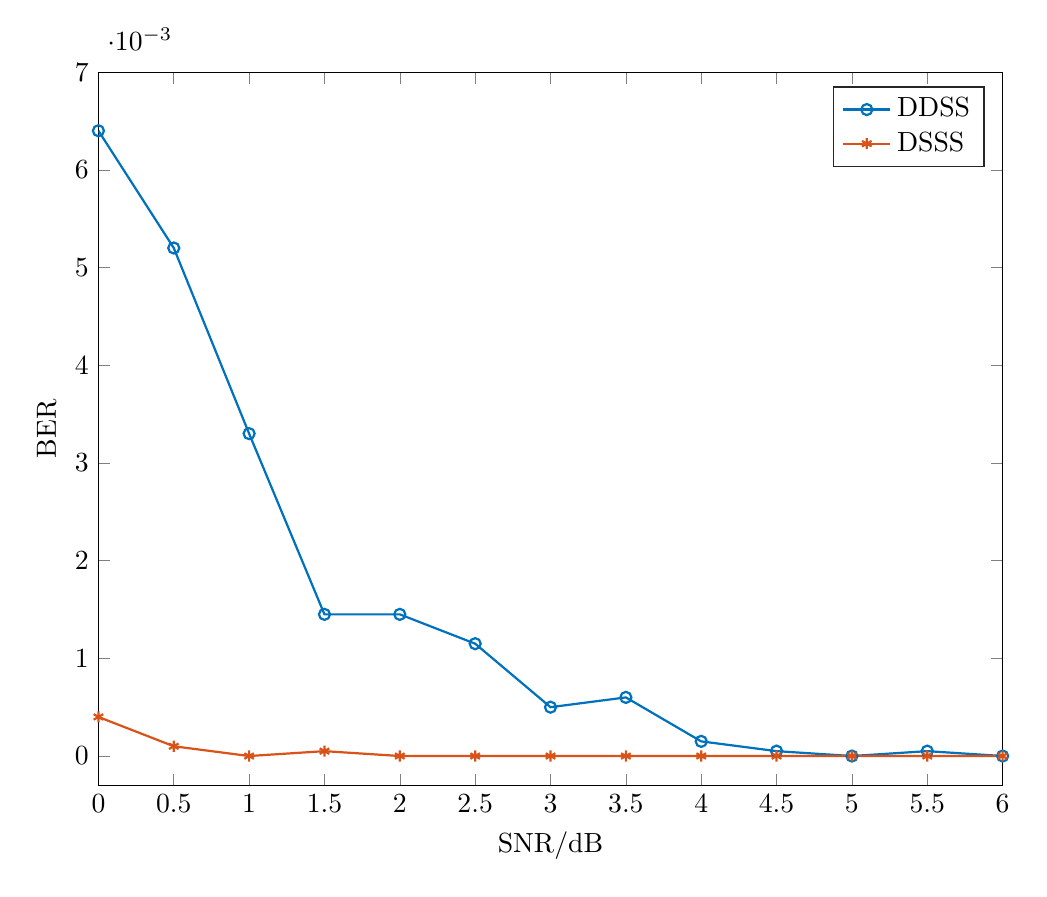
\begin{tikzpicture}

\begin{axis}[%
width=4.521in,
height=3.566in,
at={(0.758in,0.481in)},
scale only axis,
xmin=0,
xmax=6,
xlabel={SNR/dB},
ymin=-0.0003,
ymax=0.007,
ylabel={BER},
axis background/.style={fill=white},
legend style={legend cell align=left,align=left,draw=white!15!black}
]
\addplot [color=mycolor1,solid,line width=0.8pt,mark=o,mark options={solid}]
  table[row sep=crcr]{%
0	0.0064\\
0.5	0.0052\\
1	0.0033\\
1.5	0.00145\\
2	0.00145\\
2.5	0.00115\\
3	0.0005\\
3.5	0.0006\\
4	0.00015\\
4.5	5e-05\\
5	0\\
5.5	5e-05\\
6	0\\
};
\addlegendentry{DDSS};

\addplot [color=mycolor2,solid,line width=0.8pt,mark=asterisk,mark options={solid}]
  table[row sep=crcr]{%
0	0.0004\\
0.5	0.0001\\
1	0\\
1.5	5e-05\\
2	0\\
2.5	0\\
3	0\\
3.5	0\\
4	0\\
4.5	0\\
5	0\\
5.5	0\\
6	0\\
};
\addlegendentry{DSSS};

\end{axis}
\end{tikzpicture}%
	\caption{$\alpha=0$时DDSS和DSSS仿真误码率}
	\label{fig:software:dop0}
\end{figure}

图\ref{fig:software:sig}为$\alpha=10^{-4}$时接收信号经解调后的基带信号。根据\ref{sec:ddcode:dopuler}节分析,多普勒将会给基带信号引入一个频率为$\alpha f_c=0.3Hz$的拍频。根据式(\ref{equ:ddcode:td}),拍包络时间宽度为$T_D=\frac{1}{2\times0.3}=1.67s$。
根据式(\ref{equ:ddcode:sig}),由于载波不同步,基带信号的实部(虚部)将同时有原基带信号的实部与虚部。图中可见,有两个相互交错的起伏包络既是原实部与虚部叠加后导致的。
\begin{figure}[htbp]
	\centering
	% This file was created by matlab2tikz.
%
%The latest updates can be retrieved from
%  http://www.mathworks.com/matlabcentral/fileexchange/22022-matlab2tikz-matlab2tikz
%where you can also make suggestions and rate matlab2tikz.
%
\definecolor{mycolor1}{rgb}{0.00000,0.44700,0.74100}%
%
\begin{tikzpicture}

\begin{axis}[%
width=4.521in,
height=1.493in,
at={(0.758in,2.554in)},
scale only axis,
xmin=0,
xmax=7,
ymin=-4,
ymax=4,
xlabel={t/s},
ylabel={实部},
axis background/.style={fill=white}
]
\addplot [color=mycolor1,solid,forget plot]
  table[row sep=crcr]{%
0	-0.0219813001532536\\
0.002	-2.83832445303623\\
0.004	-2.80542310840654\\
0.006	2.86460017074594\\
0.008	-2.6002442200076\\
0.01	-2.74429854459139\\
0.012	2.50162321052841\\
0.014	-2.90676175339325\\
0.016	2.46408703898522\\
0.018	-2.6651770378808\\
0.02	2.51675091339198\\
0.022	-2.6458749056906\\
0.024	2.67800739051919\\
0.026	-2.29232651097421\\
0.028	2.72547647844208\\
0.03	2.74774432435686\\
0.032	0.41464065077151\\
0.034	0.332707603731718\\
0.036	-0.466336294017676\\
0.038	0.407993540699147\\
0.04	0.453846614332209\\
0.042	-0.495202796466844\\
0.044	0.489949990862283\\
0.046	-0.354599679327149\\
0.048	0.579480622410776\\
0.05	-0.530655531481323\\
0.052	0.457121268267698\\
0.054	-0.446785751197687\\
0.056	0.333309096916355\\
0.058	-0.319260999932288\\
0.06	-0.484481095132383\\
0.062	2.49072039212453\\
0.064	2.67883969393919\\
0.066	-2.73260565172497\\
0.068	2.49177092377981\\
0.07	2.59710584402407\\
0.072	-2.51527846578802\\
0.074	2.72856820714845\\
0.076	-2.5564946447362\\
0.078	2.69574619821139\\
0.08	-2.58300991820524\\
0.082	2.73682510348551\\
0.084	-2.58148879742014\\
0.086	2.33209504603688\\
0.088	-2.78048199288378\\
0.09	-2.49732296608517\\
0.092	-2.56112021091266\\
0.094	-2.49604753678452\\
0.096	2.51687976737454\\
0.098	-2.5121998869029\\
0.1	-2.61323330365899\\
0.102	2.5697672611857\\
0.104	-2.6834888170613\\
0.106	2.47887251928825\\
0.108	-2.44379481260296\\
0.11	2.30441300534606\\
0.112	-2.2444589024599\\
0.114	2.66480538686534\\
0.116	-2.57866273399851\\
0.118	2.54811436297921\\
0.12	2.62943896958181\\
0.122	-2.55455267411256\\
0.124	-2.52158038445058\\
0.126	2.70213596687662\\
0.128	-2.53392155180406\\
0.13	-2.48686836669176\\
0.132	2.588886434042\\
0.134	-2.44927610265937\\
0.136	2.4803893494336\\
0.138	-2.21935721051235\\
0.14	2.3372008311962\\
0.142	-2.64093083249702\\
0.144	2.38777128662909\\
0.146	-2.49637840414511\\
0.148	2.54117011984179\\
0.15	2.33667453687434\\
0.152	-2.61456021962432\\
0.154	-2.23582238957258\\
0.156	2.3780983582905\\
0.158	-2.61786622751335\\
0.16	-2.36075506228734\\
0.162	2.31902453568087\\
0.164	-2.2986733471702\\
0.166	2.35191000427291\\
0.168	-2.42217813478533\\
0.17	2.4760576807366\\
0.172	-2.2220732947148\\
0.174	2.49016838582201\\
0.176	-2.35512843969407\\
0.178	2.41139264986112\\
0.18	2.37379889325031\\
0.182	-1.16167125796252\\
0.184	-1.10953313780776\\
0.186	1.10861855251237\\
0.188	-1.33724212463975\\
0.19	-1.23418906742513\\
0.192	1.18923452597496\\
0.194	-1.31395423923943\\
0.196	1.33586937390789\\
0.198	-1.22207534847053\\
0.2	1.12313968238904\\
0.202	-1.05959603412017\\
0.204	1.18685253033581\\
0.206	-1.26322062153021\\
0.208	1.34448887876707\\
0.21	1.17968890805646\\
0.212	-1.08308276879736\\
0.214	-1.30474615737886\\
0.216	1.51040345055133\\
0.218	-1.42373859960101\\
0.22	-1.42151376371333\\
0.222	1.2429748469686\\
0.224	-1.1775154263857\\
0.226	1.20283857703507\\
0.228	-1.38185743355222\\
0.23	1.54188288101013\\
0.232	-1.26352696319687\\
0.234	1.23047431396021\\
0.236	-1.39226704520934\\
0.238	1.40066854031146\\
0.24	1.26543789828084\\
0.242	1.35431723133224\\
0.244	1.30080288600705\\
0.246	-1.22169505692518\\
0.248	1.47716912329062\\
0.25	1.40391356721084\\
0.252	-1.36965237291033\\
0.254	1.68203942805504\\
0.256	-1.73146811175566\\
0.258	1.43893979726766\\
0.26	-1.34790052869171\\
0.262	1.28968545437372\\
0.264	-1.26594073283255\\
0.266	1.33951396514048\\
0.268	-1.53837664672007\\
0.27	-1.49447742336553\\
0.272	-2.18217430039942\\
0.274	-2.24818793493758\\
0.276	2.1515961697486\\
0.278	-2.28718356781732\\
0.28	-2.06921081780972\\
0.282	2.38962572737951\\
0.284	-2.19149160940681\\
0.286	2.23001965996483\\
0.288	-2.07795346098093\\
0.29	2.21336048464285\\
0.292	-2.00154013261971\\
0.294	2.39378674816611\\
0.296	-2.38470080710747\\
0.298	2.38020341971658\\
0.3	2.47724066720573\\
0.302	-2.03886622506546\\
0.304	-2.15374928492075\\
0.306	2.33431252959017\\
0.308	-1.90342398117904\\
0.31	-2.30353015873698\\
0.312	2.00189948449148\\
0.314	-1.92379922386949\\
0.316	1.95562976906844\\
0.318	-1.86417475001669\\
0.32	1.74870531609121\\
0.322	-1.67678822181623\\
0.324	2.19153919938478\\
0.326	-1.97058495584169\\
0.328	1.96401007353401\\
0.33	2.16563910112239\\
0.332	-1.76371110004523\\
0.334	-1.59299765809336\\
0.336	1.62950982683466\\
0.338	-1.79075089125988\\
0.34	-1.65531141608932\\
0.342	1.81627139124657\\
0.344	-1.68576705341617\\
0.346	1.41625426343403\\
0.348	-2.02784837340471\\
0.35	1.7026416453175\\
0.352	-1.8586430571004\\
0.354	1.72297375347762\\
0.356	-1.55662805425282\\
0.358	1.88976205789731\\
0.36	1.82134567561926\\
0.362	-1.89987205704345\\
0.364	-1.98561601008987\\
0.366	2.0174336101906\\
0.368	-1.94773927288878\\
0.37	-1.58634608521906\\
0.372	1.82355704110639\\
0.374	-1.81881249303409\\
0.376	1.75963851972238\\
0.378	-1.81055217707663\\
0.38	1.98732259898394\\
0.382	-1.80226116445482\\
0.384	1.78906724658063\\
0.386	-1.63439164217023\\
0.388	1.65143242222868\\
0.39	1.97777178317327\\
0.392	1.86491158316883\\
0.394	1.70069739976684\\
0.396	-1.98482306821785\\
0.398	1.73054884976282\\
0.4	1.93275134192251\\
0.402	-1.67579466680705\\
0.404	1.69305074152728\\
0.406	-1.71809837004399\\
0.408	1.41425858017807\\
0.41	-1.80840156755817\\
0.412	1.60465767837946\\
0.414	-1.32051996167387\\
0.416	1.83367543811253\\
0.418	-1.77956813639441\\
0.42	-1.67622790092957\\
0.422	1.58022601110627\\
0.424	1.80638368476107\\
0.426	-1.50756526764835\\
0.428	1.7147778753404\\
0.43	1.59603041060854\\
0.432	-1.44930414067041\\
0.434	1.5636194855058\\
0.436	-1.73690180307275\\
0.438	1.55938566721364\\
0.44	-1.77392176876892\\
0.442	1.56995190927372\\
0.444	-1.80011674863745\\
0.446	1.69712426422545\\
0.448	-1.54946710988503\\
0.45	-1.63197682391978\\
0.452	2.20811596405027\\
0.454	2.21465768443571\\
0.456	-2.14468955422952\\
0.458	2.03061477197846\\
0.46	2.20511894603309\\
0.462	-2.03283989209627\\
0.464	2.21487027705272\\
0.466	-2.09899473004285\\
0.468	2.21755015403296\\
0.47	-1.88732572987343\\
0.472	2.12695175790297\\
0.474	-2.260740862465\\
0.476	2.37093916836327\\
0.478	-1.84165179504518\\
0.48	-2.40752266046777\\
0.482	1.43615234881975\\
0.484	1.57352772343106\\
0.486	-1.23620346062166\\
0.488	1.09881084202675\\
0.49	1.59258407339952\\
0.492	-1.56201477217811\\
0.494	1.14787470858356\\
0.496	-1.26240291589595\\
0.498	1.26949571105122\\
0.5	-1.56497641160533\\
0.502	1.45672185584926\\
0.504	-1.50962968815651\\
0.506	1.39697670698214\\
0.508	-1.30687641339714\\
0.51	-1.3125987826609\\
0.512	2.31340513375008\\
0.514	2.21866504362224\\
0.516	-1.96511897640148\\
0.518	2.11996683473591\\
0.52	2.1889227666339\\
0.522	-2.21823688911648\\
0.524	2.17721647871029\\
0.526	-2.39967221615635\\
0.528	2.37799931079844\\
0.53	-2.22293968822195\\
0.532	2.21548676002518\\
0.534	-2.52961672099353\\
0.536	2.26451611191119\\
0.538	-2.40431992698586\\
0.54	-2.25600037396567\\
0.542	2.21091464991968\\
0.544	2.27622388146113\\
0.546	-2.32916350375711\\
0.548	2.32173268460306\\
0.55	2.50038994200937\\
0.552	-2.2255868065951\\
0.554	2.30502869049498\\
0.556	-2.32557826423798\\
0.558	2.37539342621097\\
0.56	-2.39870133604593\\
0.562	2.47725746880207\\
0.564	-2.28289180705492\\
0.566	2.44427127686245\\
0.568	-2.40699953116173\\
0.57	-2.43177520356466\\
0.572	-2.50092012438041\\
0.574	-2.44104473361255\\
0.576	2.54946306553402\\
0.578	-2.44173175148957\\
0.58	-2.36224060183476\\
0.582	2.50570279440309\\
0.584	-2.13141894600069\\
0.586	2.51063441251277\\
0.588	-2.46103304308265\\
0.59	2.33335781889712\\
0.592	-2.4245804241784\\
0.594	2.18277446255623\\
0.596	-2.63947693303206\\
0.598	2.22697206878185\\
0.6	2.64202734874037\\
0.602	-2.39295199396487\\
0.604	-2.50861055277041\\
0.606	2.57541689692291\\
0.608	-2.50920322110442\\
0.61	-2.51067292755936\\
0.612	2.6471089852827\\
0.614	-2.42492579665901\\
0.616	2.40721527693974\\
0.618	-2.36788970545196\\
0.62	2.40962129316117\\
0.622	-2.72615481520834\\
0.624	2.40230686475911\\
0.626	-2.42581851861865\\
0.628	2.5585849919326\\
0.63	2.58708527536944\\
0.632	2.23369606810608\\
0.634	2.58790500844974\\
0.636	-2.59430496363779\\
0.638	2.62789487986115\\
0.64	2.55667102101154\\
0.642	-2.39966705521613\\
0.644	2.6412363628106\\
0.646	-2.47235390675272\\
0.648	2.24339100099362\\
0.65	-2.67796478978131\\
0.652	2.507684023061\\
0.654	-2.67983120885157\\
0.656	2.73843764693661\\
0.658	-2.2705407796112\\
0.66	-2.60385069591043\\
0.662	-0.477687177736828\\
0.664	-0.634914271430648\\
0.666	0.531520863177233\\
0.668	-0.733581976114624\\
0.67	-0.706630887876416\\
0.672	0.67586065716722\\
0.674	-0.711046537433154\\
0.676	0.366686974813685\\
0.678	-0.558078083085469\\
0.68	0.444152356465531\\
0.682	-0.426584659523251\\
0.684	0.670683793726417\\
0.686	-0.802403150118416\\
0.688	0.642123042306262\\
0.69	0.550764433538229\\
0.692	-0.379287841170469\\
0.694	-0.516749116499946\\
0.696	0.382969700410129\\
0.698	-0.368594838974542\\
0.7	-0.392961502849923\\
0.702	0.431151433771332\\
0.704	-0.533303430866491\\
0.706	0.18246461226867\\
0.708	-0.195708201004816\\
0.71	0.208775327389917\\
0.712	-0.605755164645815\\
0.714	0.123713802928338\\
0.716	-0.618191458086919\\
0.718	0.398701152563224\\
0.72	0.573354638493556\\
0.722	-0.379011845848097\\
0.724	-0.280575717164394\\
0.726	0.576916811816382\\
0.728	-0.245791689463422\\
0.73	-0.534014930003399\\
0.732	0.420607399677469\\
0.734	-0.120258972292014\\
0.736	0.538216166798321\\
0.738	-0.0551504601899793\\
0.74	0.394522749194371\\
0.742	-0.00414574773885727\\
0.744	0.161803989952682\\
0.746	-0.292527745115942\\
0.748	0.0230647979190094\\
0.75	0.194130006356318\\
0.752	-0.119273937958902\\
0.754	-0.262411299569144\\
0.756	0.287514006507907\\
0.758	-0.0962512248968394\\
0.76	-0.308257192133034\\
0.762	0.125838713210504\\
0.764	-0.00538636119026131\\
0.766	0.167078683353381\\
0.768	-0.315459281853574\\
0.77	0.0870224892153685\\
0.772	-0.28432132745161\\
0.774	-0.0182592390919366\\
0.776	0.10131500800799\\
0.778	0.0974048810070704\\
0.78	-0.0261486409546587\\
0.782	-2.47208331998833\\
0.784	-2.76858693160401\\
0.786	2.73467921622548\\
0.788	-2.62767304959123\\
0.79	-2.80455953910616\\
0.792	2.54206032700751\\
0.794	-2.61946397196375\\
0.796	2.45039025967075\\
0.798	-2.88341472575722\\
0.8	2.49782782903936\\
0.802	-2.58735197737639\\
0.804	2.50557920272053\\
0.806	-2.70827263360175\\
0.808	2.45943519457997\\
0.81	2.51314578690884\\
0.812	0.526908318746219\\
0.814	0.146700549437917\\
0.816	-0.242850579848981\\
0.818	-0.197648903696473\\
0.82	0.234624306496377\\
0.822	-0.134058542093845\\
0.824	0.133550849329116\\
0.826	-0.230000044463928\\
0.828	0.224155051875335\\
0.83	-0.155112304850069\\
0.832	0.195669911978788\\
0.834	-0.0955336388740382\\
0.836	0.326650688115322\\
0.838	-0.042629365186878\\
0.84	-0.477988512817039\\
0.842	-2.54370627951608\\
0.844	-2.6546340517369\\
0.846	2.67665671659247\\
0.848	-2.6778901243113\\
0.85	-2.88737733812959\\
0.852	2.59156914733849\\
0.854	-2.6631970175313\\
0.856	2.8181902718185\\
0.858	-2.7489066804708\\
0.86	2.70376034512724\\
0.862	-2.56769713974152\\
0.864	2.44853163035257\\
0.866	-2.46431833994061\\
0.868	2.54941220476132\\
0.87	2.46643811765971\\
0.872	0.449181945036443\\
0.874	0.108059178205651\\
0.876	-0.262285691626395\\
0.878	0.264607748674758\\
0.88	0.477291649984423\\
0.882	-0.711681628749038\\
0.884	0.504235007138892\\
0.886	-0.202811715626435\\
0.888	0.366279136461977\\
0.89	-0.314768306238923\\
0.892	0.534157121503456\\
0.894	-0.512399743134657\\
0.896	0.532245207380617\\
0.898	-0.429948305662233\\
0.9	-0.390392184179883\\
0.902	0.466508782746855\\
0.904	0.649776862338408\\
0.906	-0.654579499444809\\
0.908	0.618125272056931\\
0.91	0.621325378261149\\
0.912	-0.468280909238195\\
0.914	0.519438044667539\\
0.916	-0.750871557747769\\
0.918	0.520315365642934\\
0.92	-0.601119732992932\\
0.922	0.618972863704964\\
0.924	-0.508865204792797\\
0.926	0.692435492701296\\
0.928	-0.976257798873426\\
0.93	-0.481621863821831\\
0.932	-2.5678850242945\\
0.934	-2.71287498289376\\
0.936	2.62755624277491\\
0.938	-2.56998661796352\\
0.94	-2.55208305820188\\
0.942	2.43818200172608\\
0.944	-2.70300719071015\\
0.946	2.41346832319908\\
0.948	-2.52062680938496\\
0.95	2.43242814539541\\
0.952	-2.5296100191751\\
0.954	2.41524206015715\\
0.956	-2.77849249710149\\
0.958	2.28622551937269\\
0.96	2.5490771318547\\
0.962	0.865348804870814\\
0.964	0.977840254085299\\
0.966	-0.98284701823279\\
0.968	0.867799968695287\\
0.97	0.649011647123192\\
0.972	-1.1638500764817\\
0.974	0.566686969604355\\
0.976	-0.947735205088094\\
0.978	0.78795005157755\\
0.98	-0.955018452518451\\
0.982	1.15538996339934\\
0.984	-1.09917365617993\\
0.986	0.813629866410118\\
0.988	-0.948592645238322\\
0.99	-1.23874571304489\\
0.992	1.12954445539023\\
0.994	0.884902057135321\\
0.996	-1.06331089061158\\
0.998	1.00211722175228\\
1	1.00213856728106\\
1.002	-1.18315906703688\\
1.004	0.947028397528434\\
1.006	-0.99178206388652\\
1.008	1.1420686825082\\
1.01	-1.0610834872989\\
1.012	0.979801234704684\\
1.014	-1.1541440548379\\
1.016	0.737971148999277\\
1.018	-1.20834591417907\\
1.02	-1.343153473714\\
1.022	-1.27813525010003\\
1.024	-1.23089705045795\\
1.026	1.09979727002669\\
1.028	-1.27871185845435\\
1.03	-1.40964880838108\\
1.032	1.13272790662496\\
1.034	-1.29206665187562\\
1.036	1.05065962807499\\
1.038	-1.12192618138267\\
1.04	1.08992121465883\\
1.042	-1.45118866723364\\
1.044	1.19664473491654\\
1.046	-1.17734779549828\\
1.048	1.12160520372578\\
1.05	1.12240793381988\\
1.052	2.20197586120878\\
1.054	2.33935467427514\\
1.056	-2.18025467000683\\
1.058	2.35883620854367\\
1.06	2.4649186062871\\
1.062	-2.03192327840246\\
1.064	2.46620549706057\\
1.066	-2.18486530595376\\
1.068	2.3026642531944\\
1.07	-2.18998140489066\\
1.072	2.36851250633707\\
1.074	-2.12591394023056\\
1.076	2.06853460919319\\
1.078	-2.22496895477767\\
1.08	-2.25920150009715\\
1.082	2.32121801995916\\
1.084	2.14425460277046\\
1.086	-2.08109845095358\\
1.088	2.32495552211902\\
1.09	2.40089453062876\\
1.092	-2.09847666725934\\
1.094	2.23322481414191\\
1.096	-2.12724323967582\\
1.098	2.04792289293106\\
1.1	-2.14679936748787\\
1.102	2.39732722277497\\
1.104	-2.18087872281583\\
1.106	2.06745859014376\\
1.108	-2.25417013553789\\
1.11	-2.3151359495752\\
1.112	-1.45773503846872\\
1.114	-1.59978904469075\\
1.116	1.39731047810772\\
1.118	-1.55545475362096\\
1.12	-1.7693033744267\\
1.122	1.55879971342666\\
1.124	-1.45099137771127\\
1.126	1.47444873287398\\
1.128	-1.47487084776378\\
1.13	1.61292714885588\\
1.132	-1.33102016235929\\
1.134	1.72866457689384\\
1.136	-1.72091312241075\\
1.138	1.44478973280759\\
1.14	1.60547151904263\\
1.142	1.57952492805097\\
1.144	1.53325798744646\\
1.146	-1.42637519522071\\
1.148	1.48289589084724\\
1.15	1.73486317774784\\
1.152	-1.37846805542267\\
1.154	1.52542335951107\\
1.156	-1.48360573049573\\
1.158	1.79479861333789\\
1.16	-1.82315685882233\\
1.162	1.70925054437311\\
1.164	-1.40477974165566\\
1.166	1.51418203069083\\
1.168	-1.57699128703734\\
1.17	-1.77300873163213\\
1.172	-1.71935811932712\\
1.174	-1.77252074189099\\
1.176	1.88035485193138\\
1.178	-1.80929848702471\\
1.18	-1.83144324464377\\
1.182	1.74915026350591\\
1.184	-1.65406914547004\\
1.186	1.86933353757336\\
1.188	-1.85985165308811\\
1.19	1.8010591954396\\
1.192	-1.93004367087134\\
1.194	1.91859534588528\\
1.196	-1.74751153884955\\
1.198	1.79473331947503\\
1.2	1.94676964117305\\
1.202	-1.95193192407336\\
1.204	-1.86258360834399\\
1.206	1.81148724610291\\
1.208	-1.89214740862414\\
1.21	-1.71698830619102\\
1.212	1.94277744286718\\
1.214	-1.76607882342015\\
1.216	1.88669116527588\\
1.218	-1.81528710934098\\
1.22	1.89037242246235\\
1.222	-2.05264253508044\\
1.224	2.35880112040343\\
1.226	-1.90997867635591\\
1.228	2.1014756770577\\
1.23	2.06656022603857\\
1.232	-2.05294648642643\\
1.234	-2.21602007627671\\
1.236	1.76401888846755\\
1.238	-2.27780306942599\\
1.24	-1.9323847533267\\
1.242	2.05173298378694\\
1.244	-2.13816019266763\\
1.246	1.87063311397152\\
1.248	-2.08814416871163\\
1.25	1.85589436152079\\
1.252	-1.89087391007852\\
1.254	2.00897684685672\\
1.256	-2.03493338414855\\
1.258	2.09447425187615\\
1.26	2.05824966165168\\
1.262	1.46587436829719\\
1.264	1.68043955194827\\
1.266	-1.74661879828099\\
1.268	1.67985888287955\\
1.27	1.87092967564499\\
1.272	-1.72203074378779\\
1.274	1.33655901274224\\
1.276	-1.80608023590946\\
1.278	1.59647836196401\\
1.28	-1.59944325155624\\
1.282	1.39345206393871\\
1.284	-1.59448444763332\\
1.286	1.6620972466256\\
1.288	-1.76869834318455\\
1.29	-1.63364167535216\\
1.292	1.55684464011275\\
1.294	1.39710331469257\\
1.296	-1.34588616239909\\
1.298	1.69272953142782\\
1.3	1.64870354565648\\
1.302	-1.39270162298814\\
1.304	1.35737176851398\\
1.306	-1.2538593006377\\
1.308	1.22877837935607\\
1.31	-1.35369288178467\\
1.312	1.28519436856876\\
1.314	-1.42253627560587\\
1.316	1.44148205703795\\
1.318	-1.59919955182524\\
1.32	-1.51244007289652\\
1.322	2.21808153443936\\
1.324	2.14024298962024\\
1.326	-2.00397835294971\\
1.328	2.00998763091618\\
1.33	2.26939461366975\\
1.332	-2.31211590218216\\
1.334	2.35752955064938\\
1.336	-2.08963042391295\\
1.338	2.36023590879246\\
1.34	-2.23327027372485\\
1.342	2.14121752702898\\
1.344	-2.13523481184618\\
1.346	2.26647195251688\\
1.348	-2.38921566455403\\
1.35	-2.40418075863255\\
1.352	2.17367965274138\\
1.354	2.40456981601113\\
1.356	-2.08187923848981\\
1.358	2.43469877419521\\
1.36	2.14691061278056\\
1.362	-2.36920063387299\\
1.364	2.40259840456042\\
1.366	-2.16981721581848\\
1.368	2.55275403883944\\
1.37	-2.38581664825468\\
1.372	2.36036601677016\\
1.374	-2.30860904576954\\
1.376	2.32034876321917\\
1.378	-2.30216979981682\\
1.38	-2.50085662097746\\
1.382	-2.46628329634341\\
1.384	-2.6801292041256\\
1.386	2.36547096072426\\
1.388	-2.27700965401319\\
1.39	-2.56722406825376\\
1.392	2.3752946000138\\
1.394	-2.15483313822992\\
1.396	2.5601953704646\\
1.398	-2.45405200272799\\
1.4	2.45964834241961\\
1.402	-2.35412002153458\\
1.404	2.35443814350957\\
1.406	-2.29791027007602\\
1.408	2.26463724547797\\
1.41	2.31812138006415\\
1.412	-0.961664390716227\\
1.414	-1.03298055747092\\
1.416	1.17422774643888\\
1.418	-0.890389812624976\\
1.42	-1.01978772417981\\
1.422	0.947253780267589\\
1.424	-0.798542990732322\\
1.426	0.67717422743786\\
1.428	-0.876318142262997\\
1.43	0.836394766852006\\
1.432	-1.05451378783106\\
1.434	1.02383191021253\\
1.436	-1.0749002946804\\
1.438	0.945942822814066\\
1.44	0.921102026053216\\
1.442	1.15232684970395\\
1.444	0.926736265838493\\
1.446	-0.877592924140612\\
1.448	0.580072977056855\\
1.45	0.732397413986146\\
1.452	-0.850175809797657\\
1.454	1.15587852593673\\
1.456	-0.638103507656518\\
1.458	0.802705624966233\\
1.46	-0.823487254100898\\
1.462	0.558726400453615\\
1.464	-0.786737771021966\\
1.466	0.907969150558154\\
1.468	-0.882349506155118\\
1.47	-0.836335382947453\\
1.472	-0.636644760912761\\
1.474	-0.604451803591034\\
1.476	0.823649833543747\\
1.478	-0.909342268971015\\
1.48	-0.90517981153315\\
1.482	0.617010645310175\\
1.484	-0.633621234997925\\
1.486	0.549416381329322\\
1.488	-0.738811412836515\\
1.49	0.844933808896046\\
1.492	-0.458713242673095\\
1.494	0.704351762623009\\
1.496	-0.728409866190045\\
1.498	0.820538535964851\\
1.5	0.782690527845614\\
1.502	-2.64075328831992\\
1.504	-2.64961104586773\\
1.506	2.5432795560888\\
1.508	-2.68259527924058\\
1.51	-2.54946358087443\\
1.512	2.38964721747918\\
1.514	-2.57031639201233\\
1.516	2.53143947954059\\
1.518	-2.87209007328431\\
1.52	2.58280590009177\\
1.522	-2.59569445505445\\
1.524	2.61929680023374\\
1.526	-2.44578266180319\\
1.528	2.42581210176502\\
1.53	2.54491014608078\\
1.532	-0.165189939019551\\
1.534	-0.478154459832379\\
1.536	0.650737868111412\\
1.538	-0.351242108011244\\
1.54	-0.0285469083207002\\
1.542	0.255441034522381\\
1.544	-0.500085181752589\\
1.546	0.498744054881901\\
1.548	-0.594677007047808\\
1.55	0.205270446641327\\
1.552	-0.114871124968701\\
1.554	0.552893540268487\\
1.556	-0.298635447373531\\
1.558	0.391577681739464\\
1.56	0.0628006261350327\\
1.562	2.44434759964263\\
1.564	2.45087356634484\\
1.566	-2.62881776281433\\
1.568	2.67426890611706\\
1.57	2.63820788865103\\
1.572	-2.33902087083276\\
1.574	2.65636651497559\\
1.576	-2.41173183553278\\
1.578	2.64683702533983\\
1.58	-2.49393814772149\\
1.582	2.48175555607597\\
1.584	-2.30053767758023\\
1.586	2.5440741140388\\
1.588	-2.60643241271799\\
1.59	-2.6201763334953\\
1.592	-0.197068096398242\\
1.594	0.219994692811984\\
1.596	-0.0581353160474999\\
1.598	0.296377924872098\\
1.6	0.238350873077958\\
1.602	-0.0345262066631127\\
1.604	-0.0913346328317631\\
1.606	0.0202480303870358\\
1.608	0.25406293980077\\
1.61	-0.235480541598742\\
1.612	0.0840800329644136\\
1.614	-0.392135963112743\\
1.616	0.132338611168908\\
1.618	-0.0373510285728755\\
1.62	-0.0191722575585452\\
1.622	2.68194507443981\\
1.624	2.60540880308302\\
1.626	-2.37247798410036\\
1.628	2.44773606767071\\
1.63	2.47896056410689\\
1.632	-2.41591438086487\\
1.634	2.56986139114519\\
1.636	-2.51174244251768\\
1.638	2.60470237008995\\
1.64	-2.54398814898484\\
1.642	2.26809399513889\\
1.644	-2.70609556239599\\
1.646	2.70201310660121\\
1.648	-2.20760844706992\\
1.65	-2.6097388701495\\
1.652	0.0120388341062446\\
1.654	0.105361653701888\\
1.656	-0.355515889237467\\
1.658	0.367682365584781\\
1.66	0.247387067906806\\
1.662	-0.361654382378603\\
1.664	0.0496236210342797\\
1.666	0.0108865192686472\\
1.668	0.088540926085733\\
1.67	-0.249548719563281\\
1.672	0.103822415279704\\
1.674	-0.267182507019036\\
1.676	0.322477636050899\\
1.678	-0.324794680735877\\
1.68	-0.0853460527515125\\
1.682	-0.112785418726409\\
1.684	-0.381650155740342\\
1.686	0.273736490965\\
1.688	-0.308165457162188\\
1.69	-0.098954731467413\\
1.692	0.378535702652821\\
1.694	-0.262635465686436\\
1.696	-0.0260796066852346\\
1.698	-0.305787811886878\\
1.7	0.736945592983213\\
1.702	-0.437965717353267\\
1.704	0.410918161299673\\
1.706	-0.339824607538154\\
1.708	0.489486170516995\\
1.71	0.709540235151588\\
1.712	2.49627768186987\\
1.714	2.58985042983263\\
1.716	-2.52361381416143\\
1.718	2.44316829707698\\
1.72	2.77006884586352\\
1.722	-2.70189761485743\\
1.724	2.32222303489224\\
1.726	-2.61032809343503\\
1.728	2.39070903216303\\
1.73	-2.42342633418082\\
1.732	2.48709457917189\\
1.734	-2.40233693920842\\
1.736	2.62985071615307\\
1.738	-2.41873086330061\\
1.74	-2.64751191748471\\
1.742	2.71026634440543\\
1.744	2.79733667729532\\
1.746	-2.60111910056676\\
1.748	2.315624178974\\
1.75	2.54115276787153\\
1.752	-2.56259520969432\\
1.754	2.50638386481335\\
1.756	-2.38991194838567\\
1.758	2.67849459357315\\
1.76	-2.42978443953812\\
1.762	2.51450346242806\\
1.764	-2.36227857275548\\
1.766	2.4752676277876\\
1.768	-2.50088046392483\\
1.77	-2.66317072611388\\
1.772	0.592608029295841\\
1.774	0.7194757342444\\
1.776	-0.649459061318102\\
1.778	0.726274056284482\\
1.78	0.61082406239577\\
1.782	-0.796433318969388\\
1.784	1.07659093013028\\
1.786	-0.528949875330478\\
1.788	0.647935011317989\\
1.79	-0.787916709337522\\
1.792	0.774812562007787\\
1.794	-0.846156494159286\\
1.796	0.834248034396928\\
1.798	-0.754065642700449\\
1.8	-0.68893717338249\\
1.802	-2.9120351165837\\
1.804	-2.4345153934748\\
1.806	2.13273964139172\\
1.808	-2.42528836766489\\
1.81	-2.53390504113094\\
1.812	2.26920582447246\\
1.814	-2.49710795454859\\
1.816	2.36069596966773\\
1.818	-2.27463742851573\\
1.82	2.55012353370744\\
1.822	-2.26009202172104\\
1.824	2.44333357599492\\
1.826	-2.36203034906463\\
1.828	2.14780858856915\\
1.83	2.28581603427087\\
1.832	2.46488688748973\\
1.834	2.58470266798012\\
1.836	-2.26864400280071\\
1.838	2.44994402980751\\
1.84	2.44629862404451\\
1.842	-2.32534451972135\\
1.844	2.21357141611762\\
1.846	-2.11143283178625\\
1.848	2.08615919750656\\
1.85	-2.39945771303045\\
1.852	2.49310134055835\\
1.854	-2.35421059902983\\
1.856	2.30302758396831\\
1.858	-1.8982074842924\\
1.86	-2.50544045335431\\
1.862	-1.13760487087192\\
1.864	-1.09278477399606\\
1.866	1.3131745438534\\
1.868	-1.09847830275174\\
1.87	-1.32458450253761\\
1.872	0.885386958541065\\
1.874	-1.03839684627159\\
1.876	1.1478150634697\\
1.878	-1.07143502577448\\
1.88	1.06874460971772\\
1.882	-1.17569908618283\\
1.884	1.3168715281265\\
1.886	-0.94317877878856\\
1.888	1.23925579181184\\
1.89	1.25281824032706\\
1.892	1.31412121555936\\
1.894	1.2626647081715\\
1.896	-1.36145969248286\\
1.898	1.16633706678356\\
1.9	1.34113926650611\\
1.902	-1.20106249420591\\
1.904	1.30352597725386\\
1.906	-1.18601775059963\\
1.908	1.0681265438263\\
1.91	-1.3186352074789\\
1.912	1.0989741777647\\
1.914	-1.24145641345914\\
1.916	1.48265044369452\\
1.918	-1.19213957434383\\
1.92	-1.41604551361962\\
1.922	2.15591248561001\\
1.924	2.3431729555893\\
1.926	-1.93776538211141\\
1.928	2.26028829327423\\
1.93	2.35373816908833\\
1.932	-2.14088598233496\\
1.934	2.31301720576812\\
1.936	-2.07050040908823\\
1.938	2.1985380122959\\
1.94	-2.23509649954276\\
1.942	1.97120173326109\\
1.944	-2.07020431195423\\
1.946	2.03224651364322\\
1.948	-2.11308741318896\\
1.95	-2.06526053087973\\
1.952	1.88172993676321\\
1.954	2.22774440949664\\
1.956	-2.01210369918279\\
1.958	1.90269862599349\\
1.96	2.17565493853506\\
1.962	-1.88376665804392\\
1.964	2.06102025014372\\
1.966	-1.90299884143204\\
1.968	2.10670444945677\\
1.97	-2.12704549116366\\
1.972	1.54054567151611\\
1.974	-1.87555400046417\\
1.976	1.92671405082386\\
1.978	-1.95952489009414\\
1.98	-1.91170603906797\\
1.982	-1.76737855209481\\
1.984	-1.50339493748786\\
1.986	1.58239575195944\\
1.988	-1.31224749854137\\
1.99	-1.47997581346188\\
1.992	1.43679430128781\\
1.994	-1.42051243941092\\
1.996	1.5465691135076\\
1.998	-1.75240872835926\\
2	1.53093666987707\\
2.002	-1.62111773513954\\
2.004	1.78896060685965\\
2.006	-1.45985975230267\\
2.008	1.69545894948194\\
2.01	1.75465263157303\\
2.012	-1.86740870753456\\
2.014	-2.15829802795671\\
2.016	1.72311744821419\\
2.018	-1.88647866325926\\
2.02	-2.09705147994689\\
2.022	1.96339731562674\\
2.024	-1.55011485936415\\
2.026	2.01307977366273\\
2.028	-1.75505538915581\\
2.03	1.92397495014292\\
2.032	-1.74229392051436\\
2.034	1.7000476070551\\
2.036	-1.80911153152414\\
2.038	1.78664341664847\\
2.04	1.95550850985839\\
2.042	2.119039329263\\
2.044	1.94219060506115\\
2.046	-1.64513008908798\\
2.048	1.43664915459174\\
2.05	1.8086189809309\\
2.052	-1.6116735862853\\
2.054	1.64577527729443\\
2.056	-1.83294769360867\\
2.058	1.55868186129443\\
2.06	-1.84147994446589\\
2.062	1.79598219557284\\
2.064	-1.85036708233671\\
2.066	1.58370116248727\\
2.068	-1.55560662028127\\
2.07	-1.688048960393\\
2.072	-1.75939611193708\\
2.074	-1.60278986365572\\
2.076	1.62151584129703\\
2.078	-1.42945755806092\\
2.08	-1.66733360347709\\
2.082	1.51884104131071\\
2.084	-1.51249802037144\\
2.086	1.65200059880549\\
2.088	-1.49860328638705\\
2.09	1.435745043062\\
2.092	-1.59473035448684\\
2.094	1.54921349310013\\
2.096	-1.54283713755462\\
2.098	1.64402938389395\\
2.1	1.65991588066408\\
2.102	-2.17306307583345\\
2.104	-1.89587205131114\\
2.106	1.89570040181121\\
2.108	-1.92131851291919\\
2.11	-1.94083459617882\\
2.112	1.93029241129514\\
2.114	-1.76848872380023\\
2.116	1.70220264153488\\
2.118	-1.85426953497604\\
2.12	1.92297101630237\\
2.122	-1.85415867931795\\
2.124	1.94976649746468\\
2.126	-1.95395941315983\\
2.128	2.04446491164642\\
2.13	2.26890834720614\\
2.132	2.28469035253447\\
2.134	2.22930717615826\\
2.136	-1.99972137699175\\
2.138	2.08359973571476\\
2.14	2.42547947044591\\
2.142	-2.21429135015185\\
2.144	2.21625005271183\\
2.146	-2.08327145269588\\
2.148	1.83145651627731\\
2.15	-1.98632550178751\\
2.152	1.9011860093838\\
2.154	-2.09100878838442\\
2.156	1.98219647758414\\
2.158	-2.05402110194497\\
2.16	-2.39648388200615\\
2.162	1.2139005330952\\
2.164	1.38672510084756\\
2.166	-1.28467829759929\\
2.168	1.21111669250813\\
2.17	1.38843370563328\\
2.172	-1.38099517938837\\
2.174	1.27051786561487\\
2.176	-1.22698957462764\\
2.178	1.4241903067688\\
2.18	-1.08127596193344\\
2.182	1.29232134178169\\
2.184	-1.24528981153916\\
2.186	1.31359274005192\\
2.188	-1.2109359035998\\
2.19	-1.25535017524692\\
2.192	-2.42265740863445\\
2.194	-2.03147960503128\\
2.196	2.15665535160013\\
2.198	-2.09905057186674\\
2.2	-2.55016165950786\\
2.202	2.36150924368647\\
2.204	-2.23130986086476\\
2.206	1.94020543478566\\
2.208	-2.2913292933972\\
2.21	2.32749643852413\\
2.212	-2.30882912997261\\
2.214	2.03484140383904\\
2.216	-2.09109696745545\\
2.218	2.3971275470156\\
2.22	2.23765601730439\\
2.222	2.40443929024874\\
2.224	2.27369975940895\\
2.226	-1.95488277836733\\
2.228	2.16446466145981\\
2.23	2.32276838969944\\
2.232	-2.25036898920534\\
2.234	2.09465232405682\\
2.236	-1.88969896363325\\
2.238	2.30760951920136\\
2.24	-2.37450238269284\\
2.242	2.29803323708922\\
2.244	-1.97215975508927\\
2.246	2.44201956331051\\
2.248	-2.17725153166209\\
2.25	-2.42104147910216\\
2.252	0.866811581449706\\
2.254	0.903570639031094\\
2.256	-0.681256412090233\\
2.258	0.618197046407808\\
2.26	0.880500648362669\\
2.262	-0.843802548052115\\
2.264	1.04518632032711\\
2.266	-0.56769732239849\\
2.268	0.816168559460586\\
2.27	-0.652942520442467\\
2.272	0.643470387838732\\
2.274	-0.705537483453022\\
2.276	0.659118923505187\\
2.278	-0.790920644794401\\
2.28	-0.887421954741258\\
2.282	-2.36065990787727\\
2.284	-2.41098041157579\\
2.286	2.39522767723082\\
2.288	-2.08343936071367\\
2.29	-2.15532730622281\\
2.292	2.15258940408593\\
2.294	-2.16092626194081\\
2.296	2.44065966889888\\
2.298	-2.23074505107694\\
2.3	2.36946003330289\\
2.302	-2.29391218032067\\
2.304	2.31055280906217\\
2.306	-2.24980918124596\\
2.308	2.56440565081497\\
2.31	2.58792435626586\\
2.312	-2.30029037553011\\
2.314	-2.45521126056472\\
2.316	2.40672351537383\\
2.318	-2.21914442909241\\
2.32	-2.69129361215463\\
2.322	2.5325861058442\\
2.324	-2.22909831400018\\
2.326	2.35859241030426\\
2.328	-2.32218763608934\\
2.33	2.39769429127631\\
2.332	-2.34792848896893\\
2.334	2.16297106196123\\
2.336	-2.1683364449655\\
2.338	2.37969017998182\\
2.34	2.50680166793711\\
2.342	-0.540775988972663\\
2.344	-0.620157966154164\\
2.346	0.47419755854207\\
2.348	-0.389910104931862\\
2.35	-0.521894209641947\\
2.352	0.448935946600374\\
2.354	-0.344152385580137\\
2.356	0.298573750149489\\
2.358	-0.380884714175588\\
2.36	0.33316640204082\\
2.362	-0.56103096825433\\
2.364	0.522568514266162\\
2.366	-0.292560842828999\\
2.368	0.462115047237898\\
2.37	0.52174515471042\\
2.372	2.4983201128026\\
2.374	2.73294083106227\\
2.376	-2.34706343719616\\
2.378	2.38284632366799\\
2.38	2.94282044860322\\
2.382	-2.24379965988046\\
2.384	2.38687765721773\\
2.386	-2.58135803408713\\
2.388	2.56606652502483\\
2.39	-2.33178686158013\\
2.392	2.38593852487748\\
2.394	-2.29301707201508\\
2.396	2.3812858214949\\
2.398	-2.44217223764689\\
2.4	-2.46336895069038\\
2.402	-0.391434784796393\\
2.404	-0.548487441429628\\
2.406	0.0407241919403169\\
2.408	-0.125997910788137\\
2.41	-0.0756611865285431\\
2.412	-0.101575964443504\\
2.414	-0.287846802113521\\
2.416	0.260800739857196\\
2.418	-0.154862466591372\\
2.42	0.0355362014452119\\
2.422	-0.228975284348257\\
2.424	0.276173355598103\\
2.426	-0.0840795141715395\\
2.428	0.18784986933445\\
2.43	0.248456694373045\\
2.432	-0.107683636874701\\
2.434	-0.0251446607334247\\
2.436	0.0818341285076619\\
2.438	-0.0579703964458242\\
2.44	-0.154614948906241\\
2.442	-0.00132999655791428\\
2.444	0.015888272811263\\
2.446	0.118833910109046\\
2.448	0.0957937239204202\\
2.45	0.00624079566149963\\
2.452	0.258658867258634\\
2.454	-0.126282128532699\\
2.456	0.100067792016145\\
2.458	0.0401135096600361\\
2.46	0.0424281793413138\\
2.462	-0.12096794266597\\
2.464	-0.0352738732558238\\
2.466	-0.293853487628788\\
2.468	0.166043666051546\\
2.47	0.0244807774658516\\
2.472	-0.16148081566736\\
2.474	0.177167060683851\\
2.476	-0.103134787936082\\
2.478	0.195979943904424\\
2.48	-0.130456813328126\\
2.482	0.187037755061226\\
2.484	-0.27927323146939\\
2.486	0.202584740964612\\
2.488	-0.147688897419495\\
2.49	0.126670607529954\\
2.492	-0.278324515710357\\
2.494	-0.362732557796039\\
2.496	0.149098889269692\\
2.498	-0.0462710670711614\\
2.5	-0.31470896798544\\
2.502	0.135473076723352\\
2.504	-0.457729831083504\\
2.506	0.125849999847258\\
2.508	-0.203190525918661\\
2.51	0.496324476074607\\
2.512	-0.323385876376047\\
2.514	0.233905380292261\\
2.516	-0.27968408750553\\
2.518	0.251011157143938\\
2.52	0.339953234543195\\
2.522	0.507005735402453\\
2.524	0.509777909403587\\
2.526	-0.461026364376039\\
2.528	0.422548712474695\\
2.53	0.305019331527314\\
2.532	-0.34227135363292\\
2.534	0.338886822346743\\
2.536	-0.237007938107454\\
2.538	0.138263896301714\\
2.54	-0.420606372859325\\
2.542	0.332455388922036\\
2.544	-0.339957196501676\\
2.546	0.300812783283908\\
2.548	-0.230487847616074\\
2.55	-0.316362643348749\\
2.552	2.58496177719554\\
2.554	2.71367444561889\\
2.556	-2.22730436842287\\
2.558	2.18943135429109\\
2.56	2.73639933360261\\
2.562	-2.44091866345809\\
2.564	2.2918440148361\\
2.566	-2.24252645331144\\
2.568	2.36310529575568\\
2.57	-2.31192919633075\\
2.572	2.20705041165497\\
2.574	-2.19377002992376\\
2.576	2.24468822436111\\
2.578	-2.5128820851744\\
2.58	-2.68757367737435\\
2.582	-1.08174953342797\\
2.584	-0.741163888281967\\
2.586	0.722063191092928\\
2.588	-0.701027847031197\\
2.59	-0.584011874732518\\
2.592	0.727099163945182\\
2.594	-0.605528149430451\\
2.596	0.720170492879677\\
2.598	-0.679756474830161\\
2.6	0.597013088491254\\
2.602	-0.746422522808479\\
2.604	0.752588584436278\\
2.606	-0.511489921716618\\
2.608	0.503232221496809\\
2.61	0.780485810945871\\
2.612	-2.3266772197105\\
2.614	-2.65680161458672\\
2.616	2.08979258891105\\
2.618	-2.49409867049561\\
2.62	-2.57184222416433\\
2.622	2.22822557869621\\
2.624	-2.25947465263169\\
2.626	2.04689403505816\\
2.628	-2.28893828210991\\
2.63	2.13663831685352\\
2.632	-2.07986450048289\\
2.634	2.3836554999754\\
2.636	-1.92135314502632\\
2.638	2.3808719879917\\
2.64	2.68578672911333\\
2.642	-2.21705211061801\\
2.644	-2.51015343307159\\
2.646	2.16026641415161\\
2.648	-2.14267235988064\\
2.65	-2.22421351927097\\
2.652	2.13902396676111\\
2.654	-1.98668446014636\\
2.656	2.0216369388228\\
2.658	-2.41119522643671\\
2.66	2.17678028521714\\
2.662	-2.18307288400859\\
2.664	2.28058973132278\\
2.666	-2.09350419340829\\
2.668	2.04255784227976\\
2.67	2.43596203896435\\
2.672	2.3370044488267\\
2.674	2.33239289070272\\
2.676	-2.1865955655416\\
2.678	2.15941767404243\\
2.68	2.43540800753916\\
2.682	-1.99584882419664\\
2.684	2.26008658296543\\
2.686	-2.17073127648806\\
2.688	2.10487638331281\\
2.69	-1.89362424068686\\
2.692	1.784803373829\\
2.694	-1.93362613590244\\
2.696	2.0882546518519\\
2.698	-2.05555251828607\\
2.7	-2.34725356894379\\
2.702	-1.29646908353403\\
2.704	-1.27040522281082\\
2.706	1.09340686325339\\
2.708	-1.05115406312502\\
2.71	-0.88589865410201\\
2.712	0.970577135368206\\
2.714	-0.854121095112482\\
2.716	0.808779578910005\\
2.718	-1.32796309348837\\
2.72	1.08668920501393\\
2.722	-1.05908367035499\\
2.724	0.98928294857133\\
2.726	-1.20386903452712\\
2.728	1.24695364935506\\
2.73	1.25256631664016\\
2.732	1.33036095150851\\
2.734	1.2946837926345\\
2.736	-1.33413521155785\\
2.738	1.1020140225356\\
2.74	1.50765714138216\\
2.742	-1.08859171772526\\
2.744	1.25726181331447\\
2.746	-1.56942281103156\\
2.748	1.39217527059795\\
2.75	-1.30199994581826\\
2.752	1.22714485328578\\
2.754	-1.38617010940653\\
2.756	1.12233018781679\\
2.758	-1.03922580831095\\
2.76	-1.5809697918137\\
2.762	1.24933482230812\\
2.764	1.52396668439856\\
2.766	-1.49657827870435\\
2.768	1.32879416123513\\
2.77	1.49742527730918\\
2.772	-1.29088551678702\\
2.774	1.39332213327168\\
2.776	-1.25940537803362\\
2.778	1.21675376577255\\
2.78	-1.25653819939965\\
2.782	1.53477218161876\\
2.784	-1.25149942727192\\
2.786	1.41725859915486\\
2.788	-1.38138331409226\\
2.79	-1.50938958939673\\
2.792	1.99154052660658\\
2.794	2.03227857971727\\
2.796	-2.09559190340981\\
2.798	1.93955752102381\\
2.8	2.10933612107291\\
2.802	-1.99740485038098\\
2.804	1.8880566271066\\
2.806	-1.7373080472307\\
2.808	1.96138734111782\\
2.81	-1.68332744327013\\
2.812	1.79756417286996\\
2.814	-1.89574613914928\\
2.816	2.14645926990582\\
2.818	-1.62012818993689\\
2.82	-2.13715421697072\\
2.822	-1.9486413256367\\
2.824	-1.52682786359404\\
2.826	1.58449586997253\\
2.828	-1.43868080696076\\
2.83	-1.55722834292146\\
2.832	1.33519964845797\\
2.834	-1.47493174593472\\
2.836	1.61643119846817\\
2.838	-1.3789923683652\\
2.84	1.5787213739751\\
2.842	-1.46476284155344\\
2.844	1.56818448107071\\
2.846	-1.7478704051908\\
2.848	1.56573092498142\\
2.85	1.79277754482075\\
2.852	-1.77610347488696\\
2.854	-1.77397238355419\\
2.856	1.78901507120368\\
2.858	-1.51646172749839\\
2.86	-1.99219979625079\\
2.862	1.76469030683894\\
2.864	-1.84367264085281\\
2.866	1.64503435188808\\
2.868	-1.76147091021473\\
2.87	1.58130573128293\\
2.872	-1.62721042221106\\
2.874	1.70897572999741\\
2.876	-1.79522259754039\\
2.878	1.66518109281951\\
2.88	1.82740829916983\\
2.882	1.75287492900017\\
2.884	1.70534240130539\\
2.886	-1.58495395862423\\
2.888	1.54090917568279\\
2.89	1.97279833888225\\
2.892	-1.46817109186023\\
2.894	1.57140037308321\\
2.896	-1.57452164084243\\
2.898	1.77717258672273\\
2.9	-1.49875123721696\\
2.902	1.63111236989172\\
2.904	-1.59310466476004\\
2.906	1.617200465798\\
2.908	-1.49441151040447\\
2.91	-1.63219746467752\\
2.912	1.43991680890993\\
2.914	1.9097094367625\\
2.916	-1.62984557063794\\
2.918	1.65312117452714\\
2.92	1.54582050551652\\
2.922	-1.45502226452209\\
2.924	1.3841358208672\\
2.926	-1.66351112900484\\
2.928	1.547880438321\\
2.93	-1.33473446522433\\
2.932	1.64904280964755\\
2.934	-1.5026831198952\\
2.936	1.34605130659159\\
2.938	-1.24417149570582\\
2.94	-1.73994806145834\\
2.942	-1.61444948535044\\
2.944	-1.51205275366386\\
2.946	1.28665311947534\\
2.948	-1.52509970682828\\
2.95	-1.50211506014745\\
2.952	1.55676458551974\\
2.954	-1.18268998869936\\
2.956	1.44662533977779\\
2.958	-1.4161534615476\\
2.96	1.13674799650446\\
2.962	-1.25769745536238\\
2.964	1.35254789570999\\
2.966	-1.47533042150248\\
2.968	1.17409651930749\\
2.97	1.64227280435255\\
2.972	2.18630391992533\\
2.974	2.13506668841487\\
2.976	-1.71065675343108\\
2.978	1.82484389874609\\
2.98	2.30587228419748\\
2.982	-1.95806246369374\\
2.984	1.98553552126533\\
2.986	-1.96379111823827\\
2.988	1.87839158291581\\
2.99	-1.89720024495374\\
2.992	1.90873042417897\\
2.994	-2.05529664270103\\
2.996	1.62014818975988\\
2.998	-2.1914716030617\\
3	-2.19207550590888\\
3.002	2.09804509117152\\
3.004	2.29234191484409\\
3.006	-1.83278757961646\\
3.008	2.12516147353172\\
3.01	2.37936054551322\\
3.012	-1.83993567886345\\
3.014	2.03010896141289\\
3.016	-2.2336707941435\\
3.018	1.91327334479509\\
3.02	-2.16138322948127\\
3.022	2.23195291851799\\
3.024	-2.08829647421653\\
3.026	2.18704137155129\\
3.028	-2.1952847239965\\
3.03	-2.45179870616708\\
3.032	-2.33912391101037\\
3.034	-2.24897021754954\\
3.036	2.00786774688859\\
3.038	-1.8524685242842\\
3.04	-2.29109611225699\\
3.042	2.0041113806932\\
3.044	-1.99387328552865\\
3.046	2.2885321608781\\
3.048	-2.21284975098473\\
3.05	2.26146224834232\\
3.052	-2.30716954718952\\
3.054	1.89228162968882\\
3.056	-1.97545261351808\\
3.058	1.97097144477541\\
3.06	2.44294153606317\\
3.062	2.39015218930164\\
3.064	2.47823426708795\\
3.066	-2.15662236037253\\
3.068	2.21788349809523\\
3.07	2.38678391152306\\
3.072	-2.16275518761699\\
3.074	2.17093721424452\\
3.076	-1.84416017443113\\
3.078	2.13989652029443\\
3.08	-1.96204595407867\\
3.082	2.09880781534574\\
3.084	-2.31663454491806\\
3.086	2.12909809003265\\
3.088	-1.97471669350957\\
3.09	-2.50069870047417\\
3.092	-1.17193486153707\\
3.094	-0.983726881676363\\
3.096	0.806395196185699\\
3.098	-0.744338446502439\\
3.1	-0.779358269239682\\
3.102	0.912518673436265\\
3.104	-0.860860481128975\\
3.106	0.714879629389713\\
3.108	-0.675191192681426\\
3.11	0.552320846870844\\
3.112	-0.608292533129722\\
3.114	0.665383569552128\\
3.116	-0.695141830521694\\
3.118	0.578661557543574\\
3.12	0.916489397903224\\
3.122	-0.794305026962513\\
3.124	-0.845986217328304\\
3.126	0.499415779314379\\
3.128	-0.640132633519387\\
3.13	-0.871986191818766\\
3.132	0.906632572294645\\
3.134	-0.726356296461\\
3.136	0.372801134178937\\
3.138	-0.765780573538896\\
3.14	0.584692207871224\\
3.142	-0.700391742017902\\
3.144	0.577859284962433\\
3.146	-0.583082595364935\\
3.148	0.713149467994418\\
3.15	0.671470727552565\\
3.152	2.47704918818987\\
3.154	2.49689491156997\\
3.156	-2.38001049363896\\
3.158	2.52369492319337\\
3.16	2.49894187489981\\
3.162	-2.0829470507187\\
3.164	2.19035281148849\\
3.166	-2.29810491836058\\
3.168	2.20663422572643\\
3.17	-2.14821021267504\\
3.172	2.41606869718415\\
3.174	-2.14123719654246\\
3.176	2.0634698759616\\
3.178	-2.08642577609288\\
3.18	-2.60754067227617\\
3.182	-2.49819097715379\\
3.184	-2.38153224511629\\
3.186	2.60309555297533\\
3.188	-2.34052778120113\\
3.19	-2.92645173505416\\
3.192	2.32471652663509\\
3.194	-2.20394758794003\\
3.196	2.04339883884304\\
3.198	-1.99739272664316\\
3.2	2.3356978132414\\
3.202	-2.39093583656107\\
3.204	2.20228461939809\\
3.206	-2.50713550417302\\
3.208	2.29034200405244\\
3.21	2.5935941115247\\
3.212	-2.37457119565166\\
3.214	-2.67767640338396\\
3.216	2.19045448050477\\
3.218	-2.16163881022127\\
3.22	-2.54036817682976\\
3.222	2.32390431824464\\
3.224	-2.30236598432443\\
3.226	2.10823448005621\\
3.228	-2.16573597208143\\
3.23	2.20046839215721\\
3.232	-2.3601883988757\\
3.234	2.22993887555353\\
3.236	-2.33117919152417\\
3.238	2.2565119533948\\
3.24	2.59430121187511\\
3.242	-0.180987861270367\\
3.244	-0.131751564697381\\
3.246	0.228260531196143\\
3.248	-0.127190055211501\\
3.25	-0.423165873381729\\
3.252	0.0891313267717296\\
3.254	-0.106506460539587\\
3.256	0.25386876654562\\
3.258	-0.111020832416401\\
3.26	0.139859992991632\\
3.262	-0.152402119450589\\
3.264	0.163665801521633\\
3.266	-0.183439131239358\\
3.268	0.364429768911127\\
3.27	0.185966001269861\\
3.272	0.221739302277418\\
3.274	0.221602051920283\\
3.276	-0.125958461186345\\
3.278	-0.0369496618595393\\
3.28	0.24602931231309\\
3.282	-0.19867414946412\\
3.284	-0.181517607640204\\
3.286	0.107306742684169\\
3.288	0.102266639619615\\
3.29	-0.0250526570992511\\
3.292	-0.0126455016514219\\
3.294	-0.0470222611207779\\
3.296	0.0987932158117338\\
3.298	-0.047253994505128\\
3.3	0.0155189986011067\\
3.302	2.16770360176119\\
3.304	2.62407083183434\\
3.306	-2.30131503094455\\
3.308	2.20840210018692\\
3.31	2.7691729629687\\
3.312	-2.28292833078661\\
3.314	2.34060784780415\\
3.316	-2.23051165645297\\
3.318	2.05066163784153\\
3.32	-2.10491296805883\\
3.322	2.06313578166187\\
3.324	-2.14879462079845\\
3.326	2.29208948121132\\
3.328	-2.25878231387947\\
3.33	-2.63376724477346\\
3.332	-0.101764849461281\\
3.334	0.162557778351282\\
3.336	-0.0632678913722118\\
3.338	0.222360213878771\\
3.34	0.491448082422108\\
3.342	-0.193131319155023\\
3.344	0.0140060153399494\\
3.346	-0.183474483632166\\
3.348	0.189570917226831\\
3.35	-0.288444660417707\\
3.352	0.155593016765228\\
3.354	-0.386808144643331\\
3.356	0.31389817260575\\
3.358	-0.322812842277672\\
3.36	-0.502471797098827\\
3.362	-2.51981109365517\\
3.364	-2.70567379733578\\
3.366	2.22465763301754\\
3.368	-2.465724272504\\
3.37	-2.66913309994534\\
3.372	1.97423840173963\\
3.374	-2.04570440479405\\
3.376	2.59381198609197\\
3.378	-2.36687587871139\\
3.38	2.36949166192267\\
3.382	-2.15229979929908\\
3.384	2.40194753238539\\
3.386	-2.29159783434962\\
3.388	2.18385772792197\\
3.39	2.87412124506688\\
3.392	-1.83618952751353\\
3.394	-2.70370719004932\\
3.396	2.29822919532759\\
3.398	-2.43404008231992\\
3.4	-2.60860496845543\\
3.402	2.12442805031328\\
3.404	-2.25899971477099\\
3.406	2.08100099046305\\
3.408	-2.29983624751399\\
3.41	2.15536172314414\\
3.412	-2.16910675896265\\
3.414	2.21477371025227\\
3.416	-2.26222370722827\\
3.418	1.84377457353241\\
3.42	2.54497230733989\\
3.422	-2.0556828468631\\
3.424	-2.65754122854034\\
3.426	2.15567107655387\\
3.428	-2.26539298992624\\
3.43	-2.51633992718036\\
3.432	2.09040664872208\\
3.434	-2.1597814792718\\
3.436	2.23004862470659\\
3.438	-2.01841692695597\\
3.44	2.05975444789627\\
3.442	-2.11685326529638\\
3.444	2.17123294557523\\
3.446	-1.88035922823707\\
3.448	2.12664997918116\\
3.45	2.42670387203245\\
3.452	-2.11727186973081\\
3.454	-2.98169839280418\\
3.456	1.78913541345297\\
3.458	-1.81646546745926\\
3.46	-2.4053822145747\\
3.462	2.02330739535905\\
3.464	-1.76121300175259\\
3.466	1.92492849873594\\
3.468	-2.31144915195033\\
3.47	2.13364963086764\\
3.472	-2.09720087155512\\
3.474	2.1007000243633\\
3.476	-1.77528223864961\\
3.478	2.0258854793468\\
3.48	2.49191159042931\\
3.482	2.4269663150451\\
3.484	2.41728806180215\\
3.486	-2.15402538551805\\
3.488	1.95987634720049\\
3.49	2.1701521093449\\
3.492	-2.19932391311108\\
3.494	2.16544272823789\\
3.496	-2.13978767131539\\
3.498	1.98691843879504\\
3.5	-2.04393643333236\\
3.502	1.96716953010901\\
3.504	-2.09933281702346\\
3.506	2.12757171907168\\
3.508	-1.71886045365928\\
3.51	-2.45399606255233\\
3.512	-2.51230876811676\\
3.514	-2.32954321820566\\
3.516	2.04046715221307\\
3.518	-2.0635186287214\\
3.52	-2.57958097946635\\
3.522	1.95545757998676\\
3.524	-1.90279992282217\\
3.526	1.95584623843692\\
3.528	-2.02839502653413\\
3.53	1.86390403525897\\
3.532	-1.88181620788817\\
3.534	1.99463808500972\\
3.536	-1.94346502029729\\
3.538	2.02409069934366\\
3.54	2.43261780113924\\
3.542	-1.02013889438984\\
3.544	-1.4829693197831\\
3.546	1.09498318585431\\
3.548	-1.15466113856923\\
3.55	-1.56041246987984\\
3.552	1.28185859573371\\
3.554	-0.789168832064057\\
3.556	1.11868474835035\\
3.558	-1.22477902048289\\
3.56	1.11247009295754\\
3.562	-1.13482159856357\\
3.564	1.13842519200585\\
3.566	-1.13419031120178\\
3.568	1.21748149129428\\
3.57	1.17211131815656\\
3.572	-2.06004250535858\\
3.574	-2.31891981062394\\
3.576	1.98497249759956\\
3.578	-1.81467966535491\\
3.58	-2.25162554550095\\
3.582	1.83838174877333\\
3.584	-1.89928069969679\\
3.586	1.89757285639742\\
3.588	-1.77157943532349\\
3.59	1.89295687227803\\
3.592	-1.6693730555446\\
3.594	1.66523419102529\\
3.596	-1.75084078969151\\
3.598	1.82230745419046\\
3.6	2.04079760116881\\
3.602	1.44056029277483\\
3.604	1.48423935393781\\
3.606	-1.08251715722948\\
3.608	1.27527579405037\\
3.61	1.45251242867146\\
3.612	-1.25601736614614\\
3.614	1.09510419462227\\
3.616	-1.13751138389163\\
3.618	0.904365010034194\\
3.62	-1.20504378659596\\
3.622	1.31659249480481\\
3.624	-1.11215996706945\\
3.626	1.41840710207684\\
3.628	-1.34522117714318\\
3.63	-1.70783126576791\\
3.632	1.8009133159525\\
3.634	2.09096215382649\\
3.636	-1.38240102736669\\
3.638	1.52176574859315\\
3.64	2.31575796313914\\
3.642	-1.82871754103178\\
3.644	1.43550253541861\\
3.646	-1.88381966988662\\
3.648	1.91303062008188\\
3.65	-1.57885821488361\\
3.652	1.6225518021553\\
3.654	-1.85586345865085\\
3.656	1.57285286171887\\
3.658	-1.67282721551872\\
3.66	-2.05905625736199\\
3.662	1.46357796592414\\
3.664	1.77247622771718\\
3.666	-1.65854754706761\\
3.668	1.73214262881106\\
3.67	1.97215180700457\\
3.672	-1.73387328844517\\
3.674	1.56342072012819\\
3.676	-1.73565305179807\\
3.678	1.64371265231036\\
3.68	-1.69348149587633\\
3.682	1.45990212724197\\
3.684	-1.39689286446247\\
3.686	1.49177930200797\\
3.688	-1.47788110576615\\
3.69	-1.94455710443442\\
3.692	-2.0626153289089\\
3.694	-1.62906978259372\\
3.696	1.66586923632329\\
3.698	-1.30913661533591\\
3.7	-2.04488508172089\\
3.702	1.68395748116096\\
3.704	-1.365385811657\\
3.706	1.3746868272658\\
3.708	-1.45600065394616\\
3.71	1.58713819987582\\
3.712	-1.29242861292766\\
3.714	1.65314917092405\\
3.716	-1.50155018135505\\
3.718	1.4425560111386\\
3.72	2.11945619478812\\
3.722	1.92673086410515\\
3.724	1.60243903517781\\
3.726	-1.49837356568343\\
3.728	1.63469931040363\\
3.73	1.65476917120565\\
3.732	-1.50809071422355\\
3.734	1.36758529228809\\
3.736	-1.65369051669409\\
3.738	1.71526460224754\\
3.74	-1.58562262476436\\
3.742	1.8843363472385\\
3.744	-1.48500822324297\\
3.746	1.57758757668462\\
3.748	-1.64368211675205\\
3.75	-1.98842332914867\\
3.752	-1.9272066730263\\
3.754	-2.09886137390278\\
3.756	1.58534289484175\\
3.758	-1.71806324824351\\
3.76	-2.26482684028549\\
3.762	1.78688391682313\\
3.764	-1.54171548146515\\
3.766	1.50943137182615\\
3.768	-1.70291813493882\\
3.77	1.78276742792567\\
3.772	-1.61313682365147\\
3.774	1.917246338839\\
3.776	-1.94639631917027\\
3.778	1.81006873370163\\
3.78	1.87898129262248\\
3.782	-1.50891708750855\\
3.784	-1.55070054138412\\
3.786	1.24773998271\\
3.788	-1.29867105181962\\
3.79	-1.49531520804497\\
3.792	1.37458399631622\\
3.794	-1.12221029690922\\
3.796	1.18643854210566\\
3.798	-1.13396784899145\\
3.8	1.18879181080513\\
3.802	-1.21879278272053\\
3.804	1.14787789346644\\
3.806	-1.2902813836962\\
3.808	1.05571176003252\\
3.81	1.46242424634531\\
3.812	1.6562843352408\\
3.814	1.41701944000925\\
3.816	-1.13966531816525\\
3.818	1.22829696090536\\
3.82	1.4706077099568\\
3.822	-1.11165186967378\\
3.824	1.19702285219693\\
3.826	-1.05330887985132\\
3.828	0.92904929448225\\
3.83	-0.92855096537567\\
3.832	1.05875379020998\\
3.834	-1.22816632147129\\
3.836	1.34441604795617\\
3.838	-0.999053009290156\\
3.84	-1.32286643462336\\
3.842	1.13087766991848\\
3.844	1.13112824179848\\
3.846	-0.980094729919727\\
3.848	1.05341896859167\\
3.85	1.1826952529116\\
3.852	-0.821704267693632\\
3.854	0.888580178232005\\
3.856	-1.01342590582101\\
3.858	1.03858957903228\\
3.86	-1.07725964832503\\
3.862	0.995442182957751\\
3.864	-0.98011185353643\\
3.866	0.892390898188835\\
3.868	-0.76703759610341\\
3.87	-1.20906535807331\\
3.872	1.80484867273772\\
3.874	2.20633574111447\\
3.876	-1.94167333763666\\
3.878	2.02138372832459\\
3.88	2.4345441427117\\
3.882	-1.79486247704539\\
3.884	1.88772749183031\\
3.886	-1.850533888044\\
3.888	1.94648365719219\\
3.89	-1.94924864897867\\
3.892	2.17648061916772\\
3.894	-2.04518234926856\\
3.896	1.95131303960233\\
3.898	-1.79229277765684\\
3.9	-2.18155848615611\\
3.902	-1.12305434452111\\
3.904	-1.05610201371408\\
3.906	0.655110627701464\\
3.908	-0.792195516056195\\
3.91	-1.04149275554432\\
3.912	0.6776477172878\\
3.914	-0.737964303454353\\
3.916	1.06454091156423\\
3.918	-0.797303350303563\\
3.92	0.901442185098674\\
3.922	-0.80426343153535\\
3.924	0.838288552514708\\
3.926	-0.709244487880001\\
3.928	0.781436962739422\\
3.93	1.19336605444436\\
3.932	-0.710695549571172\\
3.934	-0.719771243356417\\
3.936	0.649109839624594\\
3.938	-0.814941006829305\\
3.94	-0.749630248326597\\
3.942	0.710600741588185\\
3.944	-0.686390853530869\\
3.946	0.596257093849318\\
3.948	-0.498717640517552\\
3.95	0.581344512032035\\
3.952	-0.554049588662227\\
3.954	0.596042632493039\\
3.956	-0.813150204026597\\
3.958	0.563346440028154\\
3.96	0.706401259327098\\
3.962	-2.03946880028946\\
3.964	-2.32540227589223\\
3.966	1.87311071565488\\
3.968	-1.87243178516034\\
3.97	-2.45256846966928\\
3.972	1.88582329714896\\
3.974	-2.00142696120816\\
3.976	2.12263409498133\\
3.978	-2.03725092256906\\
3.98	1.87835290368445\\
3.982	-1.83926847387587\\
3.984	1.90577915285592\\
3.986	-2.16183130660387\\
3.988	2.24272441357656\\
3.99	2.48959514811393\\
3.992	0.756141716889915\\
3.994	0.56283703701053\\
3.996	-0.44529064425017\\
3.998	0.555513164998842\\
4	0.752075953504189\\
4.002	-0.42500824960887\\
4.004	0.49791980868946\\
4.006	-0.26214707836237\\
4.008	0.453671913448362\\
4.01	-0.281323188861408\\
4.012	0.602947429769346\\
4.014	-0.508346573327261\\
4.016	-0.0790474508291568\\
4.018	-0.234035331132937\\
4.02	-0.321213709152371\\
4.022	2.2384577495631\\
4.024	2.70701125528998\\
4.026	-1.78169758334251\\
4.028	1.95165027797198\\
4.03	2.52837061992056\\
4.032	-1.68881256568407\\
4.034	1.87648472121126\\
4.036	-1.90974804325516\\
4.038	2.04274116966961\\
4.04	-1.94601536945206\\
4.042	1.95461318865592\\
4.044	-2.14203986209392\\
4.046	1.80858258768543\\
4.048	-1.88470773595133\\
4.05	-2.32012402677916\\
4.052	0.0225178238430828\\
4.054	0.349280864193473\\
4.056	-0.141164935500019\\
4.058	0.146105290430143\\
4.06	0.154302647231238\\
4.062	-0.350077267013578\\
4.064	0.250878665307935\\
4.066	-0.204438988155561\\
4.068	0.19410652473634\\
4.07	0.0735612793271386\\
4.072	0.197263242270465\\
4.074	0.0138027217251019\\
4.076	0.0986347711861493\\
4.078	-0.0465052969453255\\
4.08	-0.0799057167544591\\
4.082	-2.53754909884638\\
4.084	-2.49385822652979\\
4.086	2.11373392392911\\
4.088	-1.93803838576918\\
4.09	-2.40938513214939\\
4.092	2.08750304346602\\
4.094	-2.00361559339862\\
4.096	1.91582961301468\\
4.098	-1.97806597952865\\
4.1	2.06925073630915\\
4.102	-1.94567088153892\\
4.104	1.99817365290788\\
4.106	-1.93217854577278\\
4.108	1.9985787205241\\
4.11	2.69549557270485\\
4.112	2.59918984664789\\
4.114	2.63486863214615\\
4.116	-2.15356545060514\\
4.118	2.12224133692584\\
4.12	2.48685558535764\\
4.122	-1.94951626295525\\
4.124	1.98091046501911\\
4.126	-2.12496674100616\\
4.128	1.91180324280181\\
4.13	-1.97425846286383\\
4.132	2.0379418690059\\
4.134	-1.94873365849356\\
4.136	2.3477940809433\\
4.138	-1.89963226241346\\
4.14	-2.68970189514268\\
4.142	-2.5945817367523\\
4.144	-2.57703023785134\\
4.146	2.06307374956619\\
4.148	-2.32145114900492\\
4.15	-2.56152121457382\\
4.152	1.90889392424646\\
4.154	-1.94680937418765\\
4.156	2.04867053530716\\
4.158	-2.02270969327073\\
4.16	2.11377508280114\\
4.162	-2.06771208951735\\
4.164	1.97203929671117\\
4.166	-2.04038427282663\\
4.168	1.92826317976685\\
4.17	2.65292881422146\\
4.172	-2.05574231338686\\
4.174	-2.68156851571951\\
4.176	2.06062950337503\\
4.178	-2.12950842656245\\
4.18	-2.43386976511017\\
4.182	2.07038669882176\\
4.184	-1.92390214742624\\
4.186	1.76155556199595\\
4.188	-1.92173788929311\\
4.19	2.02843015368619\\
4.192	-1.9027284533018\\
4.194	1.85888746222143\\
4.196	-2.04489398585984\\
4.198	2.25737472415674\\
4.2	2.56846364826145\\
4.202	-2.00074803341795\\
4.204	-2.45155324954781\\
4.206	2.07161512143545\\
4.208	-2.00777255581936\\
4.21	-2.57481416475987\\
4.212	1.97394664697828\\
4.214	-1.82439330790973\\
4.216	2.06042157601553\\
4.218	-2.04073643258603\\
4.22	2.12960792742818\\
4.222	-1.83346266929789\\
4.224	1.96988175159604\\
4.226	-2.13661750726377\\
4.228	2.01295775579497\\
4.23	2.51250330847098\\
4.232	0.766273485417715\\
4.234	0.750630472341194\\
4.236	-0.41049120310191\\
4.238	0.290581099556626\\
4.24	0.507649061703442\\
4.242	-0.550204268031108\\
4.244	0.549535785518424\\
4.246	-0.572118453389945\\
4.248	0.425672561980666\\
4.25	-0.541270370402856\\
4.252	0.629849818829053\\
4.254	-0.672243284454811\\
4.256	0.589816557941478\\
4.258	-0.381014672000916\\
4.26	-0.449163733195139\\
4.262	0.668981197890661\\
4.264	0.508556139346921\\
4.266	-0.565581126513244\\
4.268	0.594592152447377\\
4.27	0.700733257202833\\
4.272	-0.670262058061343\\
4.274	0.575935596330435\\
4.276	-0.783179443163144\\
4.278	0.624682103900502\\
4.28	-0.730038408025243\\
4.282	0.554022481163717\\
4.284	-0.564680029568244\\
4.286	0.973499421565946\\
4.288	-0.727157651341381\\
4.29	-0.702771080523438\\
4.292	-2.2434464532329\\
4.294	-2.3706426175388\\
4.296	1.99930640265755\\
4.298	-1.89812680139965\\
4.3	-2.27917118295618\\
4.302	1.81014307658992\\
4.304	-1.71623492713102\\
4.306	2.00754810555482\\
4.308	-1.77589877479462\\
4.31	1.75560508483603\\
4.312	-1.87117452232967\\
4.314	1.87046352480189\\
4.316	-1.68785197637487\\
4.318	1.67308856028879\\
4.32	2.47513250825523\\
4.322	-0.556884074255422\\
4.324	-0.874256634702267\\
4.326	0.773995810735286\\
4.328	-0.8168172452078\\
4.33	-0.743479807109499\\
4.332	0.900467613883262\\
4.334	-0.782957129636606\\
4.336	0.72275487159685\\
4.338	-0.830756929901382\\
4.34	0.766932392222955\\
4.342	-0.823782953260085\\
4.344	0.749679571090491\\
4.346	-0.841476447709179\\
4.348	0.510601542302946\\
4.35	1.14707718235255\\
4.352	1.19382390946803\\
4.354	0.767314883148383\\
4.356	-0.808520775423342\\
4.358	0.907383347207446\\
4.36	1.13144335129033\\
4.362	-0.776606922868625\\
4.364	0.979224394511692\\
4.366	-1.06406009592874\\
4.368	0.900166637057635\\
4.37	-0.715483578063308\\
4.372	1.11761493430105\\
4.374	-1.2125164843434\\
4.376	1.20963988972932\\
4.378	-0.805749129961573\\
4.38	-1.0727190398863\\
4.382	-2.16564272058633\\
4.384	-2.29935125665849\\
4.386	1.80978489154906\\
4.388	-1.78055761566083\\
4.39	-2.31244228410519\\
4.392	1.81830984699095\\
4.394	-1.83402626321136\\
4.396	1.66753696296917\\
4.398	-1.67139934959623\\
4.4	1.7406400040569\\
4.402	-1.80425198991006\\
4.404	1.63615760908278\\
4.406	-1.77389716724608\\
4.408	1.69602583196635\\
4.41	2.40623369625751\\
4.412	1.68672881695235\\
4.414	1.2804592875881\\
4.416	-1.00144559459907\\
4.418	1.33074104032819\\
4.42	1.47031539708824\\
4.422	-1.03261519637711\\
4.424	1.0558375912448\\
4.426	-0.960688748951742\\
4.428	0.857438069527157\\
4.43	-1.27966438950897\\
4.432	1.19007557221509\\
4.434	-1.17998088624154\\
4.436	1.1192003114649\\
4.438	-0.963787487791092\\
4.44	-1.46775679320437\\
4.442	1.81289678515368\\
4.444	2.21166624642544\\
4.446	-1.62815181655898\\
4.448	1.5159843458896\\
4.45	2.16895357718254\\
4.452	-1.31767970865482\\
4.454	1.62090050136503\\
4.456	-1.44721318227436\\
4.458	1.61207366172578\\
4.46	-1.73028068946904\\
4.462	1.45301588913957\\
4.464	-1.64362626610903\\
4.466	1.39768250416129\\
4.468	-1.7135142628062\\
4.47	-1.94126402528829\\
4.472	-1.70300617469214\\
4.474	-1.4650642848011\\
4.476	1.20339430116913\\
4.478	-1.18954031169889\\
4.48	-1.61031726846614\\
4.482	1.01888769389906\\
4.484	-1.44878055103278\\
4.486	1.22656802515318\\
4.488	-0.975206927291061\\
4.49	1.07161877685459\\
4.492	-1.20956669045891\\
4.494	1.15074292502969\\
4.496	-1.43978841558522\\
4.498	1.4677007476584\\
4.5	1.7523670418201\\
4.502	-1.24047276773388\\
4.504	-1.84341772345672\\
4.506	1.24212647406546\\
4.508	-0.989469545235159\\
4.51	-1.98491896580976\\
4.512	1.23420042137001\\
4.514	-1.36895843052214\\
4.516	1.15542001357466\\
4.518	-1.30551930592155\\
4.52	1.20703939839173\\
4.522	-1.39916879893693\\
4.524	1.3441177546161\\
4.526	-1.45731796575199\\
4.528	1.34429732816093\\
4.53	1.64247575898083\\
4.532	1.59616026445576\\
4.534	1.76849519795182\\
4.536	-1.38921933008151\\
4.538	1.47645750553523\\
4.54	1.76092271840133\\
4.542	-1.21873005988672\\
4.544	1.39386814436676\\
4.546	-1.40070360955245\\
4.548	1.33361647161642\\
4.55	-1.41121679967388\\
4.552	1.35579424338923\\
4.554	-1.30577455864501\\
4.556	1.32664752142827\\
4.558	-1.50640277625431\\
4.56	-1.88151286771932\\
4.562	1.45264259680755\\
4.564	1.78852058313429\\
4.566	-1.29725830212732\\
4.568	1.23317886506544\\
4.57	1.63542594120821\\
4.572	-1.10769742726945\\
4.574	1.16005222953914\\
4.576	-1.24873528352753\\
4.578	1.36441284952613\\
4.58	-1.5289870016144\\
4.582	1.27711948746582\\
4.584	-1.23613466825224\\
4.586	1.21407632833242\\
4.588	-1.25950844930186\\
4.59	-1.6708947885912\\
4.592	-1.66908660048036\\
4.594	-1.75268673226072\\
4.596	1.15642982838759\\
4.598	-1.06918743081772\\
4.6	-1.66806599698691\\
4.602	1.38517791245299\\
4.604	-1.23257988151712\\
4.606	1.15842015950888\\
4.608	-1.26325620458168\\
4.61	1.12118260176783\\
4.612	-1.26009392338608\\
4.614	1.03049664805404\\
4.616	-0.986575719039717\\
4.618	1.01840821834067\\
4.62	1.5094151133298\\
4.622	-1.45957339998106\\
4.624	-1.27755987207745\\
4.626	1.12534671938241\\
4.628	-1.26103838565601\\
4.63	-1.23774777756879\\
4.632	0.842431081755647\\
4.634	-1.51888980329781\\
4.636	1.1321125411676\\
4.638	-1.03103769744803\\
4.64	1.3140297762164\\
4.642	-1.01669840165588\\
4.644	0.80926377323577\\
4.646	-1.21432922232317\\
4.648	1.08084748964575\\
4.65	1.58632532759381\\
4.652	1.27020728826356\\
4.654	1.62894167782755\\
4.656	-0.987079777356383\\
4.658	1.02995300707825\\
4.66	1.33950945227232\\
4.662	-1.01154636370227\\
4.664	0.781563420807622\\
4.666	-1.15046000326975\\
4.668	0.811916808550888\\
4.67	-0.952307891022213\\
4.672	0.978057918368586\\
4.674	-0.9517208502933\\
4.676	0.905456050188253\\
4.678	-0.838296537950826\\
4.68	-1.11954648850265\\
4.682	1.93916374261868\\
4.684	2.23051192319088\\
4.686	-1.48932082719587\\
4.688	1.67939913367338\\
4.69	2.03519010819211\\
4.692	-1.64297861084608\\
4.694	1.7236874522922\\
4.696	-1.55794266151472\\
4.698	1.91502432865038\\
4.7	-1.68058182346804\\
4.702	1.67061389914747\\
4.704	-1.74391923256847\\
4.706	1.74922897934112\\
4.708	-1.85815842673113\\
4.71	-2.32510919107199\\
4.712	-1.42815914431416\\
4.714	-1.02220972208767\\
4.716	0.809054039869717\\
4.718	-1.25083732200385\\
4.72	-1.12487490145331\\
4.722	1.09650407817152\\
4.724	-0.894392180722847\\
4.726	0.946615258001922\\
4.728	-0.628279775113738\\
4.73	0.767371277655626\\
4.732	-0.689881738247177\\
4.734	1.05552548359021\\
4.736	-0.812623506009797\\
4.738	0.93851971247287\\
4.74	0.94371383735239\\
4.742	-2.06611423097205\\
4.744	-2.20465961711669\\
4.746	1.73987443319417\\
4.748	-1.73191933300988\\
4.75	-2.57441528175085\\
4.752	1.68609425339719\\
4.754	-1.68048821517685\\
4.756	1.96565938709555\\
4.758	-1.83275167410006\\
4.76	1.50600949303805\\
4.762	-1.74812459733618\\
4.764	1.83472312325938\\
4.766	-1.70018829679974\\
4.768	1.92330155652348\\
4.77	2.34497646719018\\
4.772	1.17284174768716\\
4.774	0.701009041322451\\
4.776	-0.674808739270592\\
4.778	0.663826439104692\\
4.78	1.14493569340286\\
4.782	-0.557378760657122\\
4.784	0.420818019318351\\
4.786	-0.582289563964359\\
4.788	0.651982555031982\\
4.79	-0.682724034254897\\
4.792	0.550023166940901\\
4.794	-0.341113780098643\\
4.796	0.677578659598856\\
4.798	-0.545787772916049\\
4.8	-0.569188319640716\\
4.802	0.448192074442502\\
4.804	0.90448916650115\\
4.806	-0.606327793020601\\
4.808	0.397627491038825\\
4.81	0.760167920531924\\
4.812	-0.566217637541585\\
4.814	0.318362551867284\\
4.816	-0.70544237287742\\
4.818	0.438050714054109\\
4.82	-0.60520906377524\\
4.822	0.347377957262527\\
4.824	-0.545539044446951\\
4.826	0.424766010465262\\
4.828	-0.581806599467177\\
4.83	-0.671887374949931\\
4.832	0.437220138690116\\
4.834	0.536151577941848\\
4.836	-0.451847448610308\\
4.838	0.354282055489015\\
4.84	0.435683039893222\\
4.842	-0.469340152880607\\
4.844	0.428243669881399\\
4.846	-0.30905770199964\\
4.848	0.413257717123472\\
4.85	-0.358404531879481\\
4.852	0.495669451038508\\
4.854	-0.216331322532162\\
4.856	0.341405247152679\\
4.858	-0.408496236560053\\
4.86	-0.428694886879873\\
4.862	-2.05504551848492\\
4.864	-2.45373658710411\\
4.866	1.84303111523442\\
4.868	-1.62630311328045\\
4.87	-2.43871417175698\\
4.872	1.84487365249301\\
4.874	-1.76142233251002\\
4.876	1.72186037860256\\
4.878	-1.77105197792624\\
4.88	1.83627599488951\\
4.882	-1.73964423923128\\
4.884	1.65528078635881\\
4.886	-1.75994760542874\\
4.888	1.79167194874149\\
4.89	2.47759144530479\\
4.892	-1.79404211628179\\
4.894	-2.65292383012231\\
4.896	1.90856378193284\\
4.898	-1.78130624051162\\
4.9	-2.22398694799428\\
4.902	1.63843352623132\\
4.904	-1.93840991379951\\
4.906	1.89645035103225\\
4.908	-1.72361101869324\\
4.91	1.84756645211596\\
4.912	-1.91756311754679\\
4.914	1.87515822000934\\
4.916	-1.78355875950839\\
4.918	2.04851330295654\\
4.92	2.47753179677102\\
4.922	-1.86746895078532\\
4.924	-2.56558629854478\\
4.926	1.76711601482453\\
4.928	-1.97820719546522\\
4.93	-2.52629009473899\\
4.932	1.88597032873326\\
4.934	-1.91102353440599\\
4.936	1.70594685458354\\
4.938	-1.80083493229365\\
4.94	1.67591400000534\\
4.942	-1.87497604588781\\
4.944	1.79532069353181\\
4.946	-1.80540288529339\\
4.948	1.83494482479153\\
4.95	2.56499051474112\\
4.952	0.499128000085054\\
4.954	-0.0920337591653667\\
4.956	0.0312702510179871\\
4.958	0.0544500113850568\\
4.96	-0.153991264561498\\
4.962	-0.0629682172960194\\
4.964	-0.0123300192787617\\
4.966	-0.0648218708403795\\
4.968	0.119675581779446\\
4.97	0.0972270374984947\\
4.972	-0.00485068441919035\\
4.974	0.0921507584991506\\
4.976	-0.0879500367126581\\
4.978	-0.371727158650011\\
4.98	-0.239293037734411\\
4.982	-0.179100856621698\\
4.984	-0.0295202348306187\\
4.986	0.118770166506552\\
4.988	-0.0955741100279936\\
4.99	0.127701078849984\\
4.992	0.146860853624018\\
4.994	-0.27163284931394\\
4.996	0.162800213784384\\
4.998	-0.101206599033429\\
5	0.0433151121555547\\
5.002	-0.05817726886668\\
5.004	0.0392000211237784\\
5.006	-0.131276572328771\\
5.008	-0.0137686019846418\\
5.01	0.282389770855837\\
5.012	0.296485893484185\\
5.014	0.31646944462397\\
5.016	-0.171341111708613\\
5.018	0.298382999458164\\
5.02	0.175623861198393\\
5.022	-0.123717148366107\\
5.024	0.300798420751011\\
5.026	-0.197140703011276\\
5.028	0.247381151015318\\
5.03	-0.214248459812058\\
5.032	0.0959110611692114\\
5.034	-0.0434534418920565\\
5.036	0.139604304930196\\
5.038	-0.0766384617824482\\
5.04	-0.273713582140257\\
5.042	2.00049815933455\\
5.044	2.50341081855216\\
5.046	-1.73967621239379\\
5.048	1.80769130454622\\
5.05	2.64426108188517\\
5.052	-1.90798848195014\\
5.054	1.80027228435581\\
5.056	-1.83069860553138\\
5.058	1.54882947276056\\
5.06	-1.56749751523818\\
5.062	1.70939401423301\\
5.064	-2.01262949810297\\
5.066	1.81948139215308\\
5.068	-1.41107987120355\\
5.07	-2.59146604472014\\
5.072	0.0797823094778917\\
5.074	0.608623755745155\\
5.076	-0.558566598749664\\
5.078	0.526022991871255\\
5.08	0.677113537722443\\
5.082	-0.611430371771315\\
5.084	0.321304176854714\\
5.086	-0.476343554361566\\
5.088	0.224648026974144\\
5.09	-0.487572385537032\\
5.092	0.451268982126145\\
5.094	-0.376695282750556\\
5.096	0.322769944858085\\
5.098	-0.567327108143438\\
5.1	-0.793809600681551\\
5.102	0.525794014412517\\
5.104	0.56186126540178\\
5.106	-0.509393207231789\\
5.108	0.300038775766337\\
5.11	0.776396347875491\\
5.112	-0.523466384473725\\
5.114	0.493610283855227\\
5.116	-0.483152748765313\\
5.118	0.5101516966973\\
5.12	-0.619459081441346\\
5.122	0.579350363951169\\
5.124	-0.317193695755695\\
5.126	0.672680992137679\\
5.128	-0.611253396165122\\
5.13	-0.854062993678609\\
5.132	0.417419820132663\\
5.134	1.05586722181303\\
5.136	-0.683398287193097\\
5.138	0.554957105837151\\
5.14	0.743514061570308\\
5.142	-0.552817791556811\\
5.144	0.671543883308167\\
5.146	-0.778016816489964\\
5.148	0.565514870162425\\
5.15	-0.628385393291007\\
5.152	0.606610066540717\\
5.154	-1.03457903823813\\
5.156	0.755790075977196\\
5.158	-0.738079785906861\\
5.16	-0.978622559808378\\
5.162	-0.674770091978924\\
5.164	-0.763655930907816\\
5.166	0.497355033560671\\
5.168	-0.589244548774505\\
5.17	-0.920974836068243\\
5.172	0.525449619207906\\
5.174	-0.744137891131767\\
5.176	0.581542631539412\\
5.178	-0.594077796291111\\
5.18	0.714652259541875\\
5.182	-0.846926256791229\\
5.184	0.736558867377726\\
5.186	-0.59360394530514\\
5.188	0.668945474785896\\
5.19	1.08119716472754\\
5.192	1.11587674181593\\
5.194	1.07511561118534\\
5.196	-1.02024797913807\\
5.198	0.753970395460322\\
5.2	1.08383620111226\\
5.202	-0.832794999385573\\
5.204	0.519692140399022\\
5.206	-0.573817824834305\\
5.208	1.10025108810161\\
5.21	-0.756390480382858\\
5.212	0.869298924747337\\
5.214	-0.732678708431847\\
5.216	0.735013025302711\\
5.218	-0.702676530379903\\
5.22	-1.20855128610508\\
5.222	-2.12007388324925\\
5.224	-2.28501085388263\\
5.226	1.28750628028545\\
5.228	-1.67393043660374\\
5.23	-2.08934392681194\\
5.232	1.26381855601714\\
5.234	-1.15982010652912\\
5.236	1.44680832885224\\
5.238	-1.26920184167372\\
5.24	1.69179095751863\\
5.242	-1.53242698679723\\
5.244	1.50623713274304\\
5.246	-1.39363237783266\\
5.248	1.25758363490994\\
5.25	2.01467224389496\\
5.252	-1.33197805630981\\
5.254	-2.02777230741506\\
5.256	1.30533999817614\\
5.258	-1.42794869957874\\
5.26	-2.07291331502236\\
5.262	1.36667186801235\\
5.264	-1.3009125820814\\
5.266	1.44847408453912\\
5.268	-1.2993196929757\\
5.27	1.16191387850973\\
5.272	-1.33366429248162\\
5.274	1.31577096352401\\
5.276	-1.35618682578983\\
5.278	1.36466927084313\\
5.28	2.08280972021954\\
5.282	-0.890609619641767\\
5.284	-1.42996635401018\\
5.286	0.968264232224578\\
5.288	-1.20778490977693\\
5.29	-1.38181286943453\\
5.292	0.957398497144346\\
5.294	-1.07097560046921\\
5.296	1.12800237576663\\
5.298	-1.06236698408037\\
5.3	0.999748794069868\\
5.302	-1.02113900034223\\
5.304	1.03899453117806\\
5.306	-1.17064415291547\\
5.308	1.14792912543074\\
5.31	1.71950051605517\\
5.312	-1.42134837111439\\
5.314	-2.13268202701164\\
5.316	1.33023027781909\\
5.318	-1.20766237942873\\
5.32	-1.9658814838418\\
5.322	1.34730008277889\\
5.324	-1.33008773856674\\
5.326	1.34306742207251\\
5.328	-1.47945739806047\\
5.33	1.2562251995164\\
5.332	-1.09126740623352\\
5.334	1.5028968958878\\
5.336	-1.25315745279333\\
5.338	1.25718068398234\\
5.34	1.87360945222729\\
5.342	2.02310432955712\\
5.344	2.04928239961256\\
5.346	-1.38333246592506\\
5.348	1.11359654457086\\
5.35	1.77718464217497\\
5.352	-1.27183607059251\\
5.354	1.15206706801461\\
5.356	-1.04473694009809\\
5.358	1.14040092540198\\
5.36	-1.30586389582783\\
5.362	1.28637245663747\\
5.364	-1.15150362954649\\
5.366	1.15992899241001\\
5.368	-1.27871724789382\\
5.37	-1.81206344671098\\
5.372	1.1764076601175\\
5.374	1.91733632967816\\
5.376	-1.24313126202059\\
5.378	1.0190203029114\\
5.38	1.80096674855981\\
5.382	-1.30855315864746\\
5.384	1.33083383491519\\
5.386	-1.23289069493209\\
5.388	1.10323801318992\\
5.39	-1.13566534193259\\
5.392	1.00752085604731\\
5.394	-1.13788433186598\\
5.396	1.09328565846848\\
5.398	-0.976859560251158\\
5.4	-1.59785422419706\\
5.402	1.09369068342701\\
5.404	1.81226819034587\\
5.406	-1.30719326826829\\
5.408	1.65484499612585\\
5.41	1.9284497171904\\
5.412	-1.29120688732124\\
5.414	1.2516820929906\\
5.416	-1.56140075226391\\
5.418	1.44850528795784\\
5.42	-1.32530822724363\\
5.422	1.35590479477296\\
5.424	-1.08029778302093\\
5.426	1.33088573176093\\
5.428	-1.33824864766618\\
5.43	-1.89899937493009\\
5.432	1.36013632523846\\
5.434	2.14864538304486\\
5.436	-1.24193073172636\\
5.438	1.41432757757165\\
5.44	1.91852641446034\\
5.442	-1.10294516089063\\
5.444	1.46457963905327\\
5.446	-1.08362525026692\\
5.448	1.401488191462\\
5.45	-1.51222756696731\\
5.452	1.10730745917519\\
5.454	-1.30579912836521\\
5.456	1.36207024265282\\
5.458	-1.15532407744735\\
5.46	-2.26097211784421\\
5.462	0.799745311042004\\
5.464	1.61345402822854\\
5.466	-0.832942098190312\\
5.468	1.03300054853556\\
5.47	1.47317483945414\\
5.472	-0.692965888969933\\
5.474	0.872951278659789\\
5.476	-0.554154373826787\\
5.478	1.0493543995078\\
5.48	-1.03407675156325\\
5.482	1.05554452195964\\
5.484	-0.887267508495804\\
5.486	0.704757430205147\\
5.488	-0.75943777801647\\
5.49	-1.29187549706446\\
5.492	-1.14521454151732\\
5.494	-1.28479186153658\\
5.496	1.01027717764691\\
5.498	-0.807277127253073\\
5.5	-1.47198220420602\\
5.502	0.931233713299663\\
5.504	-0.859744701434791\\
5.506	0.750939257597096\\
5.508	-0.704121284823283\\
5.51	0.836396269524616\\
5.512	-0.833043444658565\\
5.514	0.69198278461601\\
5.516	-0.633878395860153\\
5.518	0.877624927314976\\
5.52	1.37458687467574\\
5.522	1.32552834780147\\
5.524	1.122518926275\\
5.526	-0.753095768172573\\
5.528	0.802304139345664\\
5.53	1.31907523502572\\
5.532	-0.932145478881194\\
5.534	0.619024976682619\\
5.536	-0.696397350576206\\
5.538	0.724503356059928\\
5.54	-0.629374776384124\\
5.542	0.382782344024817\\
5.544	-0.470063985627514\\
5.546	0.486378326019178\\
5.548	-0.709685514875384\\
5.55	-1.13493487063602\\
5.552	0.658172395992661\\
5.554	1.25064906097102\\
5.556	-0.599521584935395\\
5.558	0.823750047359096\\
5.56	1.11320439729315\\
5.562	-0.632295130308872\\
5.564	0.574326411844444\\
5.566	-0.680745990049807\\
5.568	0.453768265012856\\
5.57	-0.538145023465565\\
5.572	0.393642574246647\\
5.574	-0.448856191219472\\
5.576	0.68524208598925\\
5.578	-0.663912867366474\\
5.58	-0.786768540996469\\
5.582	-1.03447047509186\\
5.584	-0.745349809167112\\
5.586	0.629657438580993\\
5.588	-0.585288640102543\\
5.59	-0.772944187075088\\
5.592	0.54611823089884\\
5.594	-0.473355896534185\\
5.596	0.679529959612381\\
5.598	-0.307804660432263\\
5.6	0.492413037699339\\
5.602	-0.299299102391945\\
5.604	0.548430302694523\\
5.606	-0.503603078727759\\
5.608	0.532825665517727\\
5.61	0.861192153650732\\
5.612	-0.578646564906548\\
5.614	-0.828019671935405\\
5.616	0.451931892764701\\
5.618	-0.345834801745233\\
5.62	-0.74718402279237\\
5.622	0.409016454338153\\
5.624	-0.528808032787678\\
5.626	0.494462461677697\\
5.628	-0.484601565000101\\
5.63	0.385907049140546\\
5.632	-0.582134562366731\\
5.634	0.300102429397812\\
5.636	-0.369943684641999\\
5.638	0.348404555655662\\
5.64	0.817573698369544\\
5.642	-1.75146160859868\\
5.644	-2.23347489312154\\
5.646	1.45211461081254\\
5.648	-1.51848825090436\\
5.65	-2.12236114535405\\
5.652	1.5661158560327\\
5.654	-1.50659870813149\\
5.656	1.695251019117\\
5.658	-1.57959595415364\\
5.66	1.64830300147179\\
5.662	-1.56208348109481\\
5.664	1.39295070386349\\
5.666	-1.61800787925914\\
5.668	1.38674074583792\\
5.67	2.55250065237465\\
5.672	0.21260441676101\\
5.674	-0.489263756262319\\
5.676	0.290080417549986\\
5.678	-0.265971839864268\\
5.68	-0.642448235300376\\
5.682	0.40303897442567\\
5.684	-0.202149834936876\\
5.686	0.252037704743987\\
5.688	-0.377403153669688\\
5.69	0.116265336005477\\
5.692	-0.229198423299712\\
5.694	0.246063099994407\\
5.696	-0.0934998739082917\\
5.698	0.339011750287813\\
5.7	0.256065607319064\\
5.702	-0.104324381718991\\
5.704	-0.274148229121382\\
5.706	0.128250549287439\\
5.708	-0.193813110606888\\
5.71	-0.393998871553649\\
5.712	0.106456269500524\\
5.714	0.0766273650643622\\
5.716	-0.0153544357648925\\
5.718	-0.250558938139404\\
5.72	0.152021522384267\\
5.722	-0.108511950291376\\
5.724	0.0283032971366705\\
5.726	-0.137469028413042\\
5.728	0.192870724198235\\
5.73	0.371145092448773\\
5.732	-1.82673252423352\\
5.734	-2.45810900874766\\
5.736	1.5125329616289\\
5.738	-1.67588266746641\\
5.74	-2.43960554338957\\
5.742	1.49348277793375\\
5.744	-1.77781953707186\\
5.746	1.51587768645929\\
5.748	-1.52492902762635\\
5.75	1.38634283856841\\
5.752	-1.66945021105965\\
5.754	1.60397548200015\\
5.756	-1.57614760510852\\
5.758	1.54339896509718\\
5.76	2.64009522029453\\
5.762	2.55452784988178\\
5.764	2.39395457984661\\
5.766	-1.65728535248151\\
5.768	1.45292015242381\\
5.77	2.30322908728916\\
5.772	-1.5354162444401\\
5.774	1.47690522832212\\
5.776	-1.57423570391337\\
5.778	1.84650836730739\\
5.78	-1.44058052915106\\
5.782	1.4966391959523\\
5.784	-1.28027778320374\\
5.786	1.64698027486958\\
5.788	-1.55582349722642\\
5.79	-2.62701588644794\\
5.792	-0.417474646824578\\
5.794	0.0121841938824872\\
5.796	-0.238285273032395\\
5.798	0.129662067491206\\
5.8	0.169236652738245\\
5.802	0.134084391763862\\
5.804	0.195662994609979\\
5.806	-0.11620556913782\\
5.808	0.143238267560348\\
5.81	-0.0749251176611459\\
5.812	0.10001757034773\\
5.814	-0.104811688573465\\
5.816	0.40914579418082\\
5.818	0.0734838098897291\\
5.82	-0.352679882942509\\
5.822	1.94073047996466\\
5.824	2.28474137546268\\
5.826	-1.7495355741945\\
5.828	1.47058982387806\\
5.83	2.78661772441997\\
5.832	-1.60776538926669\\
5.834	1.69511639801393\\
5.836	-1.51482701106833\\
5.838	1.48572433997361\\
5.84	-1.42140583226303\\
5.842	1.74513379859994\\
5.844	-1.55505660755461\\
5.846	1.54822531552908\\
5.848	-1.34414657818763\\
5.85	-2.6958578904627\\
5.852	-2.62765051646131\\
5.854	-2.48144230922249\\
5.856	1.50019043883422\\
5.858	-1.49060807041817\\
5.86	-2.49275825606171\\
5.862	1.55306179585665\\
5.864	-1.44489470022004\\
5.866	1.3247471616173\\
5.868	-1.56842472451366\\
5.87	1.71739618156103\\
5.872	-1.34505157882551\\
5.874	1.82284128469341\\
5.876	-1.48470364475487\\
5.878	1.31250953741974\\
5.88	2.46175697395669\\
5.882	0.778907283623352\\
5.884	0.382761809165917\\
5.886	-0.433890259345062\\
5.888	0.297472987189327\\
5.89	0.257130518721527\\
5.892	-0.620907180899068\\
5.894	0.324318197875013\\
5.896	-0.522754283169006\\
5.898	0.360898307482516\\
5.9	-0.368429694944774\\
5.902	0.359349519707039\\
5.904	-0.530472371371068\\
5.906	0.312620440091016\\
5.908	-0.542736355998787\\
5.91	-0.430251373822873\\
5.912	0.610161608016421\\
5.914	0.489164841088719\\
5.916	-0.53044687900467\\
5.918	0.326351286636438\\
5.92	0.791614163276718\\
5.922	-0.499717648730335\\
5.924	0.473568325378722\\
5.926	-0.473411659081096\\
5.928	0.467063264775172\\
5.93	-0.458610755710494\\
5.932	0.516497661069674\\
5.934	-0.409911860113463\\
5.936	0.484144419009686\\
5.938	-0.641513342517594\\
5.94	-0.490768153002493\\
5.942	-2.00406851833371\\
5.944	-2.45403095413939\\
5.946	1.56969696424928\\
5.948	-1.23886719682742\\
5.95	-2.215104292551\\
5.952	1.33333116201815\\
5.954	-1.33001051846915\\
5.956	1.49132316704789\\
5.958	-1.48336076044762\\
5.96	1.44976973752664\\
5.962	-1.51782374725693\\
5.964	1.38528709788992\\
5.966	-1.24106042340369\\
5.968	1.26273082288318\\
5.97	2.15313470610519\\
5.972	-1.39849258765142\\
5.974	-2.38748419456673\\
5.976	1.42197014740226\\
5.978	-1.48569523271049\\
5.98	-2.4363623466982\\
5.982	1.29815312700007\\
5.984	-1.53627149474792\\
5.986	1.39933540926426\\
5.988	-1.12553979642922\\
5.99	1.3731765860862\\
5.992	-1.47795761223309\\
5.994	1.26867278972711\\
5.996	-1.52486896274631\\
5.998	1.17889273437411\\
6	2.1153896264724\\
6.002	0.397033740949215\\
};
\end{axis}

\begin{axis}[%
width=4.521in,
height=1.493in,
at={(0.758in,0.481in)},
scale only axis,
xmin=0,
xmax=7,
ymin=-4,
ymax=4,
xlabel={t/s},
ylabel={虚部},
axis background/.style={fill=white}
]
\addplot [color=mycolor1,solid,forget plot]
  table[row sep=crcr]{%
0	0\\
0.002	-0.154225446693415\\
0.004	-0.343054575073726\\
0.006	0.156351905982203\\
0.008	-0.0643500693205408\\
0.01	-0.298446028498805\\
0.012	0.4051403909782\\
0.014	-0.119678079062975\\
0.016	0.34205236315282\\
0.018	-0.426155966355852\\
0.02	0.415912810659818\\
0.022	-0.31154650495801\\
0.024	0.575916328833793\\
0.026	-0.165972283644895\\
0.028	0.291171873774488\\
0.03	0.327236687700289\\
0.032	-2.8138532577298\\
0.034	-2.73321477135301\\
0.036	2.67229659236917\\
0.038	-2.72112044221986\\
0.04	-2.3774537026083\\
0.042	2.64473515332162\\
0.044	-2.62247330503232\\
0.046	2.86964176976425\\
0.048	-2.55900987830421\\
0.05	2.61107052413281\\
0.052	-2.47882568368868\\
0.054	2.74931122948215\\
0.056	-2.79131935591349\\
0.058	2.67377094791795\\
0.06	2.80875871468428\\
0.062	0.320436365354902\\
0.064	0.534219809792452\\
0.066	-0.536440407176038\\
0.068	0.242715293695351\\
0.07	0.498170657498807\\
0.072	-0.611786317563724\\
0.074	0.66016021959584\\
0.076	-0.550350481627044\\
0.078	0.734113731310519\\
0.08	-0.5514320271244\\
0.082	0.526912040270831\\
0.084	-0.666422265439686\\
0.086	0.609158136240478\\
0.088	-0.585969649340335\\
0.09	-0.81377001566655\\
0.092	-0.635065971534688\\
0.094	-0.468253790703555\\
0.096	0.473741346995226\\
0.098	-0.729866679799974\\
0.1	-0.853590317295876\\
0.102	0.542243274134233\\
0.104	-0.675965380577599\\
0.106	0.827143458058581\\
0.108	-0.624797793812736\\
0.11	0.89256612668153\\
0.112	-0.655686321177793\\
0.114	0.833686612109585\\
0.116	-0.773760880015897\\
0.118	0.912612953373075\\
0.12	0.719440286934674\\
0.122	-0.576707861747232\\
0.124	-0.84212725003605\\
0.126	0.755271833788425\\
0.128	-0.88755870364184\\
0.13	-0.848858634480746\\
0.132	0.976087703927822\\
0.134	-0.817770874571736\\
0.136	0.925986569928771\\
0.138	-0.835475828347428\\
0.14	0.702272567512583\\
0.142	-0.985860146802584\\
0.144	0.725096535888134\\
0.146	-0.882532769344361\\
0.148	0.961088105006516\\
0.15	0.828902409772871\\
0.152	-0.801891755213124\\
0.154	-1.1456396176245\\
0.156	0.690133111888197\\
0.158	-1.10271377975882\\
0.16	-1.14009511298956\\
0.162	0.827216866961598\\
0.164	-1.09033433791281\\
0.166	0.981868880083663\\
0.168	-0.664152134311741\\
0.17	0.99236756626843\\
0.172	-0.999421560428905\\
0.174	0.938634311234908\\
0.176	-1.1361866296217\\
0.178	1.09185023428007\\
0.18	1.291109511878\\
0.182	2.35940090766892\\
0.184	2.45687391289365\\
0.186	-2.37611115534077\\
0.188	2.49190361257477\\
0.19	2.21450778833332\\
0.192	-2.42677260399199\\
0.194	2.43936127266949\\
0.196	-2.29841481245089\\
0.198	2.24525308535533\\
0.2	-2.4910480924359\\
0.202	2.40317713558575\\
0.204	-2.50923302168508\\
0.206	2.42461938074914\\
0.208	-2.23537288109703\\
0.21	-2.54949558363213\\
0.212	2.51415814951658\\
0.214	2.61190926273607\\
0.216	-2.49746277329633\\
0.218	2.1546259132095\\
0.22	2.28768335382124\\
0.222	-2.24301921895943\\
0.224	2.33328335715745\\
0.226	-2.59476660768471\\
0.228	2.72355312808647\\
0.23	-2.35817215421117\\
0.232	2.41899049531841\\
0.234	-2.32175851892076\\
0.236	2.19525204872588\\
0.238	-2.26573532218614\\
0.24	-2.40614905132416\\
0.242	-2.2409265741123\\
0.244	-2.50929873487643\\
0.246	2.24945006697404\\
0.248	-2.48355465783211\\
0.25	-2.52221061397308\\
0.252	2.3554333858226\\
0.254	-2.24955932087229\\
0.256	2.45041801395526\\
0.258	-2.15782886085311\\
0.26	2.05364596772158\\
0.262	-2.19385486336502\\
0.264	2.05194680850165\\
0.266	-2.16852976830816\\
0.268	2.23473845552168\\
0.27	2.37709426970613\\
0.272	-1.51081904563257\\
0.274	-1.38145141275715\\
0.276	1.59508084281938\\
0.278	-1.47856814162536\\
0.28	-1.64101291237698\\
0.282	1.39459490410411\\
0.284	-1.45814941244115\\
0.286	1.77616356314286\\
0.288	-1.56579481986953\\
0.29	1.64838726849812\\
0.292	-1.49436597029339\\
0.294	1.54161913881742\\
0.296	-1.62098043951035\\
0.298	1.71570852043926\\
0.3	1.60417477535337\\
0.302	-1.59048560353229\\
0.304	-1.44123295729094\\
0.306	1.59051606973974\\
0.308	-1.7077068753067\\
0.31	-1.53091629181136\\
0.312	1.70222579841583\\
0.314	-1.57646533314647\\
0.316	1.69668539455541\\
0.318	-1.73176870263477\\
0.32	1.64988518862382\\
0.322	-1.53927774777961\\
0.324	1.71371852500532\\
0.326	-1.62063197936285\\
0.328	2.00230232516107\\
0.33	1.71667017220266\\
0.332	1.90169800510506\\
0.334	1.9329365089156\\
0.336	-2.20374339819108\\
0.338	2.21201937476704\\
0.34	1.83233782595742\\
0.342	-2.07385047626719\\
0.344	1.99279917761159\\
0.346	-1.9105009119633\\
0.348	1.68750719932568\\
0.35	-2.00538490521584\\
0.352	2.049349216979\\
0.354	-1.87853552582133\\
0.356	2.13004605247769\\
0.358	-1.89557608700918\\
0.36	-1.86419674759601\\
0.362	-1.66206986943097\\
0.364	-1.95243953268507\\
0.366	1.96965487228\\
0.368	-1.80570947108277\\
0.37	-1.84222863919843\\
0.372	1.72924337920109\\
0.374	-1.70486485397508\\
0.376	1.84941924852416\\
0.378	-2.01600471674721\\
0.38	2.11254694375318\\
0.382	-2.07077538923235\\
0.384	2.08343021467309\\
0.386	-1.75278414826518\\
0.388	1.88878682718695\\
0.39	2.16099400599464\\
0.392	1.99771085162384\\
0.394	2.09887149217687\\
0.396	-1.96291140100877\\
0.398	1.90252928174987\\
0.4	2.02831965497222\\
0.402	-2.19129180246289\\
0.404	2.07083000139251\\
0.406	-2.03064219499749\\
0.408	1.77847626397016\\
0.41	-2.08433552050574\\
0.412	2.1528625199259\\
0.414	-1.99364805511996\\
0.416	2.12092501674581\\
0.418	-2.13309921788691\\
0.42	-1.97022773469908\\
0.422	2.06922591308976\\
0.424	1.95547340785802\\
0.426	-1.97647892073717\\
0.428	2.21478585363916\\
0.43	1.91156997858081\\
0.432	-2.18321607074834\\
0.434	2.05449813345576\\
0.436	-2.10521724240853\\
0.438	2.25142478421344\\
0.44	-2.30203787449539\\
0.442	1.98320299086327\\
0.444	-2.05625132635996\\
0.446	1.94015974688964\\
0.448	-2.09796517135151\\
0.45	-2.19744514414006\\
0.452	-1.54486101379919\\
0.454	-1.60214470532582\\
0.456	1.49732378858204\\
0.458	-1.50543419221216\\
0.46	-1.74348939249134\\
0.462	1.77882604931699\\
0.464	-1.31077317303483\\
0.466	1.62317103035825\\
0.468	-1.29997791619958\\
0.47	1.42999102120313\\
0.472	-1.5208347981566\\
0.474	1.44053192395521\\
0.476	-1.32468726493414\\
0.478	1.50923275932551\\
0.48	1.40184591913198\\
0.482	2.10881597876828\\
0.484	2.15120979038232\\
0.486	-2.25819975200325\\
0.488	2.07955751373989\\
0.49	2.26870364037374\\
0.492	-2.25626469349985\\
0.494	2.24454496764867\\
0.496	-2.3418962169579\\
0.498	2.20524920756632\\
0.5	-2.26591290813783\\
0.502	2.38440605646314\\
0.504	-2.4139264296563\\
0.506	2.46499384455722\\
0.508	-2.27459706495749\\
0.51	-2.32199028046957\\
0.512	-1.44549321371166\\
0.514	-1.51106013649646\\
0.516	1.39616114790814\\
0.518	-1.21591465169756\\
0.52	-1.17914052635821\\
0.522	1.28811438565365\\
0.524	-1.44794468793373\\
0.526	1.30670633545085\\
0.528	-1.21896512036508\\
0.53	1.57369497888312\\
0.532	-1.30258678171772\\
0.534	1.15479336378104\\
0.536	-1.1398045154591\\
0.538	1.14781914449608\\
0.54	1.259503583778\\
0.542	-1.11658652151403\\
0.544	-1.09959439010881\\
0.546	1.4107831147827\\
0.548	-1.16055520267583\\
0.55	-1.25983314833805\\
0.552	1.30867772738156\\
0.554	-1.01058130477547\\
0.556	1.12517448430075\\
0.558	-0.930030917597673\\
0.56	1.21520525161668\\
0.562	-1.20409677404062\\
0.564	1.24553823907887\\
0.566	-1.21939121139895\\
0.568	1.1256776439162\\
0.57	1.15450860346268\\
0.572	1.11423668590057\\
0.574	1.08581760158635\\
0.576	-0.832681930074471\\
0.578	1.33605459195729\\
0.58	0.791040951598694\\
0.582	-1.26503774695534\\
0.584	1.24297949078137\\
0.586	-1.06407594545933\\
0.588	0.861074433384884\\
0.59	-0.829315815289851\\
0.592	1.02888418141737\\
0.594	-0.981693809085564\\
0.596	0.951080230838199\\
0.598	-0.933769977624802\\
0.6	-1.02859832693003\\
0.602	0.908495665743175\\
0.604	0.808610954181287\\
0.606	-0.908957847711555\\
0.608	0.979961900366942\\
0.61	0.888870595853757\\
0.612	-0.798607573035415\\
0.614	0.929217620643886\\
0.616	-0.982376887070389\\
0.618	0.822211748293995\\
0.62	-0.627986640827485\\
0.622	0.92024211043119\\
0.624	-0.972785979956106\\
0.626	0.841519413771207\\
0.628	-0.904393407017073\\
0.63	-1.16180025787829\\
0.632	-0.974720200369895\\
0.634	-0.777866203298939\\
0.636	0.665079515072896\\
0.638	-0.77495205829433\\
0.64	-0.832142008970107\\
0.642	0.651392703428497\\
0.644	-0.59219992841729\\
0.646	0.737789519564181\\
0.648	-0.602658337320901\\
0.65	0.663520355283317\\
0.652	-0.835917015750801\\
0.654	0.780891494382289\\
0.656	-0.619548773861242\\
0.658	0.636886095002283\\
0.66	0.814903044329445\\
0.662	-2.64226629205254\\
0.664	-2.60603435877982\\
0.666	2.45320644587488\\
0.668	-2.49848015056442\\
0.67	-2.57892594104945\\
0.672	2.45586419643333\\
0.674	-2.54298972218469\\
0.676	2.73879021142319\\
0.678	-2.7512255502019\\
0.68	2.40997794210375\\
0.682	-2.53715559890913\\
0.684	2.33566037467072\\
0.686	-2.6766385559489\\
0.688	2.30349261915107\\
0.69	2.74457151809482\\
0.692	-2.84389143628018\\
0.694	-2.70613019166689\\
0.696	2.63493303829607\\
0.698	-2.60127468586851\\
0.7	-2.61314089957381\\
0.702	2.39050433611653\\
0.704	-2.90714705410595\\
0.706	2.66934376286988\\
0.708	-2.80041726346183\\
0.71	2.79359033178665\\
0.712	-2.59132400209651\\
0.714	2.57585853707258\\
0.716	-2.46112720126739\\
0.718	2.66947942855419\\
0.72	2.6960635207293\\
0.722	-2.52135087648913\\
0.724	-2.55855436043185\\
0.726	2.49056263418032\\
0.728	-2.51221548508334\\
0.73	-2.7247889311649\\
0.732	2.58123512768976\\
0.734	-2.83590880167292\\
0.736	2.50858816763667\\
0.738	-2.8100785563695\\
0.74	2.74853652292563\\
0.742	-2.42310743840545\\
0.744	2.85178067660387\\
0.746	-2.54959133378293\\
0.748	2.62140470407912\\
0.75	2.86665118388097\\
0.752	-2.78734321292978\\
0.754	-2.66542938097345\\
0.756	2.74830382840632\\
0.758	-2.55965524073443\\
0.76	-2.78702867513616\\
0.762	2.58625930831099\\
0.764	-2.60110734141034\\
0.766	2.57898400732671\\
0.768	-2.71339357866824\\
0.77	2.68927073514484\\
0.772	-2.60062375185892\\
0.774	2.53793289573066\\
0.776	-2.69434987383403\\
0.778	2.50284922337635\\
0.78	2.83492689736222\\
0.782	0.298594538053242\\
0.784	0.0872569669211598\\
0.786	-0.0188954135450639\\
0.788	-0.022738426218587\\
0.79	-0.057031544501145\\
0.792	0.0174216841891377\\
0.794	0.0712189656496337\\
0.796	-0.0353679924016364\\
0.798	0.0210426847963436\\
0.8	0.154753999907389\\
0.802	-0.154995458436455\\
0.804	0.124418711185639\\
0.806	-0.036171378354705\\
0.808	-0.1242490681422\\
0.81	0.0114141154998526\\
0.812	-2.65526443172121\\
0.814	-2.69688252496195\\
0.816	2.58506561563436\\
0.818	-2.91015574692607\\
0.82	-2.55323349067979\\
0.822	2.60137216925443\\
0.824	-2.61930498798774\\
0.826	2.65668339658802\\
0.828	-2.71243738443118\\
0.83	2.77154225784947\\
0.832	-2.61032828313494\\
0.834	2.5125587709369\\
0.836	-2.90387791769842\\
0.838	2.52437269145341\\
0.84	2.51956970547593\\
0.842	-0.0844911336320448\\
0.844	-0.441046170187478\\
0.846	0.231513683824316\\
0.848	-0.0765683024386265\\
0.85	-0.242437381261728\\
0.852	0.303504913902344\\
0.854	-0.271685901461245\\
0.856	0.330440441869292\\
0.858	-0.532796809749924\\
0.86	0.39915446231817\\
0.862	-0.0787716722955594\\
0.864	0.405135639634532\\
0.866	-0.297402503156586\\
0.868	0.376294211825358\\
0.87	0.353296637911171\\
0.872	-2.64163325579593\\
0.874	-2.74591500824706\\
0.876	2.624180426161\\
0.878	-2.60711471413155\\
0.88	-2.59739304799302\\
0.882	2.66680922768705\\
0.884	-2.51112965920292\\
0.886	2.63835398274154\\
0.888	-2.52996684640916\\
0.89	2.56730854294546\\
0.892	-2.4091056046235\\
0.894	2.75304900873207\\
0.896	-2.7502681663404\\
0.898	2.60799384668612\\
0.9	2.71195082448426\\
0.902	-2.57570816393361\\
0.904	-2.84796482015024\\
0.906	2.66400708221182\\
0.908	-2.53772571965531\\
0.91	-2.49483455228431\\
0.912	2.43105068838566\\
0.914	-2.61656578789928\\
0.916	2.54994747585688\\
0.918	-2.54683290875061\\
0.92	2.54148366883101\\
0.922	-2.49306689691708\\
0.924	2.66126713984674\\
0.926	-2.47592231298338\\
0.928	2.49565704465978\\
0.93	2.6395754297592\\
0.932	-0.729855792375358\\
0.934	-0.525865295360701\\
0.936	0.656390204277975\\
0.938	-0.642188731131968\\
0.94	-0.840925838721799\\
0.942	0.730280484087579\\
0.944	-0.548006285259446\\
0.946	0.596053442698513\\
0.948	-0.700871726360388\\
0.95	0.682125876039259\\
0.952	-0.883556770597138\\
0.954	0.727637477256871\\
0.956	-0.854494644767747\\
0.958	0.770250527676786\\
0.96	0.600346136722117\\
0.962	-2.5988300926055\\
0.964	-2.55607398666049\\
0.966	2.44693203463923\\
0.968	-2.51583897689486\\
0.97	-2.56774815711549\\
0.972	2.34417698010642\\
0.974	-2.48373134109937\\
0.976	2.44616536677116\\
0.978	-2.52682294084902\\
0.98	2.53495594624832\\
0.982	-2.4280318248556\\
0.984	2.46747109662679\\
0.986	-2.59822490803733\\
0.988	2.49786957260398\\
0.99	2.53535119443344\\
0.992	-2.44748884715228\\
0.994	-2.29987155764449\\
0.996	2.33211808421706\\
0.998	-2.23694531657237\\
1	-2.45500787284725\\
1.002	2.41584662132253\\
1.004	-2.27064934832966\\
1.006	2.45639728763413\\
1.008	-2.10165253625599\\
1.01	2.40369288530624\\
1.012	-2.52000471791932\\
1.014	2.57249982010414\\
1.016	-2.33117149660702\\
1.018	2.56284484214447\\
1.02	2.4969378035828\\
1.022	2.47932187738822\\
1.024	2.49541208650575\\
1.026	-2.49784370857326\\
1.028	2.26820722943437\\
1.03	2.5220403462242\\
1.032	-2.24545914348575\\
1.034	2.01532762738407\\
1.036	-2.63923547533015\\
1.038	2.21031075829273\\
1.04	-2.31262262392799\\
1.042	2.31363215323245\\
1.044	-2.35199846545069\\
1.046	2.63247930273301\\
1.048	-2.37401004285631\\
1.05	-2.41166920088247\\
1.052	1.35647399359064\\
1.054	1.23158139038187\\
1.056	-1.20290216837247\\
1.058	1.09227031485629\\
1.06	1.33995159204465\\
1.062	-1.40221123111568\\
1.064	1.51727772996768\\
1.066	-1.33464738492548\\
1.068	1.22796780923847\\
1.07	-1.17080981013534\\
1.072	0.998306984116997\\
1.074	-1.28912062324224\\
1.076	1.17278774139446\\
1.078	-1.13283868385645\\
1.08	-1.40151768671008\\
1.082	1.20324439136031\\
1.084	1.44407942499128\\
1.086	-1.38484171303435\\
1.088	1.26186004804783\\
1.09	1.44916775271608\\
1.092	-1.32423604957291\\
1.094	1.42379150443185\\
1.096	-1.43039678375903\\
1.098	1.34824490911741\\
1.1	-1.14000075360555\\
1.102	1.46676147170857\\
1.104	-1.21671991179472\\
1.106	1.54157326718886\\
1.108	-1.30496400997398\\
1.11	-1.52039696910754\\
1.112	2.15951414674875\\
1.114	2.04528731150566\\
1.116	-2.07957062400459\\
1.118	2.18506434525675\\
1.12	2.25992015846075\\
1.122	-2.27243654969543\\
1.124	2.01034694626065\\
1.126	-2.07503891218335\\
1.128	2.09749950581846\\
1.13	-1.96611728258665\\
1.132	2.02206843067618\\
1.134	-2.10158060938506\\
1.136	2.11947329891163\\
1.138	-1.94428032931697\\
1.14	-2.07685185184912\\
1.142	-2.37761754552417\\
1.144	-2.14257481592808\\
1.146	2.05817367650347\\
1.148	-1.81449716814472\\
1.15	-2.07834396126085\\
1.152	2.00205309722272\\
1.154	-2.06076044500387\\
1.156	1.99096717459595\\
1.158	-1.94935046485675\\
1.16	1.86586735701458\\
1.162	-2.12715080655195\\
1.164	1.98334498448224\\
1.166	-1.76290095063612\\
1.168	2.2457517277186\\
1.17	1.90952205053048\\
1.172	2.14098559892492\\
1.174	2.17704221534735\\
1.176	-1.85005606163611\\
1.178	1.70356600273067\\
1.18	1.89126018434691\\
1.182	-1.83714277972824\\
1.184	1.85985377352947\\
1.186	-1.93964060697048\\
1.188	1.53457019985714\\
1.19	-1.80533242782552\\
1.192	2.20931099623801\\
1.194	-1.96733124020278\\
1.196	2.04410285272942\\
1.198	-1.70352573053391\\
1.2	-1.8581432616043\\
1.202	1.83092101178933\\
1.204	1.82260574688201\\
1.206	-1.96321450265663\\
1.208	1.89147145937758\\
1.21	1.89030755447554\\
1.212	-1.80775326758568\\
1.214	1.65012459233845\\
1.216	-1.88143589226779\\
1.218	1.79934053752018\\
1.22	-1.6912661092726\\
1.222	1.65091966409516\\
1.224	-1.78862577505368\\
1.226	1.72479365771492\\
1.228	-1.78856861810964\\
1.23	-1.86516093456488\\
1.232	1.64625226495495\\
1.234	1.93955502093923\\
1.236	-1.93838017094036\\
1.238	1.59802899996552\\
1.24	1.93659248635048\\
1.242	-1.67532608635949\\
1.244	1.61150525060683\\
1.246	-1.75416521208784\\
1.248	1.91557686339963\\
1.25	-1.46723883396229\\
1.252	1.4328421092231\\
1.254	-1.65334561523957\\
1.256	1.50237407797737\\
1.258	-1.76600517053302\\
1.26	-1.64065100547686\\
1.262	1.94596015617121\\
1.264	1.92340679388619\\
1.266	-1.72207789285288\\
1.268	2.01877726336697\\
1.27	2.00685900769912\\
1.272	-1.79555318236841\\
1.274	2.09296618141909\\
1.276	-1.91698221485954\\
1.278	2.06589276707583\\
1.28	-2.14615718965186\\
1.282	2.0777143383696\\
1.284	-2.19445617700362\\
1.286	2.30137323108689\\
1.288	-2.09522136035777\\
1.29	-2.19515155845772\\
1.292	1.94467094919444\\
1.294	2.37069539898505\\
1.296	-2.09505672050811\\
1.298	2.09701897533535\\
1.3	2.00533713499742\\
1.302	-2.11705338001638\\
1.304	2.07858452852374\\
1.306	-2.09796092548481\\
1.308	2.10009812728061\\
1.31	-1.73732234915415\\
1.312	2.06974137844678\\
1.314	-1.99431432456665\\
1.316	2.30489432208117\\
1.318	-1.99471135862386\\
1.32	-2.24565004298472\\
1.322	-1.47572079811013\\
1.324	-1.54773027932132\\
1.326	1.42839605679369\\
1.328	-1.24532953866077\\
1.33	-1.55283508391905\\
1.332	1.30995273728715\\
1.334	-1.00157801653838\\
1.336	1.42110891708218\\
1.338	-1.45041067407463\\
1.34	1.19098158900279\\
1.342	-1.40093927830746\\
1.344	1.325710642636\\
1.346	-1.26108906507622\\
1.348	1.22110197365703\\
1.35	1.3615097735199\\
1.352	-1.50269010436014\\
1.354	-1.34893707021494\\
1.356	1.26984437278505\\
1.358	-1.12477641423724\\
1.36	-1.39288715040254\\
1.362	1.30186565894596\\
1.364	-1.02595346145845\\
1.366	1.1295691163148\\
1.368	-1.11061237560388\\
1.37	1.30079524603469\\
1.372	-1.14829178378172\\
1.374	1.23456251983717\\
1.376	-1.16311608331225\\
1.378	1.15294224235936\\
1.38	1.21366090490974\\
1.382	1.29527143788765\\
1.384	1.0823888087011\\
1.386	-1.06614064858167\\
1.388	1.20857249885006\\
1.39	1.25968411106906\\
1.392	-1.18465465814249\\
1.394	1.03352454106872\\
1.396	-0.991176005357722\\
1.398	1.18690070888222\\
1.4	-1.3217878082358\\
1.402	1.17502895023453\\
1.404	-0.971077903370156\\
1.406	1.17167832974046\\
1.408	-1.13208941449299\\
1.41	-1.12070886855364\\
1.412	-2.55318628564584\\
1.414	-2.33889154991784\\
1.416	2.46381556904204\\
1.418	-2.21512253074719\\
1.42	-2.28509676442269\\
1.422	2.57965393458419\\
1.424	-2.50313731815125\\
1.426	2.42832396286752\\
1.428	-2.31568435105681\\
1.43	2.28658611264149\\
1.432	-2.55177100313523\\
1.434	2.34969868490481\\
1.436	-2.29457943257524\\
1.438	2.35289541397627\\
1.44	2.51804190544674\\
1.442	2.47817835957145\\
1.444	2.70867769950763\\
1.446	-2.51433494747384\\
1.448	2.3181851261587\\
1.45	2.33277120243064\\
1.452	-2.43653257381417\\
1.454	2.2398172406973\\
1.456	-2.38867884992888\\
1.458	2.42620891420547\\
1.46	-2.42332418213687\\
1.462	2.53589424199033\\
1.464	-2.75947992943764\\
1.466	2.48215003673718\\
1.468	-2.29484049168318\\
1.47	-2.45477965298757\\
1.472	-2.67183990381465\\
1.474	-2.51616987357299\\
1.476	2.35736663315023\\
1.478	-2.27046182443379\\
1.48	-2.58224224944422\\
1.482	2.26005481173177\\
1.484	-2.28062022766149\\
1.486	2.34729217309316\\
1.488	-2.44949316761474\\
1.49	2.30694975860921\\
1.492	-2.51222984029699\\
1.494	2.27779015954178\\
1.496	-2.37675027036224\\
1.498	2.62237405694703\\
1.5	2.70674952988034\\
1.502	0.428299845271282\\
1.504	0.55429299046554\\
1.506	-0.686627731831916\\
1.508	0.489475775776888\\
1.51	0.664604543500007\\
1.512	-0.559532687076523\\
1.514	0.451250738824643\\
1.516	-0.446625293869294\\
1.518	0.485833775008987\\
1.52	-0.523994554765156\\
1.522	0.612048197127258\\
1.524	-0.259742543213066\\
1.526	0.530617646831397\\
1.528	-0.470776158121973\\
1.53	-0.485937791964772\\
1.532	-2.49502224884559\\
1.534	-2.84238047395943\\
1.536	2.19393570440357\\
1.538	-2.45400990437321\\
1.54	-2.60301310156153\\
1.542	2.60274669540959\\
1.544	-2.57284327217191\\
1.546	2.60157874465477\\
1.548	-2.62312314255258\\
1.55	2.2990759628673\\
1.552	-2.45287527057017\\
1.554	2.25797648557833\\
1.556	-2.52022221502819\\
1.558	2.54061768763894\\
1.56	2.53832122607685\\
1.562	-0.255817957623116\\
1.564	-0.144607218724594\\
1.566	0.240364724390872\\
1.568	-0.111668732416332\\
1.57	-0.246902071614958\\
1.572	0.284629064826419\\
1.574	-0.289108633701798\\
1.576	-0.0767703936446218\\
1.578	-0.158941939296949\\
1.58	-0.00247814583476345\\
1.582	-0.0676170790116367\\
1.584	0.298751265448078\\
1.586	-0.223071500165987\\
1.588	0.109412707584337\\
1.59	0.224718571311473\\
1.592	2.55876630879023\\
1.594	2.46634198925204\\
1.596	-2.42372281773271\\
1.598	2.43741779926044\\
1.6	2.73814555982201\\
1.602	-2.50102164103047\\
1.604	2.68478652691778\\
1.606	-2.52480994003487\\
1.608	2.56460439900347\\
1.61	-2.65523729474894\\
1.612	2.50955015150079\\
1.614	-2.54778624621205\\
1.616	2.81274197379822\\
1.618	-2.69343393900852\\
1.62	-2.76672570047173\\
1.622	-0.255182834986301\\
1.624	0.294705608933597\\
1.626	0.0796194171173789\\
1.628	-0.11075685667384\\
1.63	0.0424476694232528\\
1.632	-0.00435784188399375\\
1.634	0.158655767415881\\
1.636	0.0456404011839527\\
1.638	-0.126066966139736\\
1.64	-0.106783997158999\\
1.642	0.147783189252329\\
1.644	-0.211951592090452\\
1.646	0.0572150522667758\\
1.648	-0.074382003563305\\
1.65	0.0128588429648609\\
1.652	-2.51250614830203\\
1.654	-2.76388575726659\\
1.656	2.74998219993782\\
1.658	-2.74639500202083\\
1.66	-2.7822616453108\\
1.662	2.74844600962\\
1.664	-2.6527094545814\\
1.666	2.46126944026534\\
1.668	-2.46981294405311\\
1.67	2.38673934660304\\
1.672	-2.51952451859538\\
1.674	2.33846977680566\\
1.676	-2.55076915869414\\
1.678	2.3414214927124\\
1.68	2.58401795277982\\
1.682	2.61213898567357\\
1.684	2.62190734252742\\
1.686	-2.46267977858176\\
1.688	2.59530604845068\\
1.69	2.52279008638898\\
1.692	-2.63410456788076\\
1.694	2.50868819373701\\
1.696	-2.5177843973209\\
1.698	2.47512808956599\\
1.7	-2.62507090127991\\
1.702	2.62887645567307\\
1.704	-2.34863869547502\\
1.706	2.58242397172748\\
1.708	-2.31515146539909\\
1.71	-2.75475479493493\\
1.712	0.354512026800778\\
1.714	0.364261512720714\\
1.716	-0.452567853370517\\
1.718	0.619921885061571\\
1.72	0.657611023459165\\
1.722	-0.588185898864659\\
1.724	0.468721422269136\\
1.726	-0.482265802889254\\
1.728	0.640842726292011\\
1.73	-0.483252614359227\\
1.732	0.336976713906132\\
1.734	-0.62137259927405\\
1.736	0.629354842752729\\
1.738	-0.371866746439631\\
1.74	-0.528629960385414\\
1.742	0.283508829080371\\
1.744	0.652267260854223\\
1.746	-0.565756092940833\\
1.748	0.422330407201245\\
1.75	0.480083919036586\\
1.752	-0.677072219286154\\
1.754	0.669398500975316\\
1.756	-0.674671013350866\\
1.758	0.54949087877705\\
1.76	-0.877081467317863\\
1.762	0.630844578252113\\
1.764	-0.576758632699392\\
1.766	0.552124296060165\\
1.768	-0.871002395022716\\
1.77	-0.702074273136742\\
1.772	-2.58523400677721\\
1.774	-2.46182188611116\\
1.776	2.43252034855854\\
1.778	-2.23727122182038\\
1.78	-2.55630962875063\\
1.782	2.48538043050605\\
1.784	-2.27170193910481\\
1.786	2.28960091860168\\
1.788	-2.47703320658292\\
1.79	2.33819851476795\\
1.792	-2.38805690048075\\
1.794	2.44484829708551\\
1.796	-2.23768560209678\\
1.798	2.42370058656319\\
1.8	2.58503863797165\\
1.802	-1.08434024209601\\
1.804	-0.99521058496926\\
1.806	0.633153628668856\\
1.808	-1.02190194880912\\
1.81	-1.0248295411976\\
1.812	0.915204242106455\\
1.814	-0.756060154719783\\
1.816	0.78177896341557\\
1.818	-0.726363281199872\\
1.82	0.998727830995726\\
1.822	-1.10568627615686\\
1.824	0.978062309087585\\
1.826	-0.882422592137127\\
1.828	0.885139116465418\\
1.83	0.91720210286313\\
1.832	1.05755374081639\\
1.834	0.920951388952687\\
1.836	-1.19475617279631\\
1.838	0.896025383718405\\
1.84	1.03108270076208\\
1.842	-1.08739681464094\\
1.844	1.34981086238207\\
1.846	-0.82586390142746\\
1.848	0.978430848818954\\
1.85	-1.049922629812\\
1.852	0.953511259801242\\
1.854	-1.07630780579922\\
1.856	1.04454533185448\\
1.858	-0.998589440958351\\
1.86	-1.10133760271452\\
1.862	2.27598635736134\\
1.864	2.39585763860353\\
1.866	-2.21557561322794\\
1.868	2.0894384820057\\
1.87	2.36192279380392\\
1.872	-2.12993067076223\\
1.874	2.14030570858367\\
1.876	-2.08084535910257\\
1.878	2.19066912040788\\
1.88	-2.30932342232494\\
1.882	2.15246601474468\\
1.884	-2.32170101505796\\
1.886	2.18281845812478\\
1.888	-2.13646614906474\\
1.89	-2.46692976320309\\
1.892	-2.30112111678335\\
1.894	-2.25475352431309\\
1.896	2.15972524199701\\
1.898	-2.22646620758525\\
1.9	-2.49900872900429\\
1.902	1.98810093766086\\
1.904	-2.09679288635491\\
1.906	2.09959603441301\\
1.908	-2.14435458322422\\
1.91	2.1483081292683\\
1.912	-2.32326930533389\\
1.914	2.04162839271358\\
1.916	-2.18006408303353\\
1.918	2.09984433670888\\
1.92	2.14871026347071\\
1.922	1.40527936718323\\
1.924	1.43906202393313\\
1.926	-1.31132793379381\\
1.928	1.17093680755156\\
1.93	1.47475016931422\\
1.932	-1.51941147387359\\
1.934	1.28163777599695\\
1.936	-1.5519967126928\\
1.938	1.31815132904542\\
1.94	-1.41837021011669\\
1.942	1.54504348205117\\
1.944	-1.51210601249091\\
1.946	1.26301208219794\\
1.948	-1.42499164915627\\
1.95	-1.5234957786184\\
1.952	1.3764250534454\\
1.954	1.57766284239457\\
1.956	-1.53508134691047\\
1.958	1.2961364120203\\
1.96	1.52182836311477\\
1.962	-1.59729146091455\\
1.964	1.40640712532215\\
1.966	-1.24895541041965\\
1.968	1.58315973508886\\
1.97	-1.47686955068288\\
1.972	1.65822327225088\\
1.974	-1.54389193522142\\
1.976	1.47099518148216\\
1.978	-1.59488080555245\\
1.98	-1.50263864279605\\
1.982	1.84736599615618\\
1.984	1.93054255200166\\
1.986	-2.04826386213807\\
1.988	2.09823641532192\\
1.99	1.84630904884097\\
1.992	-1.9424984763888\\
1.994	1.85719685347658\\
1.996	-2.07717144703713\\
1.998	1.7364746308424\\
2	-2.09956876014828\\
2.002	1.70448335053428\\
2.004	-1.69476979413732\\
2.006	1.82191614621823\\
2.008	-2.08781979174079\\
2.01	-1.97037564466098\\
2.012	-1.71395449239944\\
2.014	-1.72947958795448\\
2.016	1.34727048107148\\
2.018	-1.83984357504654\\
2.02	-1.72829791294574\\
2.022	1.51233433551616\\
2.024	-1.51930343537274\\
2.026	1.83427471598008\\
2.028	-1.73914791520328\\
2.03	1.72699670269986\\
2.032	-1.5976779043115\\
2.034	1.51211617252997\\
2.036	-1.56700471576169\\
2.038	1.68934290706395\\
2.04	1.95734027766568\\
2.042	1.9269637173558\\
2.044	1.90189588862651\\
2.046	-1.82173186867002\\
2.048	1.74191053624335\\
2.05	1.79424622809186\\
2.052	-1.66099057805568\\
2.054	1.89942696796413\\
2.056	-1.83108939200389\\
2.058	1.71801690079352\\
2.06	-1.91907597377942\\
2.062	1.8233462087045\\
2.064	-1.71963155876825\\
2.066	2.02759087371755\\
2.068	-1.87476217160495\\
2.07	-2.14473517659434\\
2.072	-1.91014272803415\\
2.074	-1.91768039434008\\
2.076	1.99993089127311\\
2.078	-1.83315715729225\\
2.08	-2.09315708544007\\
2.082	1.5060987893327\\
2.084	-1.63640391408162\\
2.086	1.94024316451143\\
2.088	-1.75128109091552\\
2.09	1.87558078901978\\
2.092	-1.83391968752291\\
2.094	1.86307546029127\\
2.096	-2.06261660619026\\
2.098	1.76085467350962\\
2.1	2.13148859589082\\
2.102	1.50456094071283\\
2.104	1.73226568052161\\
2.106	-1.44503027931109\\
2.108	1.64242197283705\\
2.11	1.42253445548632\\
2.112	-1.51843324029095\\
2.114	1.47062571860721\\
2.116	-1.38464403226323\\
2.118	1.15930520206285\\
2.12	-1.50066511215232\\
2.122	1.47923136621422\\
2.124	-1.77355021147329\\
2.126	1.62661030615792\\
2.128	-1.25350751367516\\
2.13	-1.68616747978793\\
2.132	-1.51414401269789\\
2.134	-1.56303352562675\\
2.136	1.3947851297252\\
2.138	-1.05086405253044\\
2.14	-1.36928261097179\\
2.142	1.2785486834212\\
2.144	-1.30158189701987\\
2.146	1.62328705274197\\
2.148	-1.23598676838059\\
2.15	1.24738433670452\\
2.152	-1.37286360587759\\
2.154	1.27673163719324\\
2.156	-1.141053094415\\
2.158	1.47473725389374\\
2.16	1.32480302702624\\
2.162	2.18236201227717\\
2.164	2.31060071116689\\
2.166	-2.01697801361924\\
2.168	2.10447607746747\\
2.17	2.05250119278387\\
2.172	-2.06865272500166\\
2.174	2.05602358551144\\
2.176	-1.95964915235218\\
2.178	2.20984117319967\\
2.18	-2.11013170804315\\
2.182	2.120819811038\\
2.184	-1.85892994484707\\
2.186	2.04925052962211\\
2.188	-2.31254685370868\\
2.19	-2.40676232413397\\
2.192	1.32743249293868\\
2.194	1.32289172606797\\
2.196	-0.99198894860884\\
2.198	1.20587893872575\\
2.2	1.34004248489662\\
2.202	-1.23357532846424\\
2.204	1.4526398520627\\
2.206	-1.12351615298487\\
2.208	1.13742439842811\\
2.21	-1.08036732308401\\
2.212	1.09342384118707\\
2.214	-0.956409261944816\\
2.216	1.01209257256868\\
2.218	-0.861297968120365\\
2.22	-1.15338902523\\
2.222	-1.30475211604175\\
2.224	-1.10771497218038\\
2.226	1.10510416562581\\
2.228	-1.14532354973296\\
2.23	-0.972246177384642\\
2.232	1.07541295142533\\
2.234	-1.01133017994908\\
2.236	1.21018213421855\\
2.238	-1.22952940007172\\
2.24	1.03021933977267\\
2.242	-1.12410822580929\\
2.244	0.925624899267739\\
2.246	-1.08200065994978\\
2.248	1.15749668566965\\
2.25	1.13530864866323\\
2.252	2.1343097741672\\
2.254	2.58180563539351\\
2.256	-2.08970863981098\\
2.258	2.08918974609843\\
2.26	2.69941845323323\\
2.262	-2.20193803152318\\
2.264	2.19706382272716\\
2.266	-2.52522523597733\\
2.268	2.2293435394589\\
2.27	-2.43161449042661\\
2.272	2.2985923077563\\
2.274	-2.5833631014192\\
2.276	2.31689189946886\\
2.278	-2.23974637109351\\
2.28	-2.39960457776231\\
2.282	0.708496787537765\\
2.284	0.819286065860885\\
2.286	-0.899641751313674\\
2.288	0.859669212411566\\
2.29	0.707621866511237\\
2.292	-0.866567457402551\\
2.294	0.650665754346753\\
2.296	-0.786010065954674\\
2.298	0.893689594587549\\
2.3	-0.697615946036249\\
2.302	0.646332164649074\\
2.304	-0.955474472409808\\
2.306	0.587148182490604\\
2.308	-0.703543569863783\\
2.31	-0.802606904823896\\
2.312	0.532833531815662\\
2.314	0.515562357320386\\
2.316	-0.87981543453752\\
2.318	0.66444711293388\\
2.32	0.623991415596562\\
2.322	-0.506610559863713\\
2.324	0.572027774684138\\
2.326	-0.703353288132236\\
2.328	0.770498814839317\\
2.33	-0.506694174784487\\
2.332	0.764766972654623\\
2.334	-0.732034500062239\\
2.336	0.778930264491631\\
2.338	-0.793817957817788\\
2.34	-0.671980460506346\\
2.342	-2.62195011148872\\
2.344	-2.70309106714371\\
2.346	2.15233387945324\\
2.348	-2.42464766452709\\
2.35	-2.65356905927623\\
2.352	2.14540613401984\\
2.354	-2.42680801954752\\
2.356	2.34470248106305\\
2.358	-2.25133355023586\\
2.36	2.30756178817804\\
2.362	-2.61672354512581\\
2.364	2.45329407449086\\
2.366	-2.56187284285777\\
2.368	2.57617130857964\\
2.37	2.50125198825379\\
2.372	-0.505486879473392\\
2.374	-0.491789341059549\\
2.376	0.507998339222891\\
2.378	-0.68424872576932\\
2.38	-0.401503709282532\\
2.382	0.386763132666156\\
2.384	-0.355251533482286\\
2.386	0.296792556104119\\
2.388	-0.653781189824548\\
2.39	0.398940846625258\\
2.392	-0.481592521090119\\
2.394	0.169104895771392\\
2.396	-0.347209083150647\\
2.398	0.257588324572443\\
2.4	0.247675330742102\\
2.402	-2.35937434802905\\
2.404	-2.61301788202397\\
2.406	2.54720117045101\\
2.408	-2.33633987739933\\
2.41	-2.71496679593675\\
2.412	2.54869985261155\\
2.414	-2.35637388703772\\
2.416	2.42399267755549\\
2.418	-2.3338042181071\\
2.42	2.51261554262655\\
2.422	-2.2905745689444\\
2.424	2.30808027882897\\
2.426	-2.43841877523132\\
2.428	2.45154341823121\\
2.43	2.74420090720688\\
2.432	-2.35186631541641\\
2.434	-2.60432347064426\\
2.436	2.40516933646748\\
2.438	-2.21199444464027\\
2.44	-2.73161519967352\\
2.442	2.0674595094022\\
2.444	-2.07484518526374\\
2.446	2.26318459293031\\
2.448	-2.45871610922808\\
2.45	2.29303308141319\\
2.452	-2.55070762898571\\
2.454	2.47096466543468\\
2.456	-2.34378065792577\\
2.458	2.36649389020016\\
2.46	2.50719328766579\\
2.462	-2.46304695555117\\
2.464	-2.71446287797063\\
2.466	2.34709694872161\\
2.468	-2.4596572845294\\
2.47	-2.68674966918119\\
2.472	2.30537685429993\\
2.474	-2.368952020312\\
2.476	2.43928826990299\\
2.478	-2.60587894996389\\
2.48	2.33211922939962\\
2.482	-2.36237190143941\\
2.484	2.37774880249639\\
2.486	-2.42309580250316\\
2.488	2.41454134186534\\
2.49	2.60451785490231\\
2.492	2.53367547651778\\
2.494	2.65996322954497\\
2.496	-2.15524489146299\\
2.498	2.23039397548675\\
2.5	2.54764510706904\\
2.502	-2.35252886573841\\
2.504	2.4520035775642\\
2.506	-2.65983339356117\\
2.508	2.28463068536435\\
2.51	-2.4953701641037\\
2.512	2.44532405577484\\
2.514	-2.41889835127138\\
2.516	2.21026461688727\\
2.518	-2.43010296214515\\
2.52	-2.49430468438731\\
2.522	-2.48546304958183\\
2.524	-2.38258905326719\\
2.526	2.35733165885942\\
2.528	-2.15227504559437\\
2.53	-2.52010493143189\\
2.532	2.42623553221786\\
2.534	-2.33606772783055\\
2.536	2.34370500867823\\
2.538	-2.44954020620757\\
2.54	2.3561015065858\\
2.542	-2.4290294368186\\
2.544	2.35159086436992\\
2.546	-2.28957339249696\\
2.548	2.33028800956525\\
2.55	2.6271561588286\\
2.552	0.579414270598121\\
2.554	0.29268668205897\\
2.556	-0.211176524910271\\
2.558	0.209890908723504\\
2.56	0.683651929167335\\
2.562	-0.419693355306017\\
2.564	0.618235951232745\\
2.566	-0.352036690466471\\
2.568	0.682028157869515\\
2.57	-0.480021849743733\\
2.572	0.612064373602802\\
2.574	-0.751037877776542\\
2.576	0.697632406610555\\
2.578	-0.71054553756287\\
2.58	-0.560680082222564\\
2.582	2.41745009268017\\
2.584	2.39534904120032\\
2.586	-2.16143725061784\\
2.588	2.49873126267062\\
2.59	2.39701658731089\\
2.592	-2.31610492304556\\
2.594	2.32280567841751\\
2.596	-2.4674228851048\\
2.598	2.31054559411619\\
2.6	-2.23796386092909\\
2.602	2.33955924462323\\
2.604	-2.34343383109401\\
2.606	2.29493365108263\\
2.608	-2.40981569359819\\
2.61	-2.4129497850148\\
2.612	-0.700463286327218\\
2.614	-0.637398999530646\\
2.616	0.599196892187479\\
2.618	-0.572245730660563\\
2.62	-1.12739692845564\\
2.622	0.814672369571717\\
2.624	-0.962237472753352\\
2.626	0.797162458249745\\
2.628	-0.85837463153604\\
2.63	0.758849986856969\\
2.632	-0.657050893963692\\
2.634	0.61729182037547\\
2.636	-0.672726214285745\\
2.638	0.670220569620131\\
2.64	0.896314914365406\\
2.642	-0.861570322829062\\
2.644	-0.690147784762445\\
2.646	0.552255488406989\\
2.648	-0.823382533807131\\
2.65	-1.12286520468322\\
2.652	0.849684570472573\\
2.654	-0.837704077592288\\
2.656	0.74945785546097\\
2.658	-0.761563003747502\\
2.66	0.881064260428727\\
2.662	-1.01962996551724\\
2.664	1.09046804021283\\
2.666	-0.919909350568439\\
2.668	1.00511707095662\\
2.67	0.894366337342566\\
2.672	1.27633789871971\\
2.674	0.852238866555321\\
2.676	-0.591721823676605\\
2.678	0.973553666802155\\
2.68	1.18727537608077\\
2.682	-0.782665653812355\\
2.684	1.00369143017228\\
2.686	-0.915246993030626\\
2.688	1.03233207204252\\
2.69	-0.801970395756634\\
2.692	1.12204196708768\\
2.694	-0.809573520272489\\
2.696	0.961419921086365\\
2.698	-1.31548969002932\\
2.7	-1.22421632328196\\
2.702	2.30225774138189\\
2.704	2.1818154661737\\
2.706	-1.82280336035514\\
2.708	1.84939482264274\\
2.71	2.31144576657343\\
2.712	-1.85680805963547\\
2.714	2.06282480592578\\
2.716	-1.76682128525467\\
2.718	2.06380375735263\\
2.72	-2.17499363914514\\
2.722	2.1475647747873\\
2.724	-2.01818967066142\\
2.726	1.88639468327874\\
2.728	-2.07468607221361\\
2.73	-2.54311360224151\\
2.732	-2.10508717597976\\
2.734	-2.31361976486244\\
2.736	1.9280301159876\\
2.738	-2.11948090562835\\
2.74	-2.29442969215194\\
2.742	2.01909930252708\\
2.744	-1.91262377943769\\
2.746	2.00732768210437\\
2.748	-2.15271598748667\\
2.75	1.92001596700176\\
2.752	-1.89155082538812\\
2.754	2.28774716598132\\
2.756	-1.88971052401946\\
2.758	1.74068761594744\\
2.76	2.10663389796207\\
2.762	-2.120274960675\\
2.764	-2.06618928909823\\
2.766	1.78252648937446\\
2.768	-2.02915142114293\\
2.77	-2.10455326129902\\
2.772	1.92802629391134\\
2.774	-2.19724049549112\\
2.776	1.84626972083222\\
2.778	-1.97521514448907\\
2.78	1.89015885921069\\
2.782	-2.04314243713333\\
2.784	1.9911378202218\\
2.786	-1.89702546432492\\
2.788	2.00157095336263\\
2.79	1.98772199596284\\
2.792	1.57861215005692\\
2.794	1.54375899726262\\
2.796	-1.17143406668017\\
2.798	1.08528696265304\\
2.8	1.46360793685834\\
2.802	-1.52293122026188\\
2.804	1.34230046098488\\
2.806	-1.53152312219632\\
2.808	1.37765958435257\\
2.81	-1.55790395159934\\
2.812	1.45683059989522\\
2.814	-1.53489919671416\\
2.816	1.2943447563517\\
2.818	-1.44253215535642\\
2.82	-1.46447272557674\\
2.822	1.91542486747193\\
2.824	1.96798798825874\\
2.826	-1.69031023254086\\
2.828	1.88317536955335\\
2.83	2.41773957764141\\
2.832	-1.7437952875459\\
2.834	1.75198623001954\\
2.836	-1.76820580206278\\
2.838	1.72924686232649\\
2.84	-1.78718004954395\\
2.842	1.7210805072635\\
2.844	-1.72537648927831\\
2.846	1.79665650390324\\
2.848	-1.53557958918118\\
2.85	-2.13228773920198\\
2.852	-1.73932358713266\\
2.854	-1.86665426926502\\
2.856	1.48084837811557\\
2.858	-1.53526066216628\\
2.86	-1.66766336235014\\
2.862	1.71468142351889\\
2.864	-1.90876437322187\\
2.866	1.48099167348166\\
2.868	-1.75080081429203\\
2.87	1.63630431097668\\
2.872	-1.63665260979216\\
2.874	1.45571756473234\\
2.876	-1.7964971952472\\
2.878	1.56746696364043\\
2.88	2.17757251177165\\
2.882	1.81376804024034\\
2.884	1.83048346881798\\
2.886	-1.75841751153693\\
2.888	1.69032656848865\\
2.89	1.79029910078746\\
2.892	-1.73982635936721\\
2.894	1.61505195627468\\
2.896	-1.82947707859014\\
2.898	1.79297706321574\\
2.9	-1.90017328907911\\
2.902	1.78931168333248\\
2.904	-1.82119603768602\\
2.906	1.70978053706916\\
2.908	-1.76273310945013\\
2.91	-1.82878021443206\\
2.912	1.77618712312424\\
2.914	1.87191490561596\\
2.916	-1.76906628839089\\
2.918	1.86161647786865\\
2.92	1.78024436629783\\
2.922	-1.86792198584459\\
2.924	1.73808798844123\\
2.926	-1.76716233089363\\
2.928	1.82263774360965\\
2.93	-1.69125681296522\\
2.932	1.88263510817501\\
2.934	-1.70840094328042\\
2.936	1.78834312631519\\
2.938	-1.97358348805659\\
2.94	-2.04933093344818\\
2.942	-1.90243798822829\\
2.944	-2.12778581075728\\
2.946	1.93661590496261\\
2.948	-1.88895626175159\\
2.95	-2.02981429942959\\
2.952	2.0316733784053\\
2.954	-1.88454576195918\\
2.956	1.75790726164559\\
2.958	-1.64731768057732\\
2.96	1.92709698144937\\
2.962	-1.79460608574235\\
2.964	1.6353060198157\\
2.966	-1.71689593875387\\
2.968	1.49804421776551\\
2.97	2.2395550323626\\
2.972	-1.17156526879968\\
2.974	-1.41543770051258\\
2.976	1.36025969224432\\
2.978	-1.42597452250242\\
2.98	-1.43471382146389\\
2.982	1.11189182074794\\
2.984	-1.34285213417203\\
2.986	1.33048743872971\\
2.988	-1.193618201107\\
2.99	1.35232857498815\\
2.992	-1.04602224035882\\
2.994	1.03477099198435\\
2.996	-1.38661891087355\\
2.998	1.15371279123494\\
3	1.28727253735885\\
3.002	-1.23295771232133\\
3.004	-1.26970235899186\\
3.006	1.29866847199433\\
3.008	-1.14098589828068\\
3.01	-1.44957270548603\\
3.012	1.18949997194459\\
3.014	-1.15852889927317\\
3.016	1.28945646625334\\
3.018	-1.10247708662292\\
3.02	1.29006578470271\\
3.022	-0.899002697068631\\
3.024	1.086597667145\\
3.026	-0.890977251551661\\
3.028	0.940882629445546\\
3.03	1.29971806011676\\
3.032	1.38234805488741\\
3.034	1.26789944740766\\
3.036	-1.13423478784209\\
3.038	1.09369032381\\
3.04	1.39079203068396\\
3.042	-0.912308486520482\\
3.044	0.980396628683994\\
3.046	-0.931263790488919\\
3.048	1.10520032639001\\
3.05	-1.04850228020826\\
3.052	0.975564426484998\\
3.054	-1.04879700606657\\
3.056	0.88354762440323\\
3.058	-0.733624975993217\\
3.06	-1.18296443245845\\
3.062	-1.12970451132469\\
3.064	-0.967941278772798\\
3.066	0.856453868695162\\
3.068	-0.910921284162792\\
3.07	-0.902731907096007\\
3.072	0.97636995236941\\
3.074	-1.12695853298764\\
3.076	0.980097826324032\\
3.078	-1.03461469642383\\
3.08	0.74265497298545\\
3.082	-0.850492313596314\\
3.084	0.795240602627501\\
3.086	-0.792227467814937\\
3.088	0.931457054034725\\
3.09	1.07944387184145\\
3.092	-2.43754537008961\\
3.094	-2.67352807908124\\
3.096	2.41998904227402\\
3.098	-2.05472580473413\\
3.1	-2.43287934830674\\
3.102	2.18946881998442\\
3.104	-2.19527633150448\\
3.106	2.22620303910973\\
3.108	-2.04982881310081\\
3.11	2.17942748916207\\
3.112	-2.18145885019601\\
3.114	2.11322604984918\\
3.116	-2.06504422620456\\
3.118	2.01127771008981\\
3.12	2.48305699634615\\
3.122	-2.18098957674651\\
3.124	-2.24704926509349\\
3.126	2.05323668348189\\
3.128	-1.93381569065162\\
3.13	-2.38910165918601\\
3.132	2.38383426818389\\
3.134	-1.96108667819518\\
3.136	2.09556526880093\\
3.138	-2.0246628238795\\
3.14	2.14565487998413\\
3.142	-2.16374188222496\\
3.144	2.18037333549456\\
3.146	-2.31527591932271\\
3.148	2.43870311566489\\
3.15	2.67161343727659\\
3.152	-0.623388014696178\\
3.154	-0.552342571819507\\
3.156	0.582010443387574\\
3.158	-0.598090493502593\\
3.16	-0.642143796504664\\
3.162	0.538168703395199\\
3.164	-0.561547670768778\\
3.166	0.651790257923428\\
3.168	-0.607448082923255\\
3.17	0.702441799250286\\
3.172	-0.549152918444976\\
3.174	0.559089388938661\\
3.176	-0.688134021345601\\
3.178	0.51174056897735\\
3.18	0.822051224093786\\
3.182	0.438034684224265\\
3.184	0.466612497019392\\
3.186	-0.34557873612838\\
3.188	0.520883846312286\\
3.19	0.51270658965899\\
3.192	-0.624730697098535\\
3.194	0.621539360121944\\
3.196	-0.442637551372387\\
3.198	0.174570897332464\\
3.2	-0.453843189932919\\
3.202	0.326515091081814\\
3.204	-0.514500375600954\\
3.206	0.306755109893326\\
3.208	-0.511360111011694\\
3.21	-0.354668788226722\\
3.212	0.521289278930433\\
3.214	0.464439199205926\\
3.216	-0.391504194759866\\
3.218	0.362754797929873\\
3.22	0.495872384703777\\
3.222	-0.103421159171521\\
3.224	0.142303911306277\\
3.226	-0.0955984480692073\\
3.228	0.204258002956658\\
3.23	-0.408898081428442\\
3.232	0.345916450625045\\
3.234	-0.276508187540129\\
3.236	0.268563397563661\\
3.238	-0.355327423540415\\
3.24	-0.206823994362659\\
3.242	-2.3387957429922\\
3.244	-2.82226290173915\\
3.246	2.15296149517651\\
3.248	-2.20711363079131\\
3.25	-2.60310295244394\\
3.252	2.09172496529257\\
3.254	-2.23493638712055\\
3.256	2.34703612292904\\
3.258	-2.19902149025444\\
3.26	2.03927065628466\\
3.262	-2.43282096891446\\
3.264	2.29156717747322\\
3.266	-2.20980206416305\\
3.268	2.3031346832343\\
3.27	2.33989994213655\\
3.272	2.45121126259712\\
3.274	2.47032175381571\\
3.276	-2.49866602632139\\
3.278	2.20244463568348\\
3.28	2.35881984565269\\
3.282	-2.51992775275761\\
3.284	2.02435145920611\\
3.286	-2.13167006575905\\
3.288	2.21479573534217\\
3.29	-2.06932731424342\\
3.292	2.14344518982426\\
3.294	-2.22455283946651\\
3.296	2.34429144622213\\
3.298	-2.20771468159793\\
3.3	-2.64731741295505\\
3.302	-0.059214516603597\\
3.304	-0.0147084754520253\\
3.306	0.122083333856804\\
3.308	-0.0407577213174208\\
3.31	-0.0532581125594533\\
3.312	0.0329306854270983\\
3.314	0.0335911107506662\\
3.316	-0.281048545909018\\
3.318	-0.0871350465192264\\
3.32	-0.104694699649385\\
3.322	0.0776979878060206\\
3.324	-0.192294320696909\\
3.326	0.182364331808344\\
3.328	-0.271919543867538\\
3.33	-0.00513742465810089\\
3.332	-2.54631080770854\\
3.334	-2.62852609949703\\
3.336	2.24874731574347\\
3.338	-2.25123123717204\\
3.34	-2.59783842944829\\
3.342	2.19089049763661\\
3.344	-2.1184515363801\\
3.346	2.41664427340551\\
3.348	-2.10267698445569\\
3.35	2.44728964908478\\
3.352	-2.31266317411282\\
3.354	2.26668720011945\\
3.356	-2.16626379372649\\
3.358	2.15978503767531\\
3.36	2.37516436930157\\
3.362	-0.275223204143068\\
3.364	-0.243219830939815\\
3.366	0.291938249444187\\
3.368	-0.4115489749954\\
3.37	-0.640252529617412\\
3.372	0.532543642413414\\
3.374	-0.234141032635693\\
3.376	0.296036343436579\\
3.378	-0.378193835536201\\
3.38	0.277386969342555\\
3.382	-0.101787629157184\\
3.384	0.27654240438896\\
3.386	-0.221749011954643\\
3.388	0.489274615096829\\
3.39	0.355538840988977\\
3.392	-0.388641887167637\\
3.394	-0.532078635001143\\
3.396	0.468332138244785\\
3.398	-0.379802140496997\\
3.4	-0.799479858934214\\
3.402	0.486586204816384\\
3.404	-0.33573977867418\\
3.406	0.56471778869346\\
3.408	-0.500027082802578\\
3.41	0.380198197724889\\
3.412	-0.481712984282708\\
3.414	0.516695139306691\\
3.416	-0.5030452238806\\
3.418	0.359792050602168\\
3.42	0.688311421783588\\
3.422	-0.442017845078813\\
3.424	-0.840037355462831\\
3.426	0.503108841813214\\
3.428	-1.09666134413984\\
3.43	-0.644841829126606\\
3.432	0.561430764251452\\
3.434	-0.659057566519311\\
3.436	0.484443311091306\\
3.438	-0.674451816701976\\
3.44	0.633836992645161\\
3.442	-0.743518835303989\\
3.444	0.443332104140667\\
3.446	-0.84910897249129\\
3.448	0.809622455808336\\
3.45	0.895267944705021\\
3.452	-0.786745922409315\\
3.454	-0.860352828719118\\
3.456	0.736086771613376\\
3.458	-0.368505707153951\\
3.46	-1.04372608584307\\
3.462	0.853872253136782\\
3.464	-0.57814555390849\\
3.466	0.816569237587516\\
3.468	-0.712568797537029\\
3.47	0.68861567065173\\
3.472	-0.836742305656853\\
3.474	0.776534571882727\\
3.476	-0.666771285225962\\
3.478	0.665335455110763\\
3.48	1.00585102353588\\
3.482	0.993573287993499\\
3.484	1.13741910961092\\
3.486	-0.90197671566576\\
3.488	0.809425648287661\\
3.49	0.946322752662259\\
3.492	-0.716778789543863\\
3.494	0.887505278215466\\
3.496	-0.811930865286212\\
3.498	0.727707185683744\\
3.5	-0.741825745469438\\
3.502	0.705557532275104\\
3.504	-1.02120499975659\\
3.506	0.809800241665115\\
3.508	-0.751614229036486\\
3.51	-1.22517786672081\\
3.512	-1.26154797214028\\
3.514	-0.978923050294651\\
3.516	0.839663731992626\\
3.518	-1.01458753851434\\
3.52	-1.02250367925131\\
3.522	1.1080890850358\\
3.524	-0.9639303469734\\
3.526	1.08775417092825\\
3.528	-1.12658475760746\\
3.53	0.834955357617432\\
3.532	-1.10090567645393\\
3.534	1.06752847543208\\
3.536	-1.08749659631748\\
3.538	0.981048010000654\\
3.54	1.32003810050206\\
3.542	2.15347272050271\\
3.544	2.415741127879\\
3.546	-1.70709735056819\\
3.548	2.09684610669863\\
3.55	2.21983834942662\\
3.552	-1.62808443951343\\
3.554	2.06335626667532\\
3.556	-1.80350845936165\\
3.558	1.69906157908239\\
3.56	-2.21309045262481\\
3.562	1.8774476593494\\
3.564	-1.99644022170024\\
3.566	2.02816652652398\\
3.568	-1.91862740944633\\
3.57	-2.28418845303272\\
3.572	-1.30891261069278\\
3.574	-1.23455334049282\\
3.576	1.21306459114902\\
3.578	-0.947039223352878\\
3.58	-1.14056908987675\\
3.582	1.14946094134422\\
3.584	-1.11292420949681\\
3.586	1.10719233154324\\
3.588	-0.954296132982987\\
3.59	1.39227395130999\\
3.592	-1.29605241049635\\
3.594	1.34202436701686\\
3.596	-1.11490411211988\\
3.598	1.03424508158198\\
3.6	1.23980416634621\\
3.602	-2.01044524481992\\
3.604	-2.38530299599056\\
3.606	2.00978054395643\\
3.608	-1.75019890623127\\
3.61	-1.85123956374513\\
3.612	1.6970845230159\\
3.614	-1.9893336930269\\
3.616	1.78421283327002\\
3.618	-1.86712434319752\\
3.62	2.04180785102067\\
3.622	-1.91087489606796\\
3.624	1.73706357474242\\
3.626	-1.66377977735583\\
3.628	1.72691458576357\\
3.63	2.21890865096805\\
3.632	1.83928886698495\\
3.634	1.56741466800379\\
3.636	-1.3204202282181\\
3.638	1.13444179243494\\
3.64	1.56525512901114\\
3.642	-1.29141436493937\\
3.644	0.968857382132915\\
3.646	-1.3073924875571\\
3.648	1.14065319158224\\
3.65	-1.19472167890165\\
3.652	1.38376713868041\\
3.654	-1.15382672627698\\
3.656	1.30740751718172\\
3.658	-1.237067506377\\
3.66	-1.53620136189538\\
3.662	1.17119682932619\\
3.664	1.70263881727323\\
3.666	-1.50622021642754\\
3.668	1.42562298139741\\
3.67	1.68240930860934\\
3.672	-1.49557987861587\\
3.674	1.30852574289938\\
3.676	-1.4273672471755\\
3.678	1.4453699269339\\
3.68	-1.52418076201785\\
3.682	1.42891751832477\\
3.684	-1.27383954401984\\
3.686	1.52694377895886\\
3.688	-1.65497804082823\\
3.69	-1.82211588453337\\
3.692	-1.8044496580771\\
3.694	-1.81166794305098\\
3.696	1.2802649495994\\
3.698	-1.69732016322989\\
3.7	-1.98478184430991\\
3.702	1.5609753143136\\
3.704	-1.4940411571255\\
3.706	1.42645732758851\\
3.708	-1.43396508122733\\
3.71	1.8714120889507\\
3.712	-1.56562473846216\\
3.714	1.63180969100077\\
3.716	-1.38326595106743\\
3.718	1.51668628571308\\
3.72	1.96350895596534\\
3.722	-1.16241117774742\\
3.724	-1.71065343414019\\
3.726	1.62378134453122\\
3.728	-1.49393002063665\\
3.73	-1.62057608860942\\
3.732	1.17330452295645\\
3.734	-1.4339078332172\\
3.736	1.34352247943238\\
3.738	-1.34103842781715\\
3.74	1.14353009960826\\
3.742	-1.64969919731844\\
3.744	1.387270412779\\
3.746	-1.41233631730729\\
3.748	1.33178325241835\\
3.75	1.61434416709592\\
3.752	1.72371920440911\\
3.754	1.59969324049963\\
3.756	-1.58428813973969\\
3.758	1.42795669391172\\
3.76	1.62179105995961\\
3.762	-1.47111407097305\\
3.764	1.34259045537913\\
3.766	-1.34596826505635\\
3.768	1.36275741569728\\
3.77	-1.46356855649556\\
3.772	1.34367001755875\\
3.774	-1.48304237562575\\
3.776	1.34540161662283\\
3.778	-1.53936300600814\\
3.78	-1.56608885987618\\
3.782	-2.27767389088736\\
3.784	-1.94032195161962\\
3.786	1.42223378233072\\
3.788	-1.76535091938968\\
3.79	-2.20497671550087\\
3.792	1.65273486140283\\
3.794	-1.71222052703726\\
3.796	1.89963071962387\\
3.798	-1.50931696726807\\
3.8	1.70863818991065\\
3.802	-1.87756544904041\\
3.804	1.67846690974654\\
3.806	-1.71260243153081\\
3.808	1.77329302784209\\
3.81	2.16140421490087\\
3.812	2.15028017917003\\
3.814	1.94568694866634\\
3.816	-1.68834555660494\\
3.818	2.05631499764223\\
3.82	2.11734013478366\\
3.822	-1.73381294086355\\
3.824	1.83348072349231\\
3.826	-1.88591463743266\\
3.828	1.72227424266461\\
3.83	-1.79301139398421\\
3.832	1.76860597748642\\
3.834	-1.91795044417663\\
3.836	1.75313658325768\\
3.838	-1.74181864253444\\
3.84	-2.37481357872656\\
3.842	1.92527017267753\\
3.844	2.15555469820687\\
3.846	-1.93852988134863\\
3.848	2.11460358538692\\
3.85	2.14885331457465\\
3.852	-1.84288097683905\\
3.854	2.00341693575867\\
3.856	-1.69544972209965\\
3.858	1.7008711238608\\
3.86	-1.83049778214971\\
3.862	1.64545576930939\\
3.864	-2.02893649950269\\
3.866	1.79156150286747\\
3.868	-1.98407415879584\\
3.87	-2.45335072377888\\
3.872	-1.25982748050324\\
3.874	-1.02301927072122\\
3.876	0.934715315063559\\
3.878	-0.943529267194671\\
3.88	-1.10538269985165\\
3.882	0.973466973436436\\
3.884	-1.06424859937736\\
3.886	0.941779991546544\\
3.888	-0.987246394587158\\
3.89	1.01284904687705\\
3.892	-0.793205047382481\\
3.894	1.06008529055965\\
3.896	-0.940035023007663\\
3.898	0.674214801216061\\
3.9	1.05600340888245\\
3.902	-2.30306148700301\\
3.904	-2.48558319927088\\
3.906	1.9097555163828\\
3.908	-1.87935036610747\\
3.91	-2.5072169650285\\
3.912	1.78770595722715\\
3.914	-1.82343757105325\\
3.916	1.85561668895476\\
3.918	-1.82884180793556\\
3.92	2.0507697165854\\
3.922	-1.8849437249696\\
3.924	1.66148190086599\\
3.926	-2.01043536708124\\
3.928	1.74139079233277\\
3.93	2.4642176291962\\
3.932	-2.05227570595821\\
3.934	-2.66131988860964\\
3.936	1.87775746283405\\
3.938	-2.13574574474298\\
3.94	-2.45729050198422\\
3.942	2.04554319319867\\
3.944	-2.06281029646605\\
3.946	2.09597609230767\\
3.948	-1.95805819083919\\
3.95	1.93850063290978\\
3.952	-2.02645136762257\\
3.954	2.01547724143267\\
3.956	-2.12597602769724\\
3.958	2.09755825911219\\
3.96	2.37003394756346\\
3.962	0.840125594326537\\
3.964	0.719979541472354\\
3.966	-0.818317101517671\\
3.968	0.483792160676161\\
3.97	0.598465404088239\\
3.972	-0.881951632574919\\
3.974	0.753570467756264\\
3.976	-0.608179690770438\\
3.978	0.540582379014063\\
3.98	-0.529951529453299\\
3.982	0.454122344163117\\
3.984	-0.550783267509609\\
3.986	0.262816093112142\\
3.988	-0.669578499751695\\
3.99	-0.80969843644126\\
3.992	2.40593801652152\\
3.994	2.59529920295699\\
3.996	-1.95203560522574\\
3.998	1.99930215306219\\
4	2.34857841151051\\
4.002	-1.87442025907863\\
4.004	1.91736008967768\\
4.006	-2.09268417440073\\
4.008	2.13974368932069\\
4.01	-1.96650649786425\\
4.012	1.91627034933637\\
4.014	-2.06685901952256\\
4.016	1.9984465714851\\
4.018	-2.12896618738809\\
4.02	-2.64556907776948\\
4.022	-0.829153287405699\\
4.024	-0.595934722472416\\
4.026	0.352909513950552\\
4.028	-0.565882303636788\\
4.03	-0.309609642941491\\
4.032	0.320949139670356\\
4.034	-0.280777597836336\\
4.036	0.211252340702464\\
4.038	-0.454495547846039\\
4.04	0.127368438097921\\
4.042	-0.508134118930276\\
4.044	0.185332618243405\\
4.046	-0.204903032021529\\
4.048	0.31492735001766\\
4.05	0.275558767164805\\
4.052	2.54541090721017\\
4.054	2.42309826284159\\
4.056	-1.87817227871022\\
4.058	1.98760037079064\\
4.06	2.44726715106391\\
4.062	-2.05190384698288\\
4.064	1.97019577833664\\
4.066	-1.86715335200373\\
4.068	2.19283543536516\\
4.07	-2.05203146515808\\
4.072	2.09053052237402\\
4.074	-1.92105579266669\\
4.076	2.0737359754355\\
4.078	-1.92818815789702\\
4.08	-2.48843322508996\\
4.082	-0.127835471850475\\
4.084	0.111443360577147\\
4.086	-0.277538208389922\\
4.088	0.23508850644731\\
4.09	0.110648441972097\\
4.092	0.0550411297849586\\
4.094	0.0632391917881384\\
4.096	-0.105642092099279\\
4.098	0.102964776942795\\
4.1	0.052170018938349\\
4.102	0.159730122707199\\
4.104	-0.121517263800331\\
4.106	0.27382954810816\\
4.108	-0.166360583913723\\
4.11	-0.0303407525597281\\
4.112	-0.071910633462314\\
4.114	-0.0937236621848463\\
4.116	0.00746599940837419\\
4.118	-0.352041124934548\\
4.12	0.242549642755172\\
4.122	0.0683510758896854\\
4.124	-0.359492110262081\\
4.126	-0.0841139108280158\\
4.128	-0.133909909219926\\
4.13	0.0389867055624847\\
4.132	-0.170976741987606\\
4.134	0.141330657157909\\
4.136	0.0166700431602512\\
4.138	-0.0666318093007443\\
4.14	-0.121446891450004\\
4.142	0.124301993332807\\
4.144	-0.228873157359972\\
4.146	-0.0460983163666839\\
4.148	-0.0491725072260271\\
4.15	-0.314559275238058\\
4.152	0.271947102978838\\
4.154	-0.154267600566297\\
4.156	0.0203068231843595\\
4.158	-0.38925662285837\\
4.16	-0.11847181047139\\
4.162	-0.0925928690061447\\
4.164	0.0218077425917942\\
4.166	-0.0973535156622874\\
4.168	0.276257961219373\\
4.17	0.335586184322117\\
4.172	-0.108714409713822\\
4.174	-0.163196927488091\\
4.176	0.236286335147609\\
4.178	-0.0706184973069907\\
4.18	-0.44190558060203\\
4.182	0.384335752591062\\
4.184	-0.201506786915466\\
4.186	0.189104060684614\\
4.188	-0.158713011337331\\
4.19	0.386654234453827\\
4.192	-0.0802723644249833\\
4.194	0.142119071603644\\
4.196	-0.336569637646691\\
4.198	0.194410530391354\\
4.2	0.0352298540012093\\
4.202	-0.08527632356846\\
4.204	-0.180718355713673\\
4.206	0.186107702041379\\
4.208	-0.327860943918054\\
4.21	-0.467329347154599\\
4.212	0.22069490378287\\
4.214	-0.235351550592123\\
4.216	0.283009566649096\\
4.218	-0.333034974848113\\
4.22	0.252935052473334\\
4.222	-0.592500976972124\\
4.224	0.339889679049472\\
4.226	-0.433526520875533\\
4.228	0.498268974429072\\
4.23	0.433700774687508\\
4.232	-1.91799072256409\\
4.234	-2.33300275759428\\
4.236	2.05740976213456\\
4.238	-1.93190587238707\\
4.24	-2.73941250353365\\
4.242	1.9868659804535\\
4.244	-2.03113503881257\\
4.246	1.91880559020715\\
4.248	-2.02557780284038\\
4.25	1.90180048087775\\
4.252	-1.64458532659874\\
4.254	1.82470853864489\\
4.256	-1.93248802793216\\
4.258	2.02454232546746\\
4.26	2.3828929164471\\
4.262	-1.88024320581823\\
4.264	-2.59938551840568\\
4.266	2.10558627106323\\
4.268	-1.87235994489338\\
4.27	-2.36811944188538\\
4.272	2.00432441363273\\
4.274	-2.13718325968854\\
4.276	1.9682174053423\\
4.278	-1.99108625510248\\
4.28	2.15928599930232\\
4.282	-1.88581958496588\\
4.284	1.81478143929698\\
4.286	-1.77002570532618\\
4.288	1.78872819081667\\
4.29	2.30641198510466\\
4.292	-0.5949953029395\\
4.294	-0.80168398867787\\
4.296	0.559291403409917\\
4.298	-0.653755863050288\\
4.3	-0.793377056036707\\
4.302	0.431215514565546\\
4.304	-0.467701270438881\\
4.306	0.676075704389883\\
4.308	-0.974362805173694\\
4.31	0.531377048192721\\
4.312	-0.53929190703123\\
4.314	0.808831538892723\\
4.316	-0.676413168703665\\
4.318	0.778564405417458\\
4.32	0.881984602112908\\
4.322	2.2935865123155\\
4.324	2.57480905814134\\
4.326	-2.06908399386229\\
4.328	1.85145818045315\\
4.33	2.32099744972062\\
4.332	-1.82152137497107\\
4.334	1.76825884553426\\
4.336	-1.69013429500892\\
4.338	1.775896534821\\
4.34	-1.71530940737502\\
4.342	1.62625357751257\\
4.344	-1.88659954336851\\
4.346	1.71622292866392\\
4.348	-1.64189922531133\\
4.35	-2.18848015655058\\
4.352	-2.43467274759743\\
4.354	-2.27776464287087\\
4.356	1.89565287072752\\
4.358	-1.90888991526576\\
4.36	-2.67055925129054\\
4.362	1.90121728385661\\
4.364	-1.52579354644577\\
4.366	1.6247498809112\\
4.368	-1.75816684773052\\
4.37	1.79452670524887\\
4.372	-1.85720584102439\\
4.374	1.70822460264528\\
4.376	-1.73110773269606\\
4.378	1.85945037550209\\
4.38	2.22989420565369\\
4.382	-0.750689066109742\\
4.384	-1.24536122282942\\
4.386	0.745417887726558\\
4.388	-0.945257009359611\\
4.39	-1.24794402613752\\
4.392	0.882754454823442\\
4.394	-0.78205499420654\\
4.396	0.720801992563808\\
4.398	-0.91000359987503\\
4.4	0.823810038129205\\
4.402	-1.16996944244574\\
4.404	0.829664970871224\\
4.406	-0.859606723686767\\
4.408	0.874494668437839\\
4.41	1.40441694305007\\
4.412	-1.63688369248897\\
4.414	-2.16721133140859\\
4.416	1.64873289309975\\
4.418	-1.57658677016073\\
4.42	-2.13754591280091\\
4.422	1.57310691601608\\
4.424	-1.87253698483193\\
4.426	1.52330491239797\\
4.428	-1.93949771072592\\
4.43	1.71300869252178\\
4.432	-1.50677081393366\\
4.434	1.67324976321112\\
4.436	-1.71452296464293\\
4.438	1.77295395571769\\
4.44	1.85814553710527\\
4.442	1.48124719857771\\
4.444	1.51631920829716\\
4.446	-1.06467403483035\\
4.448	1.19950353564685\\
4.45	1.55145557368846\\
4.452	-1.06114136971043\\
4.454	0.986717499672583\\
4.456	-1.09241698057321\\
4.458	1.13485693043553\\
4.46	-0.977030463539837\\
4.462	1.11394755637251\\
4.464	-1.15913109686589\\
4.466	0.936495349114086\\
4.468	-1.1860780464622\\
4.47	-1.5267337848676\\
4.472	1.4387077856182\\
4.474	1.93446667668809\\
4.476	-1.55002529742085\\
4.478	1.5097104023724\\
4.48	2.19741327221637\\
4.482	-1.44029983591304\\
4.484	1.60986014403751\\
4.486	-1.74006631973258\\
4.488	1.58553180037783\\
4.49	-1.83873230772721\\
4.492	1.14239553069282\\
4.494	-1.70286593649344\\
4.496	1.39429017691314\\
4.498	-1.61305946406696\\
4.5	-1.95038756187897\\
4.502	1.19795975737532\\
4.504	2.20968323970523\\
4.506	-1.28051310057867\\
4.508	1.5701260580349\\
4.51	2.06521504237051\\
4.512	-1.41599397030842\\
4.514	1.29037154988118\\
4.516	-1.55859327682411\\
4.518	1.32365326079138\\
4.52	-1.43476681338118\\
4.522	1.52545753663947\\
4.524	-1.78135424243278\\
4.526	1.11700838404663\\
4.528	-1.59629825351786\\
4.53	-1.84813001300147\\
4.532	-1.91831734106289\\
4.534	-1.71485411675061\\
4.536	1.63625757798824\\
4.538	-1.19499891463517\\
4.54	-1.82211106883854\\
4.542	1.52466423184194\\
4.544	-1.37085697764789\\
4.546	1.24219127205295\\
4.548	-1.37854219207056\\
4.55	1.14094673141231\\
4.552	-1.31498916979677\\
4.554	1.22269308117395\\
4.556	-1.38005684751445\\
4.558	1.37559474920693\\
4.56	1.97040363413073\\
4.562	1.82056593463418\\
4.564	1.74934148234968\\
4.566	-1.2281459264811\\
4.568	1.37605520659205\\
4.57	2.05577421874285\\
4.572	-1.43310155633386\\
4.574	1.60912441482755\\
4.576	-1.5537519081206\\
4.578	1.14448749531335\\
4.58	-1.26840165698182\\
4.582	1.50885752907727\\
4.584	-1.40645995446583\\
4.586	1.38401171460997\\
4.588	-1.41427159350328\\
4.59	-2.00011459088031\\
4.592	-1.64911123439367\\
4.594	-2.03039151020991\\
4.596	1.51958647259947\\
4.598	-1.54224325556565\\
4.6	-1.83535048195771\\
4.602	1.42719133338193\\
4.604	-1.38432921114724\\
4.606	1.55622096295215\\
4.608	-1.62342286048415\\
4.61	1.40168590258926\\
4.612	-1.35898315440159\\
4.614	1.67692173827968\\
4.616	-1.40685568050008\\
4.618	1.62094593848341\\
4.62	1.78837511872937\\
4.622	-1.76035775778524\\
4.624	-1.95269557641643\\
4.626	1.46577599864204\\
4.628	-1.56162137825564\\
4.63	-1.91531251281367\\
4.632	1.4130110764793\\
4.634	-1.76487776051815\\
4.636	1.51685961508721\\
4.638	-1.66219930960537\\
4.64	1.7706842300198\\
4.642	-1.45824312469798\\
4.644	1.25163561517593\\
4.646	-1.53815217776437\\
4.648	1.50005507734002\\
4.65	2.39430054011069\\
4.652	2.06093423010757\\
4.654	2.09391059216377\\
4.656	-1.44800323761013\\
4.658	1.42288656038807\\
4.66	2.0692222212885\\
4.662	-1.53587548316707\\
4.664	1.38878343192053\\
4.666	-1.7701865367357\\
4.668	1.41871082686573\\
4.67	-1.45512861967819\\
4.672	1.75425091818015\\
4.674	-1.56411601897046\\
4.676	1.59473662591522\\
4.678	-1.61779652068737\\
4.68	-2.49229302108997\\
4.682	-1.5822917438094\\
4.684	-1.16827971968857\\
4.686	1.15513611742626\\
4.688	-0.980029330903763\\
4.69	-0.981021705457174\\
4.692	0.825381878253852\\
4.694	-0.836550597028718\\
4.696	0.948051877486556\\
4.698	-0.898001367168162\\
4.7	1.18553516217404\\
4.702	-0.852664349709275\\
4.704	0.812825877550332\\
4.706	-0.611311996418233\\
4.708	0.729276276025013\\
4.71	1.02052000496452\\
4.712	-1.97911117026232\\
4.714	-2.21886508842803\\
4.716	1.58376983931421\\
4.718	-1.79238550123833\\
4.72	-2.30100049526084\\
4.722	1.50555619940499\\
4.724	-1.71548442819845\\
4.726	1.61166596750314\\
4.728	-1.47625884991683\\
4.73	1.64368619166954\\
4.732	-1.67499543685501\\
4.734	1.55548819139859\\
4.736	-1.65083470954214\\
4.738	1.82487228088446\\
4.74	2.12485410321582\\
4.742	1.21081017239553\\
4.744	0.870355701722006\\
4.746	-0.706759357975767\\
4.748	0.787362417736076\\
4.75	0.92815024319372\\
4.752	-0.823053979550771\\
4.754	0.872000461637908\\
4.756	-0.765323878955955\\
4.758	0.689941427184169\\
4.76	-0.778272779881067\\
4.762	0.579999926208688\\
4.764	-0.550031879126795\\
4.766	0.69718263480864\\
4.768	-0.773007287733011\\
4.77	-0.8722716501404\\
4.772	2.00384015118358\\
4.774	2.52087638601645\\
4.776	-1.9600889458101\\
4.778	1.78551537362646\\
4.78	2.10452661397328\\
4.782	-1.87863213624457\\
4.784	1.82250911152641\\
4.786	-1.95004167359708\\
4.788	1.64232310947488\\
4.79	-1.8881629984845\\
4.792	1.68667378431069\\
4.794	-1.812485805474\\
4.796	2.13728054809978\\
4.798	-1.83695560817535\\
4.8	-2.50540274470028\\
4.802	1.59316001560611\\
4.804	2.47254187424603\\
4.806	-1.65613580369485\\
4.808	1.51082008468257\\
4.81	2.20157060123833\\
4.812	-1.92039689795971\\
4.814	1.84461270502176\\
4.816	-1.674658282132\\
4.818	1.42623742659386\\
4.82	-1.77389743970781\\
4.822	1.75967087503822\\
4.824	-1.80251444759067\\
4.826	1.89243935782514\\
4.828	-1.74131823509327\\
4.83	-2.50861273874987\\
4.832	1.83480227710463\\
4.834	2.44303029489811\\
4.836	-1.5909759716761\\
4.838	1.54559043984284\\
4.84	2.43264686646398\\
4.842	-1.93426697360114\\
4.844	1.82719465793748\\
4.846	-1.83184061966154\\
4.848	1.90730715472894\\
4.85	-1.85191073725669\\
4.852	1.46533404150179\\
4.854	-1.76825655962721\\
4.856	1.66208131608427\\
4.858	-1.82751918257378\\
4.86	-2.31664079880739\\
4.862	0.104620810801988\\
4.864	0.304948123966836\\
4.866	-0.304304473945868\\
4.868	0.194964367131051\\
4.87	0.444184608552358\\
4.872	-0.169274990325326\\
4.874	0.268297132191942\\
4.876	-0.486675041030246\\
4.878	0.229182397293497\\
4.88	-0.423860872034752\\
4.882	0.619023578010433\\
4.884	-0.476798663662243\\
4.886	0.0402587550899768\\
4.888	-0.266916911650298\\
4.89	-0.205179020867495\\
4.892	0.233693441568171\\
4.894	0.145820037374277\\
4.896	-0.0356507896094372\\
4.898	0.382979763259378\\
4.9	0.340834008350345\\
4.902	-0.42504000644475\\
4.904	0.261933409813529\\
4.906	-0.447302976864804\\
4.908	-0.129854798318811\\
4.91	-0.357371134271147\\
4.912	0.127586682659506\\
4.914	-0.174521864791563\\
4.916	0.196716932707621\\
4.918	-0.113988250023407\\
4.92	-0.0840204719555116\\
4.922	0.12726458362444\\
4.924	0.130009695249892\\
4.926	-0.0769185869978616\\
4.928	0.16111330426053\\
4.93	0.233123905878269\\
4.932	-0.0569633479522651\\
4.934	0.126049191079943\\
4.936	-0.201008962473782\\
4.938	0.030682404572847\\
4.94	0.00998256587705057\\
4.942	0.117657427346134\\
4.944	-0.00366045218345416\\
4.946	0.164671116799287\\
4.948	-0.0618330581380256\\
4.95	-0.0952359549248264\\
4.952	-2.1555139302119\\
4.954	-2.47335602108873\\
4.956	1.71051258760072\\
4.958	-1.89131929749703\\
4.96	-2.39823237077726\\
4.962	1.82487736063378\\
4.964	-1.46983777748486\\
4.966	1.718975303175\\
4.968	-1.63203233627802\\
4.97	1.68805410379916\\
4.972	-2.00636092273711\\
4.974	2.11998831062682\\
4.976	-1.85719887276684\\
4.978	1.54674278185469\\
4.98	2.35553915476519\\
4.982	2.40251651325474\\
4.984	2.47492380258786\\
4.986	-1.76516851376265\\
4.988	1.90470091518576\\
4.99	2.39500871522639\\
4.992	-1.65731196347144\\
4.994	1.80775711096175\\
4.996	-1.87286418707369\\
4.998	1.97130631121482\\
5	-1.89198751992562\\
5.002	1.76805652595259\\
5.004	-1.6599474329026\\
5.006	1.5998565159593\\
5.008	-1.7822984080899\\
5.01	-2.67862517604908\\
5.012	-2.44830099442332\\
5.014	-2.3350382947165\\
5.016	1.52659101061315\\
5.018	-1.87420237609835\\
5.02	-2.45244780645997\\
5.022	1.86820797403992\\
5.024	-1.73026180506125\\
5.026	1.74199261457543\\
5.028	-1.93181418063202\\
5.03	1.84032845622166\\
5.032	-1.95681982363381\\
5.034	1.5486609478294\\
5.036	-2.05203205127063\\
5.038	1.95617736728244\\
5.04	2.43445617949268\\
5.042	0.769543821187586\\
5.044	0.433550209454984\\
5.046	-0.278505756329451\\
5.048	0.21708986227509\\
5.05	0.44644834523644\\
5.052	-0.431567010695774\\
5.054	0.382677357889927\\
5.056	-0.166120250420873\\
5.058	0.366282008416585\\
5.06	-0.220432094713117\\
5.062	0.495899490195393\\
5.064	-0.120331970606631\\
5.066	0.468709681999573\\
5.068	-0.468331336231782\\
5.07	-0.573655057780718\\
5.072	-2.07251678948618\\
5.074	-2.39190636351525\\
5.076	1.75478126893387\\
5.078	-1.48490744327279\\
5.08	-2.37871570466211\\
5.082	1.69775092516659\\
5.084	-1.59767183054337\\
5.086	1.71629993942844\\
5.088	-1.82728530952904\\
5.09	1.58051476076838\\
5.092	-1.71831534638006\\
5.094	1.62013971628425\\
5.096	-1.84627861579416\\
5.098	1.75332021635563\\
5.1	2.31835131193704\\
5.102	-1.76523741057266\\
5.104	-2.09289760806006\\
5.106	1.68892335837355\\
5.108	-1.69515856564179\\
5.11	-2.59969054209406\\
5.112	1.7295528345705\\
5.114	-1.5531083344549\\
5.116	1.41224937936841\\
5.118	-1.47511344115574\\
5.12	1.86966049473226\\
5.122	-1.86876598235147\\
5.124	1.8327780664241\\
5.126	-1.58043051609335\\
5.128	1.60434340671899\\
5.13	2.48319902236549\\
5.132	-1.7458043052517\\
5.134	-2.34569743235719\\
5.136	1.81953779187117\\
5.138	-1.51387108706231\\
5.14	-2.13577503274863\\
5.142	1.61842055769892\\
5.144	-1.71844245292302\\
5.146	1.71900273624467\\
5.148	-1.58242571244326\\
5.15	1.72861976091243\\
5.152	-1.68690070927019\\
5.154	1.95678466455422\\
5.156	-1.55515667450552\\
5.158	1.62389956741011\\
5.16	2.10075331055371\\
5.162	1.99196577778341\\
5.164	2.33007295739329\\
5.166	-1.55179650429828\\
5.168	1.58604115779822\\
5.17	2.20944432424495\\
5.172	-1.41585078909479\\
5.174	1.49835891760099\\
5.176	-1.61481995319035\\
5.178	1.60448232206324\\
5.18	-1.44604159352221\\
5.182	1.43412920621544\\
5.184	-1.41289413268068\\
5.186	1.67002209975889\\
5.188	-1.68820868955884\\
5.19	-2.36821819474903\\
5.192	-2.20343203883258\\
5.194	-2.23263645348852\\
5.196	1.63284852359509\\
5.198	-1.55160108689371\\
5.2	-2.16034838525358\\
5.202	1.55568044884874\\
5.204	-1.39914127457225\\
5.206	1.47020923387538\\
5.208	-1.58544541835128\\
5.21	1.62090666201839\\
5.212	-1.6365340803205\\
5.214	1.58217476895587\\
5.216	-1.59214669931444\\
5.218	1.59851545679537\\
5.22	2.03742754917247\\
5.222	-0.638476675399205\\
5.224	-1.12663238831539\\
5.226	0.908316605677653\\
5.228	-0.877991846580576\\
5.23	-1.11279325626273\\
5.232	0.922639711589831\\
5.234	-0.763592170043968\\
5.236	0.795322183389914\\
5.238	-0.788373355009008\\
5.24	0.864909264575732\\
5.242	-0.860433988956181\\
5.244	0.897996661388233\\
5.246	-0.759816681988678\\
5.248	1.06735211137483\\
5.25	1.1075514544085\\
5.252	-1.02157397957161\\
5.254	-1.41200830926266\\
5.256	0.945846169435533\\
5.258	-0.861624734610977\\
5.26	-1.32342129081982\\
5.262	1.03360548679129\\
5.264	-0.812781339943761\\
5.266	0.886952775021048\\
5.268	-1.00807615441637\\
5.27	0.754500004507763\\
5.272	-1.04090329812753\\
5.274	1.08409494495531\\
5.276	-0.865874277795376\\
5.278	1.05512601214894\\
5.28	1.49842896513895\\
5.282	1.92283178261777\\
5.284	1.95083330510266\\
5.286	-1.39350114669755\\
5.288	1.42559647969361\\
5.29	2.02207043244223\\
5.292	-1.27292353242706\\
5.294	1.38206835167565\\
5.296	-1.26833109901729\\
5.298	1.54870655053541\\
5.3	-1.36686519187118\\
5.302	1.50040919277886\\
5.304	-1.45185820078971\\
5.306	1.32972838102138\\
5.308	-1.38482185132781\\
5.31	-1.82234589990903\\
5.312	-1.67559738098216\\
5.314	-1.51547483401496\\
5.316	1.13272808474\\
5.318	-1.01256692254118\\
5.32	-1.46409599210901\\
5.322	1.21849246677247\\
5.324	-1.0280804056421\\
5.326	1.08596926285053\\
5.328	-1.00244026419051\\
5.33	1.18090100615219\\
5.332	-1.20355968837199\\
5.334	1.18002178468142\\
5.336	-0.954832522307377\\
5.338	0.945769578294443\\
5.34	1.766670442483\\
5.342	1.69279910190412\\
5.344	1.67772532990979\\
5.346	-1.06011249482846\\
5.348	0.98816670683472\\
5.35	1.61593885878563\\
5.352	-1.22280020535763\\
5.354	1.17971552584349\\
5.356	-0.987989912612257\\
5.358	1.12585300745883\\
5.36	-1.14168619813868\\
5.362	1.08564324378545\\
5.364	-1.24558624403008\\
5.366	1.12066331696986\\
5.368	-1.43081183984954\\
5.37	-1.51221708128562\\
5.372	1.11360854753497\\
5.374	1.79366539246231\\
5.376	-1.17679747529379\\
5.378	1.29095139776582\\
5.38	1.88471335617573\\
5.382	-1.11944709477505\\
5.384	1.15439260007684\\
5.386	-1.27568943593198\\
5.388	1.38117165383641\\
5.39	-1.23694081624338\\
5.392	1.22846803072448\\
5.394	-1.16901800279535\\
5.396	1.6138700100609\\
5.398	-1.23030894066647\\
5.4	-1.68085030786125\\
5.402	-1.78586944954813\\
5.404	-1.47124007886279\\
5.406	0.945692712167792\\
5.408	-1.06688021617096\\
5.41	-1.74154052823477\\
5.412	1.21354797693049\\
5.414	-1.23355825471763\\
5.416	1.24273624344794\\
5.418	-1.12563247408815\\
5.42	0.994466102722703\\
5.422	-1.20326735648009\\
5.424	1.12204048911444\\
5.426	-1.10632288443227\\
5.428	1.43521815708679\\
5.43	1.63916146313622\\
5.432	-1.01146198264868\\
5.434	-1.54513366117258\\
5.436	1.13964604465285\\
5.438	-1.1479786976301\\
5.44	-1.44148130841472\\
5.442	1.03838662891368\\
5.444	-1.1823455379582\\
5.446	1.1424697494675\\
5.448	-1.09223330210643\\
5.45	0.929169756622242\\
5.452	-0.96549632199821\\
5.454	1.09040790345306\\
5.456	-0.926452731600349\\
5.458	0.961143755528562\\
5.46	1.53954893460637\\
5.462	1.8499934385372\\
5.464	2.22457710240709\\
5.466	-1.32895229400025\\
5.468	1.39462644569188\\
5.47	2.01578409871691\\
5.472	-1.5556377695128\\
5.474	1.37667793280885\\
5.476	-1.15668860591464\\
5.478	1.14120500246679\\
5.48	-1.37645609090557\\
5.482	1.49203107797883\\
5.484	-1.44944152377798\\
5.486	1.31654242477586\\
5.488	-1.32412713029253\\
5.49	-1.70734967912035\\
5.492	-1.93107836288608\\
5.494	-2.17269992696802\\
5.496	1.26854923031997\\
5.498	-1.4164590057643\\
5.5	-2.29022723769727\\
5.502	1.40581214298235\\
5.504	-1.24008941332251\\
5.506	1.41940603362459\\
5.508	-1.57334069038741\\
5.51	1.37714725929337\\
5.512	-1.23006197893231\\
5.514	1.07032091501814\\
5.516	-1.20813717797535\\
5.518	1.20880111804066\\
5.52	2.14835702749926\\
5.522	2.27725895360587\\
5.524	2.30264916343614\\
5.526	-1.59184993174269\\
5.528	1.33704981674738\\
5.53	2.05234767979431\\
5.532	-1.26855781776854\\
5.534	1.48060024111022\\
5.536	-1.42100180852449\\
5.538	1.41070436747122\\
5.54	-1.48306154515781\\
5.542	1.80934132846576\\
5.544	-1.63447304794649\\
5.546	1.37421171825322\\
5.548	-1.52022286468579\\
5.55	-2.271410560079\\
5.552	1.61650496912775\\
5.554	2.33344738253027\\
5.556	-1.52816205102021\\
5.558	1.24695854839385\\
5.56	2.27923374781589\\
5.562	-1.50023042188813\\
5.564	1.46621174905965\\
5.566	-1.61762277558863\\
5.568	1.40429134262556\\
5.57	-1.55331195230828\\
5.572	1.36440286952717\\
5.574	-1.34490748262902\\
5.576	1.50234444753776\\
5.578	-1.62268193516461\\
5.58	-2.81676446266765\\
5.582	-2.21014960193926\\
5.584	-2.34010978197259\\
5.586	1.41410461354916\\
5.588	-1.71665211195954\\
5.59	-2.55583232042918\\
5.592	1.34911524161367\\
5.594	-1.486837489593\\
5.596	1.34797918381378\\
5.598	-1.66508981120705\\
5.6	1.54144386229572\\
5.602	-1.35574556881015\\
5.604	1.34293229172734\\
5.606	-1.38775215236594\\
5.608	1.49501019310072\\
5.61	2.22412523898872\\
5.612	-1.46472765194613\\
5.614	-2.16076313013038\\
5.616	1.57280686714585\\
5.618	-1.35255214916065\\
5.62	-2.39567969360913\\
5.622	1.53103755373917\\
5.624	-1.259871229613\\
5.626	1.33096006508701\\
5.628	-1.752009066696\\
5.63	1.59787312877837\\
5.632	-1.56233189685659\\
5.634	1.6999447387816\\
5.636	-1.48419869395927\\
5.638	1.75503629594407\\
5.64	2.41003632046409\\
5.642	1.1375630066401\\
5.644	0.527145665602388\\
5.646	-0.395530217390755\\
5.648	0.518590170587824\\
5.65	0.669679786393349\\
5.652	-0.278796454453936\\
5.654	0.21337766721742\\
5.656	-0.367698066558719\\
5.658	0.452535199261613\\
5.66	-0.527206436620525\\
5.662	0.581452592674241\\
5.664	-0.17972729761856\\
5.666	0.419953771266191\\
5.668	-0.375460380946434\\
5.67	-0.499690675081568\\
5.672	-2.03103326212037\\
5.674	-2.47345678043901\\
5.676	1.39878909318737\\
5.678	-1.67665447394282\\
5.68	-2.61860252385133\\
5.682	1.60410431617876\\
5.684	-1.59750146456737\\
5.686	1.48829856373241\\
5.688	-1.54903242325886\\
5.69	1.45786960354374\\
5.692	-1.81348947207473\\
5.694	1.60640195952927\\
5.696	-1.46692576975585\\
5.698	1.82850997475391\\
5.7	2.49808148389894\\
5.702	-1.54796882710645\\
5.704	-2.47494404655792\\
5.706	1.52457467784024\\
5.708	-1.6833042664983\\
5.71	-2.39415839089052\\
5.712	1.40303421700751\\
5.714	-1.57967148694847\\
5.716	1.46142893001724\\
5.718	-1.59909835662994\\
5.72	1.6054001400922\\
5.722	-1.45702052112318\\
5.724	1.57182695767072\\
5.726	-1.62223520546171\\
5.728	1.46896808241552\\
5.73	2.55068146616054\\
5.732	0.71267266021579\\
5.734	0.0905646892990619\\
5.736	-0.192138229566824\\
5.738	0.223043971619185\\
5.74	0.23925433450574\\
5.742	-0.322320688107485\\
5.744	0.256630218612603\\
5.746	-0.314046355831661\\
5.748	-0.0406886338547768\\
5.75	0.0457267196685811\\
5.752	0.179964918007765\\
5.754	-0.222219648314479\\
5.756	-0.0938085042702654\\
5.758	0.0664649473157124\\
5.76	-0.335318875636288\\
5.762	-0.109300776506439\\
5.764	-0.175310075733182\\
5.766	-0.108476939442547\\
5.768	-0.1316634747613\\
5.77	-0.117247478906317\\
5.772	0.00630721981033081\\
5.774	-0.0946541059165802\\
5.776	0.0170822115715175\\
5.778	0.0444798853782996\\
5.78	0.0667542109942728\\
5.782	-0.128651009860594\\
5.784	0.561723600147371\\
5.786	-0.0385671536031019\\
5.788	0.115644018736933\\
5.79	-0.0406410383122767\\
5.792	-2.03017677779502\\
5.794	-2.62242282221655\\
5.796	1.59421812718131\\
5.798	-1.52949931946969\\
5.8	-2.43373482811477\\
5.802	1.49639492408854\\
5.804	-1.44168037552519\\
5.806	1.50180310096917\\
5.808	-1.42292125174479\\
5.81	1.76237873592794\\
5.812	-1.57975740162851\\
5.814	1.65177327396824\\
5.816	-1.49641646246136\\
5.818	1.33856690301841\\
5.82	2.41275037480935\\
5.822	0.649650823299229\\
5.824	0.315340419692503\\
5.826	0.172809987256355\\
5.828	0.027005891135399\\
5.83	0.250204225374941\\
5.832	-0.187043179684015\\
5.834	0.0923696285921569\\
5.836	0.0334284598468411\\
5.838	-0.169657142099106\\
5.84	-0.192628568147467\\
5.842	0.216765464587377\\
5.844	-0.145659509588004\\
5.846	0.0885657140608883\\
5.848	-0.164194274059601\\
5.85	-0.407166334295622\\
5.852	-0.0956674366421273\\
5.854	-0.428394644073666\\
5.856	0.298513019455835\\
5.858	-0.0813156383280587\\
5.86	-0.428748501496345\\
5.862	0.256386395009891\\
5.864	-0.177565054613628\\
5.866	-0.0485063067827372\\
5.868	-0.151481972169826\\
5.87	0.34349854663495\\
5.872	-0.100550470953044\\
5.874	-0.171702377355628\\
5.876	-0.121529008353018\\
5.878	0.324653288735648\\
5.88	0.322628505806557\\
5.882	-1.85048977932363\\
5.884	-2.22348531016918\\
5.886	1.33152491373139\\
5.888	-1.47960866314217\\
5.89	-2.38282099818668\\
5.892	1.40419198874639\\
5.894	-1.6856651843099\\
5.896	1.31201811927625\\
5.898	-1.4881707612033\\
5.9	1.36507504287249\\
5.902	-1.32543013502153\\
5.904	1.55603192561766\\
5.906	-1.3923016943655\\
5.908	1.54465847076197\\
5.91	2.46351817373123\\
5.912	-1.49392821435439\\
5.914	-2.52058348201104\\
5.916	1.66477278434175\\
5.918	-1.32445816820045\\
5.92	-2.56234633430778\\
5.922	1.28482717539124\\
5.924	-1.48308104364323\\
5.926	1.28369140146333\\
5.928	-1.42549709808589\\
5.93	1.34213060767577\\
5.932	-1.50968656224349\\
5.934	1.50480120016761\\
5.936	-1.39099603329919\\
5.938	1.40581052973193\\
5.94	2.27426849928824\\
5.942	0.0437012809194363\\
5.944	-0.733516447476371\\
5.946	0.35988906752891\\
5.948	-0.142859789659979\\
5.95	-0.795994207167527\\
5.952	0.264220907988939\\
5.954	-0.253282859172814\\
5.956	0.232099937165042\\
5.958	-0.69178686100885\\
5.96	0.194589886771898\\
5.962	-0.417981139970842\\
5.964	0.65444779882318\\
5.966	-0.480757897411577\\
5.968	0.514017499557318\\
5.97	0.940617457071454\\
5.972	-0.599853846066328\\
5.974	-0.731027029153086\\
5.976	0.510328886499413\\
5.978	-0.43196124868858\\
5.98	-1.00863201951503\\
5.982	0.617018493958817\\
5.984	-0.570400656320995\\
5.986	0.619356079545657\\
5.988	-0.639515455756346\\
5.99	0.407200330802348\\
5.992	-0.487140062569464\\
5.994	0.573217145106949\\
5.996	-0.349920395770003\\
5.998	0.637634880029182\\
6	0.860435120429819\\
6.002	0.261327138088142\\
};
\end{axis}
\end{tikzpicture}%
	\caption{接收端基带信号}
	\label{fig:software:sig}
\end{figure}

图\ref{fig:software:scatter}为DDSS系统和DSSS系统星座图的对比。图中可看出,DDSS系统的星座图较DSSS系统星座图更加集中在正确解调相位范围内。PSK解调后DSSS的误码率将会比DDSS的误码率大。
\begin{figure}[htbp]
\centering
\begin{minipage}{0.45\textwidth}
	\centering
	\subfigure[DDSS星座图]{
		% This file was created by matlab2tikz.
%
%The latest updates can be retrieved from
%  http://www.mathworks.com/matlabcentral/fileexchange/22022-matlab2tikz-matlab2tikz
%where you can also make suggestions and rate matlab2tikz.
%
\definecolor{mycolor1}{rgb}{0.00000,0.44700,0.74100}%
%
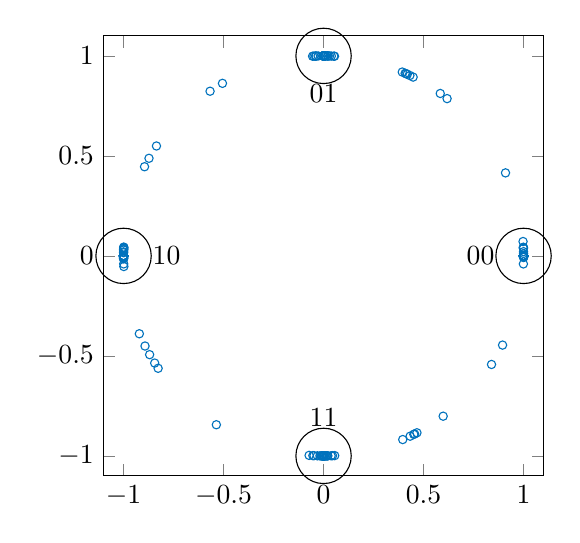
\begin{tikzpicture}

\begin{axis}[%
width=2.2in,
height=2.2in,
%at={(0.745in,1.046in)},
scale only axis,
xmin=-1.1,
xmax=1.1,
ymin=-1.1,
ymax=1.1,
axis background/.style={fill=white},
%axis x line*=bottom,
%axis y line*=left
]
\addplot[only marks,mark=o,mark options={},mark size=1.5000pt,color=mycolor1] plot table[row sep=crcr]{%
1	0\\
0	1\\
1	0\\
0	1\\
-1	0\\
1	0\\
0.451354373123749	-0.892344793150085\\
0.418635713079533	0.908154248866563\\
-0.999904228201287	-0.013839596279834\\
-0.00278951474474304	0.999996109296176\\
-0.0270468471608167	0.999634167112479\\
-0.0478868980007685	-0.9988527644252\\
-0.998587970431368	-0.0531231146466448\\
0.0202878243494571	0.999794180910834\\
-0.999573839713221	0.0291914193037453\\
0.0194263614182157	-0.999811290435375\\
-0.999971624448346	-0.00753327937466808\\
-0.999195866842604	0.0400951329297773\\
-0.0395891387431115	0.999216042752306\\
-0.921125436607137	-0.389265886041035\\
-0.895133012418738	0.445799158902476\\
-1	0\\
0	1\\
-0	1\\
1	0\\
1	0\\
0	-1\\
-1	0\\
-1	-0\\
-1	0\\
0	-1\\
0	-1\\
-1	0\\
0	-1\\
-0.892734663934763	-0.450582755783314\\
0.412537695936089	0.910940530129022\\
-0.00131558305931127	0.999999134620233\\
-0.0391404404091591	0.999233719369286\\
0.0548501509871476	0.998494597349774\\
0.997412994835308	0.0718840575765058\\
-0.99910744284425	0.0422411843255237\\
0.999982395445475	-0.00593370028994364\\
-0.0308237820817037	-0.999524834337887\\
-0.0548320921221509	0.998495589210843\\
-0.0179562264581751	-0.999838773968775\\
-0.00165277433412926	0.999998634167568\\
-0.99979896842517	0.020050504631197\\
0.395924129092239	-0.918283226462594\\
0.431608832539165	0.902060871379631\\
1	0\\
0	1\\
-1	0\\
1	0\\
1	0\\
-1	0\\
1	0\\
0	-1\\
0	1\\
-0	1\\
0	-1\\
1	0\\
-0	-1\\
0.455310295113608	-0.89033282269248\\
0.408015985508368	0.912974783643905\\
0.00290147235631477	-0.999995790720224\\
0.0134618671852259	-0.999909384960401\\
0.0298994322965629	0.999552912030345\\
0.9999947303803	0.0032464151969781\\
-0.0480345332129346	0.998845675577071\\
0.999195506258723	-0.0401041178979701\\
0.0106450314564717	0.99994334004747\\
0.0557291416079938	-0.998445923811418\\
-0.0722210874950609	-0.997388647680046\\
0.999077937733199	0.0429333708760311\\
0.0513646140446977	0.998679966968417\\
0.432979223844142	-0.90140390043494\\
0.895043035745952	-0.445979779993074\\
0	-1\\
0	1\\
1	0\\
-1	0\\
-0	1\\
1	0\\
-1	0\\
1	0\\
-0	-1\\
1	0\\
1	0\\
0	-1\\
-1	0\\
0.46682323850437	-0.884350645384675\\
0.393602108520103	0.919280903841981\\
-0.999035512596453	0.0439095043372386\\
0.00681407862108461	0.999976783896779\\
0.999087627930469	0.0427072794294872\\
0.999967835188107	-0.00802051053306116\\
0.00826886670098629	0.999965812337343\\
-0.999874731472365	0.0158278666618784\\
-0.999899601674204	-0.0141699178462274\\
0.0213278316445863	-0.999772535928718\\
-0.00857274663351669	-0.99996325333242\\
-0.99949875893509	0.0316580303748487\\
0.90978409190399	0.415081806537497\\
0.447805295980828	0.894131096032077\\
-0	1\\
0	1\\
0	1\\
-1	0\\
0	1\\
-0	1\\
0	1\\
1	0\\
1	0\\
0	1\\
1	0\\
1	0\\
-1	0\\
1	0\\
-0.50549373682538	0.862830274173498\\
-0.872842983618106	0.488001153634542\\
0.999778495649987	0.0210466062786834\\
0.999926613937712	0.0121147323149204\\
0.0377465332820373	-0.9992873456745\\
-0.999334635602086	0.0364730871471922\\
0.0115195372888084	-0.999933647929027\\
0.0388094138896332	0.999246630914282\\
0.0447653786826112	-0.998997527960606\\
0.022770068220817	0.999740728385725\\
-0.869597742768225	-0.493760838637906\\
-0.536016671359103	-0.844207396334045\\
1	0\\
-0	1\\
0	-1\\
1	0\\
1	-0\\
-1	0\\
1	0\\
0	1\\
1	0\\
-1	0\\
1	0\\
0	1\\
0	-1\\
0	-1\\
1	0\\
-0	-1\\
0	1\\
-0.827172347447776	-0.561948314009158\\
0.839827645780463	-0.542853134266392\\
0.999298327196063	0.0374546827933371\\
-0.0107915093990346	-0.999941769967077\\
-0.999990456870847	-0.00436877182230573\\
0.00489467474535381	-0.99998802100782\\
0.0108832274017805	0.999940775926915\\
-0.999954883753598	-0.00949897138266539\\
-0.844308169408405	-0.535857924332774\\
0.583460417950854	0.812141576749162\\
1	0\\
1	0\\
1	0\\
0	1\\
1	0\\
0	1\\
0	-1\\
1	0\\
0	1\\
-0	1\\
1	0\\
-0	-1\\
-1	0\\
-0	1\\
1	0\\
-1	0\\
1	0\\
0	1\\
0	1\\
0.598060955043327	-0.801450618598965\\
-0.835454637922525	0.549559412596802\\
0.0206450107654854	0.999786869052846\\
-0.999198472947712	-0.0400301343859802\\
-0.053481302595798	-0.998568851042659\\
-0.0371885137148704	0.999308267977244\\
-0.567491373991973	0.823379341764598\\
0.617675281880798	0.786433243291175\\
1	0\\
-1	0\\
-1	0\\
-1	0\\
0	-1\\
-1	0\\
0	-1\\
0	-1\\
-0	-1\\
0	1\\
-1	0\\
0	1\\
-0	-1\\
0	-1\\
0	-1\\
0	1\\
};
\end{axis}
\draw (1.1in,0.1in) circle (10pt) node [above=7pt] {11};
\draw (1.1in,2.1in) circle (10pt) node [below=7pt] {01};
\draw (2.1in,1.1in) circle (10pt) node [left=7pt] {00};
\draw (0.1in,1.1in) circle (10pt) node [right=7pt] {10};
\end{tikzpicture}%
	}
\end{minipage}	
\begin{minipage}{0.45\textwidth}
	\centering
	\subfigure[DSSS星座图]{
		% This file was created by matlab2tikz.
%
%The latest updates can be retrieved from
%  http://www.mathworks.com/matlabcentral/fileexchange/22022-matlab2tikz-matlab2tikz
%where you can also make suggestions and rate matlab2tikz.
%
\definecolor{mycolor1}{rgb}{0.00000,0.44700,0.74100}%
%
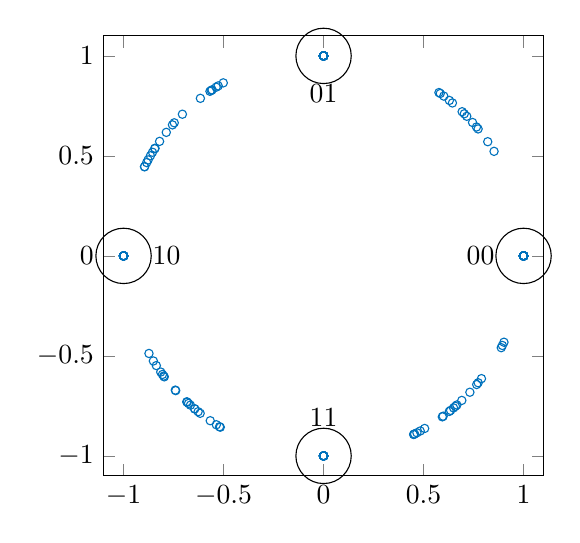
\begin{tikzpicture}

\begin{axis}[%
width=2.2in,
height=2.2in,
%at={(0.745in,5.553in)},
scale only axis,
xmin=-1.1,
xmax=1.1,
ymin=-1.1,
ymax=1.1,
axis background/.style={fill=white},
%axis x line*=bottom,
%axis y line*=left
]
\addplot[only marks,mark=o,mark options={},mark size=1.5000pt,color=mycolor1] plot table[row sep=crcr]{%
1	0\\
0	1\\
-1	0\\
1	0\\
1	0\\
1	0\\
0.451354373123749	-0.892344793150085\\
0.483477042464195	-0.875357041103843\\
-0.526775473680962	0.850004470769536\\
0.820922277888439	0.571039940517698\\
0.772649743577538	0.634832555678711\\
0.659314195195082	-0.751867536215164\\
0.692989500433354	0.720947676526619\\
-0.644717809043198	-0.764420660829192\\
-0.616961743457272	-0.786993142988021\\
-0.819836539479824	0.572597632315876\\
-0.520069296620092	-0.85412406985934\\
-0.865674975992414	0.500606468136932\\
-0.895133012418738	0.445799158902476\\
1	0\\
1	0\\
-1	0\\
0	1\\
0	1\\
0	1\\
0	1\\
1	0\\
0	1\\
1	0\\
0	1\\
0	1\\
1	0\\
0	1\\
0	1\\
0.450582755783314	-0.892734663934763\\
-0.872940729774165	-0.48782628291365\\
-0.850903570427007	-0.525321914481559\\
0.593772552517712	-0.80463293238383\\
-0.615884008652706	0.787836840904177\\
0.69125320584306	-0.722612624724819\\
0.73161125759851	-0.681722060487357\\
0.765751701695583	-0.643136324079366\\
-0.62715002521831	-0.778898482389504\\
-0.56656481595942	-0.824017177804485\\
-0.855267011732131	0.518187551609252\\
-0.884452443060157	0.466630341882007\\
0.902060871379631	-0.431608832539165\\
0	1\\
0	-1\\
0	1\\
1	0\\
0	1\\
-1	0\\
0	-1\\
-1	0\\
0	1\\
0	-1\\
-1	0\\
-1	0\\
0	1\\
1	0\\
-1	0\\
0.455310295113608	-0.89033282269248\\
-0.501352769987196	0.865242971671059\\
-0.836186433733103	-0.54844530086483\\
-0.796502151920223	-0.604635693609345\\
0.63515493223274	-0.772384756491493\\
0.74493681503282	0.667135025020242\\
-0.681814340066511	-0.731525259768703\\
0.644336027559505	0.764742494954241\\
0.789553828589112	-0.61368131123595\\
-0.844311861114489	0.535852107564567\\
-0.516366539697346	-0.85636767610705\\
0.888494681863551	-0.458886914500933\\
-0.895043035745952	0.445979779993074\\
0	-1\\
1	0\\
1	0\\
0	1\\
-1	0\\
0	1\\
0	1\\
0	1\\
0	-1\\
0	1\\
-1	0\\
0	-1\\
1	0\\
1	0\\
-1	0\\
0.466823238504371	-0.884350645384675\\
-0.536971991496216	0.84360007133036\\
-0.567995601992507	0.823031588772369\\
-0.80538057174272	-0.592758074309721\\
0.650019471328135	-0.759917552695219\\
0.716014235586821	0.698085678435692\\
-0.675199043083239	-0.737635582262324\\
-0.644387188500101	-0.764699386227644\\
0.60122910199349	0.799076696516737\\
-0.842695660662732	0.538390214900125\\
-0.877301563979607	0.479939543941668\\
0.894131096032077	-0.447805295980828\\
-1	0\\
0	1\\
0	1\\
-1	0\\
1	0\\
1	0\\
0	1\\
0	-1\\
-1	0\\
0	1\\
1	0\\
1	0\\
1	0\\
1	0\\
-1	0\\
1	0\\
0.50549373682538	-0.862830274173498\\
0.852467044401961	0.522780965805552\\
-0.557452376091253	0.830208918520041\\
-0.799320341388124	-0.600905143798231\\
-0.741356081817296	-0.671111883334297\\
0.703631511562309	0.710565053979254\\
-0.755498119974916	0.655150815243611\\
0.773096194403866	-0.634288794003379\\
0.576969862916365	0.816765435903278\\
-0.536016671359103	-0.844207396334045\\
0	-1\\
-1	0\\
0	1\\
0	1\\
1	0\\
0	-1\\
-1	0\\
0	-1\\
1	0\\
-1	0\\
1	0\\
1	0\\
1	0\\
0	1\\
0	1\\
1	0\\
0	-1\\
0	1\\
1	0\\
-0.561948314009158	0.827172347447776\\
-0.81408296357137	-0.580748593130329\\
0.628808591471087	-0.777560129695541\\
0.66657179468931	-0.745440837709253\\
-0.705798388005434	0.708412757853027\\
-0.665678715079009	-0.746238466102331\\
0.629137091304567	0.777294358878816\\
0.583460417950854	0.812141576749162\\
0	-1\\
-1	0\\
0	1\\
1	0\\
0	-1\\
0	-1\\
0	-1\\
1	0\\
1	0\\
1	0\\
0	1\\
0	-1\\
0	1\\
-1	0\\
0	1\\
0	1\\
0	1\\
0	-1\\
0	1\\
1	0\\
1	0\\
0.598060955043327	-0.801450618598965\\
0.764634571169287	0.64446409719453\\
-0.739197401062536	-0.673488828609942\\
-0.684006436199114	-0.729475973036938\\
-0.74643307944447	0.665460485612066\\
-0.786433243291175	0.617675281880798\\
0	-1\\
0	1\\
0	-1\\
0	-1\\
0	1\\
0	1\\
1	0\\
0	1\\
0	1\\
1	0\\
-1	0\\
0	1\\
-1	0\\
1	0\\
0	1\\
0	1\\
1	0\\
1	0\\
nan	nan\\
};
\end{axis}
\draw (1.1in,0.1in) circle (10pt) node [above=7pt] {11};
\draw (1.1in,2.1in) circle (10pt) node [below=7pt] {01};
\draw (2.1in,1.1in) circle (10pt) node [left=7pt] {00};
\draw (0.1in,1.1in) circle (10pt) node [right=7pt] {10};
\end{tikzpicture}%
	}
\end{minipage}
\caption{$\alpha=10^{-4}$时DDSS和DSSS星座图对比}
\label{fig:software:scatter}
\end{figure}

图\ref{fig:software:dp1}给出了在不同多普勒情况下DDSS系统和DSSS系统的误码率曲线。可以看出,在没有进行任何多普勒补偿的DSSS系统几乎完全无法正确接收数据。而引入了二阶差分的DDSS系统,在一定程度上消除了多普勒的影响。
\begin{figure}[!htbp]
	\centering
	% This file was created by matlab2tikz.
%
%The latest updates can be retrieved from
%  http://www.mathworks.com/matlabcentral/fileexchange/22022-matlab2tikz-matlab2tikz
%where you can also make suggestions and rate matlab2tikz.
%
\definecolor{mycolor1}{rgb}{0.00000,0.44700,0.74100}%
\definecolor{mycolor2}{rgb}{0.85000,0.32500,0.09800}%
\definecolor{mycolor3}{rgb}{0.520000,0.22700,0.44100}%
%
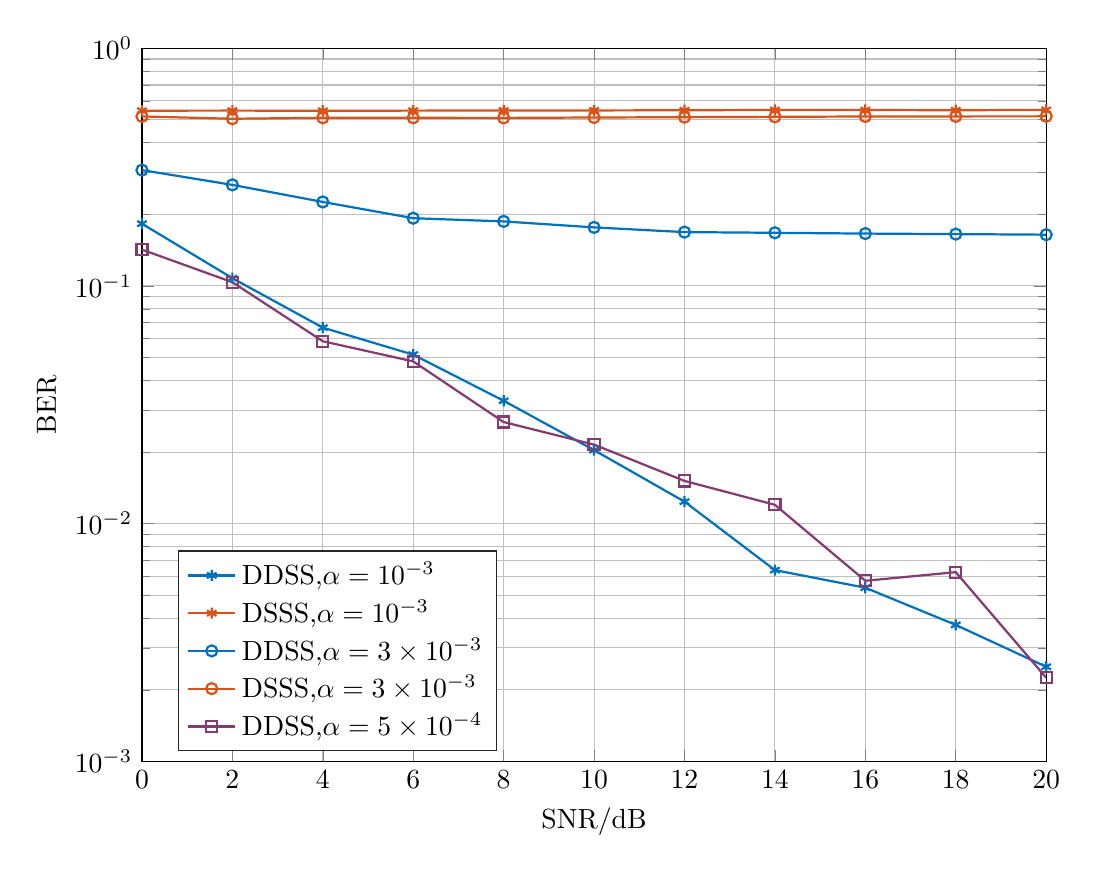
\begin{tikzpicture}

\begin{axis}[%
width=4.521in,
height=3.566in,
at={(0.758in,0.481in)},
scale only axis,
xmin=0,
xmax=20,
xlabel={SNR/dB},
xmajorgrids,
ymode=log,
ymin=0.001,
ymax=1,
yminorticks=true,
ylabel={BER},
ymajorgrids,
yminorgrids,
axis background/.style={fill=white},
legend style={at={(0.04,0.014)},anchor=south west,legend cell align=left,align=left,draw=white!15!black}
]
\addplot [color=mycolor1,line width=0.8pt,solid,mark=asterisk,mark options={solid}]
  table[row sep=crcr]{%
0	0.182625\\
2	0.10775\\
4	0.06675\\
6	0.051375\\
8	0.032875\\
10	0.020375\\
12	0.012375\\
14	0.006375\\
16	0.005375\\
18	0.00375\\
20	0.0025\\
};
\addlegendentry{DDSS,$\alpha=10^{-3}$};

\addplot [color=mycolor2,line width=0.8pt,solid,mark=asterisk,mark options={solid}]
  table[row sep=crcr]{%
0	0.54575\\
2	0.54625\\
4	0.54525\\
6	0.546125\\
8	0.546625\\
10	0.547125\\
12	0.548\\
14	0.5495\\
16	0.549375\\
18	0.548125\\
20	0.54975\\
};
\addlegendentry{DSSS,$\alpha=10^{-3}$};

\addplot [color=mycolor1,solid,line width=0.8pt,mark=o,mark options={solid}]
table[row sep=crcr]{%
	0	0.307\\
	2	0.266\\
	4	0.2255\\
	6	0.192625\\
	8	0.18675\\
	10	0.17625\\
	12	0.168375\\
	14	0.16725\\
	16	0.166\\
	18	0.165125\\
	20	0.16425\\
};
\addlegendentry{DDSS,$\alpha=3\times10^{-3}$};

\addplot [color=mycolor2,solid,mark=o,line width=0.8pt,mark options={solid}]
table[row sep=crcr]{%
	0	0.516125\\
	2	0.50475\\
	4	0.5095\\
	6	0.509375\\
	8	0.508875\\
	10	0.510875\\
	12	0.5125\\
	14	0.51425\\
	16	0.515875\\
	18	0.516375\\
	20	0.516625\\
};
\addlegendentry{DSSS,$\alpha=3\times10^{-3}$};

\addplot [color=mycolor3,solid,line width=0.8pt,mark=square,mark options={solid}]
table[row sep=crcr]{%
	0	0.142125\\
	2	0.103625\\
	4	0.0585\\
	6	0.048125\\
	8	0.02675\\
	10	0.0215\\
	12	0.015125\\
	14	0.012\\
	16	0.00575\\
	18	0.00625\\
	20	0.00225\\
};
\addlegendentry{DDSS,$\alpha=5\times10^{-4}$};

\end{axis}
\end{tikzpicture}%
	\caption{DDSS和DSSS仿真误码率}
	\label{fig:software:dp1}
\end{figure}

\section{MSP432驱动软件设计}
%	MSP432驱动程序包括ADC数据采集驱动和UART数据传输驱动两部分。
%在设计驱动程序时参考了中断-回调函数模型,即中断服务函数处理中断请求然后请求调用
%回调函数。回调函数不是由中断服务函数直接调用,而是由中断服务函数连接到回调函数链表中由
%主函数根据优先级决定执行哪个回调函数。
\subsection{设备驱动模型}
本文结合linux驱动架构,设计实现了一个设备-驱动的驱动程序模型。模型将外设驱动程序分为设备层和驱动层,设备层描述msp432具体的外设模块,驱动层描述对外设模块的操作。例如msp432中的uart0和uart1是不同的设备,但它们都对应一个驱动。设备由
msp432\_dev结构体描述,驱动由结构体msp432\_driver描述,它们的定义如下:
\begin{lstlisting}
typedef struct msp432_dev_t {
	void *phy_addr;
	uint16_t flag;
	void *prvt;
} msp432_dev;

void msp432_dev_init(msp432_dev *dev,
                     void *phy_addr,
                     uint16_t flag, 
                     void *privte);
typedef struct msp432_driver_t {
	int (*open)(msp432_dev *dev,int16_t mode);
	int (*close)(msp432_dev *dev);
	int (*write)(msp432_dev *dev,void *buf, size_t count);
	size_t (*read)(msp432_dev *dev,void *buf, size_t count);
	int (*ioctl)(msp432_dev *dev,int16_t key, int16_t val);
	void (*interp)(msp432_dev *dev,void *p);
} msp432_driver;
\end{lstlisting}
其中,msp432\_dev描述关于设备的物理地址(phy\_addr)、状态或标志(flag)和私有数据;msp432\_driver描述关于的设备操作,open、close、write、read四个函数指针为操作设备的函数入口,interp函数指针为中断下部处理入口,其参数p为中断上部传入的私有数据。需要指出的是,中断服务(isr)函数属于设备层,中断下部属于驱动层。以上定义了驱动程序的模型,根据这一模型编写设备驱动的方法将更加标准化。下面以UART模块为例,简要介绍如何利用驱动模型编写驱动。
\begin{lstlisting}
/*file:msp432_uart.c*/ 
#include “**.h” //包含必要的头文件

/*UART设备打开函数*/
int uart_open()
{
	// 配置UART,成功返回0,失败返回负值
}

/*UART关闭、读、控制等函数*/
int uart_close()
{
	//关闭USART
}

int uart_read()
{
	//读取数据
}

int uart_ioctl()
{
	//控制采样率等
}

int uart_write()
{
	//写入数据
}
//interp函数为回调函数在中断服务函数中调用
/*UART中断服务函数*/
void uart_interrupt()
{
	//处理中断,回调interp
}

//定义设备操作
msp432_driver msp432_uart_driver={
	.open=uart_open,
	.close=uart_close,
	.write=uart_write,
	.read=uart_read,
	.ioctl=uart_ioctl,
	.interp=null,
};

//定义并初始化UART设备
unsigned char buf0[BUFF_SIZE];//数据缓存
unsigned char buf1[BUFF_SIZE];//数据缓存
msp432_dev msp432_uart0,msp432_uart1;

//初始化UART0,将buf0作为私有数据给UART0
msp432_dev_init(&msp432_uart0,UART0_ADDR,0,(void *)buf0);

//初始化UART1,将buf1作为私有数据给UART1
msp432_dev_init(&msp432_uart1,UART1_ADDR,0,(void *)buf1);
\end{lstlisting}

%open函数只做与当前模块有关的初始化,部操作其他模块。例如,UART工作时,还需要Timer\_A0为其提供时钟,Timer\_A0的操作需在UART打开之前完成。open函数根据dev参数决定初始化哪一个设备,并将初始化后的状态写入dev->flag中。open可以将设备打开为阻塞或者费非阻塞、只读只写或者可读可写等,这受mode参数控制。
%
%在阻塞的情况下,write将buf中的数据逐字发送然后返回,read则等待读入count比特数据后再返回;在非阻塞情况下,则交由中断函数处理。
%
%msp432\_dev\_init将缓存地址给msp432\_dev的私有数据指针,当uart的read函数被调用时可以通过read函数传进的dev参数获取缓存的地址并读出数据。

下面,将详细介绍不同模块基于设备-驱动模型的编写实例。

\subsection{UART驱动模块}
\begin{figure}[!htbp]
	\centering
	
\tikzstyle{comment}=[rectangle, draw=black, rounded corners, fill=gray!10,
text centered, anchor=north, text width=3cm]

\begin{tikzpicture}
  \node (uart0) [comment, rectangle split, rectangle split parts=2, text justified,text width=4cm]
  {
  	\textbf{uart0:msp432\_dev}
  	\nodepart{second}phy\_addr:EUSCI\_A0\newline flag:\newline privt:\&p
  };
  
  \node (uart-driver) [comment, rectangle split, rectangle split parts=2, text justified,text width=5cm,below = 6cm of uart0.west,anchor=west] 
  {
  	\textbf{uart\_driver:msp432\_driver}
  	\nodepart{second}open:uart\_open\newline close:uart\_close \newline read:uart\_read \newline write:uart\_write \newline ioctl:uart\_ioctl \newline interpt:uart\_interpt
  };
  
  \node (private) [comment, rectangle split, rectangle split parts=2, text justified,text width=4cm,right = 6cm of uart0.north,anchor=north]
  {
  	\textbf{p:uart\_dev\_private}
  	\nodepart{second}sendbuf\newline recvbuf \newline sendidx \newline recvidx \newline sendlen \newline recvlen
  };
  
  \node (code) [comment, text justified,text width=4cm,right = 6cm of uart-driver.north,anchor=north,yshift=-1cm]
  {
  	uart\_open()\\
  	$~~~~~~$$\vdots$\newline
  	uart\_interpt()
  	
  };
  
  \draw [-,dashed,line width=0.35mm] (-3.0cm,0.5cm) --+(0,-10cm);
  \draw [dashed,line width=0.35mm] (-3.0cm,-4.3cm) --+ (11.5cm,0);
  
  \node at (-3.8cm,-3cm) {应用层};
  \node at (-2.2cm,-3.6cm) {设备层};
  \node at (-2.2cm,-5cm) {驱动层};
   
  
  
\end{tikzpicture}
	\caption{UART模块结构图}
	\label{fig::software:uart}
\end{figure}
UART设备层程序中声明了类型为msp432\_dev的全局变量uart0和设备私有数据结构变量p,uart0将作为全局设备访问uart0。设备的私有数据为数据缓存结构,包含缓存的首地址、缓存大小的缓存计数。在模块初始化函数中,首先初始化了私有数据结构p,然后将p的地址给uart0的prvt成员。用UART0的物理首地址初始化uart0的phy\_addr成员,并将uart0的flag成员初始化为0。模块的退出函数释放缓存并关闭设备。

模块还引用了类型为msp432\_driver的msp432\_uart\_driver。在模块定义的uart0的中断服务函数中调用msp432\_uart\_driver的interp中断下部函数。

在UART驱动层程序中实现了驱动操作函数的打开、关闭、读数据、写数据及中断下部函数。中断下部函数将接受数据存入接受缓存中,从发送缓存中取出数据发送出去。UART驱动的ioctl函数用于设置数据位、校验为停止位等传输格式。

图\ref{fig::software:uart}为UART模块的结构关系,图中以三个结构体为主线索展示了模块结构。其中msp432\_dev和msp432\_driver为驱动模型顶层的结构,uart\_dev\_private为UART模块私有的结构。对于应用程序来说,只需通过msp432\_dev和msp432\_driver就可以操作模块。


%	UART驱动设计为1152008N1(波特率115200bps,8位数据位,无校验位,1位停止位)传输格式。UART的接受
%采用中断-回调函数模型,回调函数形式为:void msp432\_uart\_callback(uint16\_t *data, uint32\_t len)。在UART中断服务函数中判断如果是接收中断,则将UART接收缓冲区的数据拷贝至接收缓存。UART接受缓冲区位于UART模块内,MSP432内核可以通过外设地址映射来访问它;接收缓存位于内存中,是程序定义的数组缓存。如果接收缓存满且回调函数指针不为null时调用回调函数。回调函数的data参数为内存中接收缓存的首地址,len参数为接收缓存的长度。
%
%	UART的发送利用$\mu$DMA以实现非阻塞调用。提供给的外部编程接口为函数int msp432\_uart\_send(uint8\_t *data, uint32\_t len)
%,函数将数据存入缓存区域并启动$\mu$DMA通道,函数返回实际写入缓存区域的数据长度,如果写入失败则返回-1。UART模块的发送缓冲区为空时,会将UART的发送中断标志位置1。发送中断标志为触发$\mu$DMA对应的通道将待发送的缓存数据转移至UART的发送缓冲区。UART逐bit将发送缓冲区的数据发送出去后,再次将发送中断标志位置1。以此类推,当$\mu$DMA将全部缓存数据转移完毕之后则关闭该$\mu$DAM通道,等待下一次缓存数据到来。 
\subsection{ADC驱动模块}
ADC驱动模块与UART模块结构相似,只是私有数据结构不一样。本节只给出结构图和私有数据结构定义,不在赘述其架构原理。
\begin{figure}[!htbp]
	\centering
	
\tikzstyle{comment}=[rectangle, draw=black, rounded corners, fill=gray!10,
text centered, anchor=north, text width=3cm]

\begin{tikzpicture}
  \node (adc0) [comment, rectangle split, rectangle split parts=2, text justified,text width=4cm]
  {
  	\textbf{adc0:msp432\_dev}
  	\nodepart{second}phy\_addr:ADC\_MEM0 \newline flag:\newline privt:null
  };
  
  \node (adc-driver) [comment, rectangle split, rectangle split parts=2, text justified,text width=5cm,below = 6cm of adc0.west,anchor=west] 
  {
  	\textbf{adc\_driver:msp432\_driver}
  	\nodepart{second}open:adc\_open\newline close:adc\_close \newline read:adc\_read \newline write:adc\_write \newline ioctl:adc\_ioctl \newline interpt:adc\_interpt
  };
  
  
  \node (code) [comment, text justified,text width=4cm,right = 6cm of adc-driver.north,anchor=north,yshift=-1cm]
  {
  	adc\_open()\\
  	$~~~~~~$$\vdots$\newline
  	adc\_interpt()
  	
  };
  
  \draw [-,dashed,line width=0.35mm] (-3.0cm,0.5cm) --+(0,-10cm);
  \draw [dashed,line width=0.35mm] (-3.0cm,-4.3cm) --+ (11.5cm,0);
  
  \node at (-3.8cm,-3cm) {应用层};
  \node at (-2.2cm,-3.6cm) {设备层};
  \node at (-2.2cm,-5cm) {驱动层};
   
  
  
\end{tikzpicture}
	\caption{ADC模块结构图}
	\label{fig::software:adc}
\end{figure}

\subsection{DMA驱动模块}
考虑到DMA的复杂性,DMA模块将不使用设备驱动模型。本文只使用了DMA的通道7的ping-pong模式用于ADC数据采集。

模块首先在RAM中定义了两个ping-pong缓存数据区。然后初始化通道7的主传输通道,用ADC触发通道7的单次循环传输。在DMA的中断中判断,如果是通道7主传输通道传输完毕则初始化通道7的副传输通道;如果是通道7副传输通道传输完毕则初始化通道7的主传输通道。然后调用DMA的回调函数。回调函数可以指向任何需要ADC采集数据的目标函数。
%	% 流程图定义基本形状
%	\tikzstyle{startstop} = [rectangle, rounded corners, minimum width=3cm, minimum height=1cm,text centered, draw=black]
%	\tikzstyle{io} = [trapezium, trapezium left angle=40, trapezium right angle=140, minimum width=3cm, minimum height=1cm, text centered, draw=black]
%	\tikzstyle{process} = [rectangle, minimum width=3cm, minimum height=1cm, text centered, draw=black]
%	\tikzstyle{decision} = [diamond, minimum width=3cm, minimum height=1cm, text centered, draw=black,aspect=2]
%	\tikzstyle{arrow} = [thick,->,>=stealth]
%	\begin{figure}[htbp]
%		\centering
%		\begin{tikzpicture}[node distance=1.5cm]
%		%定义流程图具体形状
%		\node (start) [startstop] {中断触发};
%		\node (dec1) [decision, below of=start, yshift=-1.0cm] {是否PING中断};
%		\node (dec2) [decision, below of=dec1, yshift=-1.5cm] {是否PONG中断};
%		\node (pro1) [process, right of=dec2, xshift=3.0cm] {请求回调};
%		\node (return) [startstop, below of=dec2,yshift=-1.5cm] {返回};
%		\path node(fake) [right of=pro1]{};
%		
%		
%		%连接具体形状
%		\draw [arrow](start) -- (dec1);
%		\draw [arrow](dec1) -| node[anchor=south] {是} (pro1);
%		\draw [arrow](dec1) -- node[anchor=east] {否} (dec2);
%		
%		\draw [arrow](dec2) -- node[anchor=north] {是} (pro1);
%		\draw [arrow](dec2) -- node[anchor=east] {否} (return);
%		
%		\draw [arrow](pro1) |-  (return);
%		\end{tikzpicture}
%		\caption{ADC数据采集驱动流程图}
%		\label{Figure:Software:ADCModule}
%	\end{figure}
%	系统采用带通采样以降低数据处理负荷,采样率$4kHz$。MSP432的Timer\_A0为ADC14提供采样率
%的采样保持时钟。为保证系统实时性,采集数据设计为PING-PONG存储。MSP432的$\mu$DMA模块提供这一功能。
%PING-PONG大小为$2\times1024$存储单元。每采集完成一次PING-PONG即触发一次中断,在中断服务函数中判断
%是PING还是PONG,然后请求调用回调函数。
%
%	回调函数的形式为:void msp432\_adc14\_callback(uint16\_t *data, uint32\_t len)。
%参数data为当前完成采集的存储区的首地址,参数len为存储区大小。图\ref{Figure:Software:ADCModule}为ADC数据采集驱动的流程图。

\section{MSP432动态内存管理}
	单片机在做信号处理算法时常常遇到需要使用较大数组的问题。例如在做32bit浮点采样数据为900点,本地数据为108点的快速相关算法时
需要分配至少两个4k大小的存储区域。在编写函数时有三种处理方式:

\begin{publist}
	\item 使用全局变量静态分配内存,存储区位于静态数据区。这样做的好处是分配内存在程序编译阶段就已经做好,但是内存永久占用不能释放,而且对于内存较小的
	单片机来说,分配较多的大块内存将带来大量内存的消耗;
	\item 使用局部变量,存储区位于栈内。这样做可以函数调用完之后内存可以释放,可以缓解静态分配内存的问题。但是如果遇到函数多次嵌套调用可能会导致栈益处;
	\item 使用malloc动态分配内存,存储区位于堆内。这样做可以解决静态分配和局部变量动态分配的所有问题,但是c标准库中的malloc函数算法复杂,分配与释放
	很耗时,而且需要链接较大的标准库的代码使程序体积增大。
\end{publist}

	信号处理算法虽然需要较多的大块内存,但是所有的内存大小几乎都一致即对某个固定大小的内存需求较多。针对这一前提,并结合动态内存分配的内存池算法重新实现了
快速的动态内存管理。


\subsection{内存池介绍}
	内存池(Memory Pool),又被称为固定大小区块规则(fixed-size-block allocation),允许程序设计者以类似C语言的malloc或者C++的new运算符进行动态内存的申请。
对于其他动态内存分配算法来说,因为会动态记忆区块大小导致的碎片问题,致使在实时系统上表现不佳,甚至根本无法使用。
内存池技术提供了一种更有效率的解决方案:预先规划一定数量的内存区块,使程序可以在执行期分配(allocate)、使用(access)和释放(free)内存区块。
	
	图\ref{Figure:Software:memalloc}为以内存池实例,内存池包含4个1k大小、2个2k大小和1个4k大小的内存块。图\ref{Figure:Software:memalloc}还展示了多次分配内存的过程:
	
\begin{publist}
	\item 请求一个大小为4k的内存快,此时内存池匹配到第一个大小为2k的内存区域;
	\item 请求4个大小都为1k的内存快,此时内存池分别匹配到4个大小为1k的内存区域,至此大小为1k的内存块用尽;
	\item 再次请求一个大小为1k的内存块,此时内存池将在2k大小的池内匹配内存区域
	\item 如果再请求1k或者2看的内存块,内存池将在4k大小的池内匹配内存区域。
\end{publist}

	\begin{figure}[htbp]
		\centering
		\def \nod{~~~~}
\def \zihao{\wuhao}
	\tikzstyle{neuron}=[circle,fill=black!25,minimum size=0pt,inner sep=0pt]
	\tikzstyle{num}=[circle,fill=red!25,minimum size=0pt,inner sep=0pt]

\begin{tikzpicture}[>=stealth',node distance=1cm]
	\draw 
		(0,0) rectangle ++(1,1)
		(1,0) rectangle ++(1,1)
		(2,0) rectangle ++(1,1)
		(3,0) rectangle ++(1,1)
		(4,0) rectangle ++(2,1)
		(6,0) rectangle ++(2,1)
		(8,0) rectangle ++(4,1)
		;
	\draw 
		(0.5,0.5) node {1k}
		++(1,0) node {1k}
		++(1,0) node {1k}
		++(1,0) node {1k}
		++(1.5,0) node {2k}
		++(2,0) node {2k}
		++(3,0) node {4k}
	;

	\draw[yshift=-1.5cm] 
		(0,0) rectangle ++(1,1)
		(1,0) rectangle ++(1,1)
		(2,0) rectangle ++(1,1)
		(3,0) rectangle ++(1,1)
		(4,0) rectangle ++(2,1)
		(6,0) rectangle ++(2,1)
		(8,0) rectangle ++(4,1)
	;
	\draw[yshift=-1.5cm,fill=gray!20] (4,0) rectangle ++(2,1);
	
	\draw[yshift=-3cm] 
		(0,0) rectangle ++(1,1)
		(1,0) rectangle ++(1,1)
		(2,0) rectangle ++(1,1)
		(3,0) rectangle ++(1,1)
		(4,0) rectangle ++(2,1)
		(6,0) rectangle ++(2,1)
		(8,0) rectangle ++(4,1)
	;
	\draw[yshift=-3cm,fill=gray!20]
		(0,0) rectangle ++(1,1)
		(1,0) rectangle ++(1,1)
		(2,0) rectangle ++(1,1)
		(3,0) rectangle ++(1,1)
		(4,0) rectangle ++(2,1)
	;
	
	\path[yshift=-4.5cm,fill=gray!20] (6,0) rectangle ++(1,1);
	\draw[yshift=-4.5cm] 
		(0,0) rectangle ++(1,1)
		(1,0) rectangle ++(1,1)
		(2,0) rectangle ++(1,1)
		(3,0) rectangle ++(1,1)
		(4,0) rectangle ++(2,1)
		(6,0) rectangle ++(2,1)
		(8,0) rectangle ++(4,1)
		;
	\draw[yshift=-4.5cm,fill=gray!20]
		(0,0) rectangle ++(1,1)
		(1,0) rectangle ++(1,1)
		(2,0) rectangle ++(1,1)
		(3,0) rectangle ++(1,1)
		(4,0) rectangle ++(2,1)
		;
	
	\draw node at (-1.cm,-1.cm) {\wuhao 分配2k};
	\draw[yshift=-1.5cm] node at (-1.4cm,-1.cm) {\wuhao 分配4个1k};
	\draw[yshift=-3cm] node at (-1.cm,-1.cm) {\wuhao 分配1k};
		
\end{tikzpicture}
		\caption{内存池内存分配实例}
		\label{Figure:Software:memalloc}
	\end{figure}

\subsection{内存池的优缺点}
	内存池允许在程序执行时以常数时间分配内存块,并且不会产生内存碎片。一次释放内存中大量空闲内存只需要一个操作,无需像malloc那样依次个别释放。
内存池不必将每次分配的内存的详细信息记录下来(例如内存大小,因为内存池本身就包含了大小的信息)。内存池在使用时也必须按照程序需求来做调整才能保证
时间与空间的效率,这也是内存池的显著缺点。

\subsection{内存池在本文中的应用}
	本文所涉及到的算法及所需要的内存大小如表\ref{Tab:Software:Tab1}所示。分析得出内存池需要最多1个32~Bytes,2个128Bytes,6个2048~Bytes和1个8192~Bytes的内存空间。
进一步分析,快速相关以及解调解扩相互间都是独立的,即前一算法执行完毕后一算法才会执行。因此,2048~Bytes的空间只需要2个。为给其他局部变量预留空间,最终的内存池分布为:
16~Bytes$\times$8、32~Bytes$\times$4、128~Bytes$\times$2、256~Bytes$\times$1、2048~Bytes$\times$2、4096~Bytes$\times$1、8192~Bytes$\times$1。


	\begin{table}[htbp]
		\centering 
		\caption{算法内存需求}
		\label{Tab:Software:Tab1}
		\vspace{0.5ex}
		\wuhao
		\begin{tabu} to \textwidth {X[1,c]|X[1,c]|X[1,c]|X[1,c]}
			\specialrule{1.5pt}{0pt}{0pt}
			% after \\: \hline or \cline{col1-col2} \cline{col3-col4} ...
			算法 & 		数据量 & 数据类型 & 占用空间(Byte) \\
			\hline
			快速相关& 	1024 $\times$ 2 & int16 & 2048 $\times$ 2 \\
			\hline
			\multirow{2}*{解调} & 2048$\times$2 & float32 & 8192$\times$2 \\
							& 512$\times$2  & float32 & 2048 $\times$2\\
			\hline
			\multirow{3}*{解扩与二阶差分检测} & 512 $\times$2 & float32 & 2048 $\times$ 2\\
							& 32 $\times$ 2 & float32 & 128 $\times$2 \\
							& 32 $\times$ 1 & int8 & 32 $\times$1 \\
			\specialrule{1.5pt}{0pt}{0pt}
		\end{tabu}
	\end{table}
	
\section{接收机程序设计}
接收机由MSP432完成,该部分程序主要实现DD-SS算法及数据流程控制,由同步、缓存、解扩三部分组成,它们之间的关系如图\ref{fig:software:ddss}所示。由ADC采集到的数据首先会进行同步搜索,搜索到同步信号后同步信号后的数据解调降采样后缓存。等到缓存满一帧后开始解扩及二阶差分检测,然后通过UART数据传输驱动将数据发出。
\begin{figure}[htbp]
	\centering
	\def \nod{~~~~}
\def \zihao{\wuhao}
	\tikzstyle{neuron}=[circle,fill=black!25,minimum size=0pt,inner sep=0pt]
	\tikzstyle{num}=[circle,fill=red!25,minimum size=0pt,inner sep=0pt]
	\tikzstyle{vecArrow} = [thick, decoration={markings,mark=at position
		1 with {\arrow[semithick]{open triangle 60}}},
	double distance=1.4pt, shorten >= 5.5pt,
	preaction = {decorate},
	postaction = {draw,line width=1.4pt, white,shorten >= 4.5pt}]
	\tikzstyle{adct} = [rectangle,fill=gray!25,minimum width=5cm, minimum height=1cm,text centered, draw=black]
	\tikzstyle{block} = [rectangle,fill=gray!75!red,minimum width=2cm, minimum height=1cm,text centered, draw=black]
\begin{tikzpicture}[>=stealth',node distance=3cm]
	\draw 
		node[adct] (adc) {ADC数据采集驱动}
		node[adct,xshift=6cm] (uart) {UART数据传输驱动}
		node[block,above of=adc,xshift=-1.5cm] (sync) {同步}
		node[block,right of=sync,xshift=1cm] (cache) {缓存}
		node[block,above of=uart] (pro) {解扩}
	;
	\node[inner sep=0,minimum size=0](hid) at (-1.5cm,0.5cm){};
	\node[inner sep=0,minimum size=0,right of=hid,xshift=-2.98cm,yshift=1cm](k) {};
	\draw [vecArrow] (hid) -- (sync);
	\draw [vecArrow] (k) -| (cache);
	\draw [vecArrow] (cache) -- (pro);
	\draw [vecArrow] (pro) -- (uart);
	\draw [vecArrow,dashed] (sync) -- (cache);
	
	\draw[dashed,very thick] (-4cm,1.0cm) --++(14cm,0);
	\node at (9.5cm,1.4cm) {应用层};
	\node at (9.5cm,0.6cm) {驱动层};
	
\end{tikzpicture}
	\caption{DD-SS程序组成框图}
	\label{fig:software:ddss}
\end{figure}

\subsection{同步搜索}
同步搜索采用双曲线调频信号(hyperbolic frequency-modulation,HFM)做相关进行。HFM是一种多普勒不变信号,其时间函数为\citeup{田坦2009声呐技术}
\begin{equation}
s(t)=Ae^{\left[-j\left(2\pi\frac{f_0^2}{m}\right)\ln\left(1-\frac{m}{f_0} t\right)\right]}
\end{equation}
频谱函数为\citeup{田坦2009声呐技术}
\begin{equation}
|S(f)|=A\frac{f_0}{\sqrt{|m|}\cdot f}
\end{equation}
图\ref{fig:software:hfm}展示了双曲线调频信号的幅度谱。
\begin{figure}[htbp]
	\centering
	\def \nod{~~~~}
\def \zihao{\wuhao}
\begin{tikzpicture}[>=stealth',node distance=3cm]
	\draw [->] (0,0) -- (6cm,0) node[below] {$f$};
	\draw [->] (0,0) -- (0,6cm) node[right] {$|S(f)|$};
	
	\draw[thick] plot[domain=1:5,samples=300,id=hfm] function{4.5/x};
	\draw[dashed] (1,0) -- (1,4.5)--(0,4.5);
	\draw[dashed] (3,0) -- (3,1.5)--(0,1.5);
	\draw[dashed] (5,0) -- (5,4.5/5)--(0,4.5/5);
	
	\node[left] at (0,4.5) {$\frac{Af_0}{\sqrt{|m|}f_L}$};
	\node[above left] at (0,1.5) {$\frac{A}{\sqrt{|m|}}$};
	\node[left] at (0,4.5/5) {$\frac{Af_0}{\sqrt{|m|}f_H}$};
	
	\node[below] at (1,0) {$f_L$};
	\node[below] at (3,0) {$f_0$};
	\node[below] at (5,0) {$f_H$};
	
	
	
\end{tikzpicture}
	\caption{双曲线调频信号幅度谱}
	\label{fig:software:hfm}
\end{figure}

由于HFM信号具有多普勒不变性\citeup{田坦2009声呐技术},即具有多普勒的接受信号$r(t)$与发射信号$s(t)$满足
\begin{equation}
r(t)=s(Dt)=s(t-t_0)
\end{equation}
式中,$D=1/\alpha\approx1+\delta$。可见,HFM将多普勒转化成为一个延时$t_0$,且
\begin{equation}
t_0=\frac{1-D}{(m/f_0)D}
\end{equation}

在MSP432的CMSIS-DSP库的直接相关算法计算速度慢,文献\cite{press2007numerical}介绍一种采用FFT的快速相关算法,利用快速相关算法可以节省大量运算时间。根据式(\ref{eq:ddcode:recv})可将接受信号写为
\begin{equation}
r(t)=\sum_{p=1}^{N_p}A_px(t-\tau_p)+n(t)
\end{equation}
式中$n(t)$为高斯白噪声,$x(t)$为HFM同步信号。经过相关后\citeup{farrokhi2008performance}
\begin{equation}
R_{rx}(\tau)=\sum_{p=1}^{N_p}A_pR_{xx}(\tau-\tau_p)+u(\tau)
\end{equation}
式中$u(\tau)$是噪声分量。$R_{rx}(\tau)$在$\tau_p(p=1,2,\cdots,N_p)$处有峰值,峰值$|A_p1R_{xx}(0)|$只与增益$A_p$有关。因此,选择峰值最大的第$q$个峰将得到最大的处理后信噪比。

\subsection{通带解调与缓存}
通带解调过程如图\ref{fig:software:pass}所示。I路与Q路分别乘以$\cos(\omega n)$和$\sin(\omega n)$后经过降采样滤波器得到时间宽度为$T_c$(扩频码宽度)的序列,然后缓存到缓存区。降采样滤波器将滤波和降采样结合,能够避免不必要计算的数据点大大节约了计算时间。缓存时,按照I路与Q路分开存储。
\begin{figure}[htbp]
	\centering
	
\begin{tikzpicture}[>=stealth']
		\tikzset{%
			block/.style    = {draw, thick, rectangle, minimum height = 2em,
				minimum width = 3em},
			sum/.style      = {draw, circle, inner sep=0pt, node distance = 2cm}, % Adder
			input/.style    = {coordinate}, % Input
			output/.style   = {coordinate} % Output
		}
		
		\node[input] (in) at(0,0) {};
		\node[sum] (t1) at (2,1) {\Large $\times$};
		\node[sum] (t2) at (2,-1) {\Large $\times$};
		\node[block,right of=t1,node distance = 2cm] (m1) {$\downarrow M$~FIR};
		\node[block,right of=t2,node distance = 2cm] (m2) {$\downarrow M$~FIR};
		\node[input,inner sep=0,minimum size=0] (f1) at(1,0) {};
		\draw (in) -- (f1);
		\draw[->] (f1) |- (t1);
		\draw[->] (f1) |- (t2);
		\draw[->] (t2) -- (m2);
		\draw[->] (t1) -- (m1);
		\draw node[above of=t1] (src1) {$\cos(\omega n)$};
		\draw[->] (src1)--(t1);
		
		\draw node[below of=t2] (src2) {$\sin(\omega n)$};
		\draw[->] (src2)--(t2);
		\draw node[above of=in,below] {$r(t)$};
		
		\node[inner sep=0] (save) at (6,0) {$\circledS$};
		\node[above of=save,below right] {\wuhao 复数形式缓存};
		
		\draw[->] (m1) -| (save);
		\draw[->] (m2) -| (save);
\end{tikzpicture}
	\caption{基带解调}
	\label{fig:software:pass}
\end{figure}

当缓存区满一帧时,调用解扩程序进行剩余的数据处理过程。

\subsection{解扩与二阶差分检测}
\begin{figure}[htbp]
	\centering
	
\begin{tikzpicture}[>=stealth',node distance = 3cm]
		\tikzset{%
			block/.style    = {draw, thick, rectangle, minimum height = 2em,
				minimum width = 3em},
			sum/.style      = {draw, circle, inner sep=0pt, node distance = 2cm}, % Adder
			input/.style    = {coordinate}, % Input
			output/.style   = {coordinate} % Output
		}
		
		\node[input] (in) at(0,0) {};
		\node[block,right of=in] (corr) {相关器};
		\node[block,right of=corr] (peak) {峰值检测};
		\node[block,right of=peak,text width=4em,text centered] (ddcode) {二阶差分检测};
		\node[output,right of=ddcode](out) {};
		
		\draw[->] (in)--(corr);
		\draw[->] (corr)--(peak);
		\draw[->] (peak)--(ddcode);
		\draw[->] (ddcode)--(out);
		
		\draw[dashed] (1.5,-0.5)--++(0,1) --++(6,0)--++(0,-1)--(1.5,-0.5);
		
		\node at (4.5,0.7) {解扩};
		
\end{tikzpicture}
	\caption{解扩与二阶差分检测框图}
	\label{fig:software:despread}
\end{figure}
如图\ref{fig:software:despread}所示,解扩分为两步:相关和峰值检测。相关利用ARM CMSIS-DSP库中的相关函数。得到的相关结果为复序列,峰值检测是对复序列的幅值进行的峰值检测。结合扩频相关峰值的特点,本文提出一种滑动峰值检测方法。其工作原理如算法\ref{algo:software:smoothpeak}所示。
\begin{center}
	\begin{minipage}{0.8\textwidth}
		\centering
		\begin{algorithm}[H]
			\caption{滑动峰值检测}
			\label{algo:software:smoothpeak}
			\KwIn{幅值数据~$G_i(i=0,1,2,\cdots,N-1)$,滑动窗大小$W$,滑动间距$span$}
			\KwOut{峰值位置~$P_k(k=0,1,2,\cdots,M-1)$}
			Initlizaton:$i=0,k=0$\\
			\While{$i<N$} {
				$p=\max_i(G[i:i+W])$\\
				$i=i+p+span$\\
				$P[k]=i+p$\\
				$k=k+1$
			}
		\end{algorithm}
	\end{minipage}
\end{center}

二阶差分检测根据式(\ref{fu:ddcode:eq1})设计算法。根据复数除法的性质,有
\[
\frac{y[m]}{y[m-1]}=\frac{y[m]y^*[m-1]}{|y[m]|^2}
\]
舍去除数项实系数,可以将式(\ref{fu:ddcode:eq1})重新写作
\begin{equation}
d[m]=y[m]y^*[m-1]\times y[m-2]y^*[m-1]
\end{equation}
因此,将二阶差分检测变成复数乘法,可以利用ARM CMSIS-DSP的复数共轭和乘法库函数实现。

\section{发射机程序设计}
发射机由PC机完成,程序基于Qt实现。
%\section{滤波器电路设计}


	
	
	
	